\documentclass[17pt]{extbook}

\usepackage[T1]{fontenc}
\usepackage[utf8]{inputenc}
\usepackage{lmodern}
\usepackage{microtype}
\usepackage{geometry}
\usepackage{graphicx}
\usepackage{booktabs}
\usepackage{amsmath,amssymb}
\usepackage{hyperref}
\usepackage{xcolor}

\geometry{margin=1in}

\hypersetup{
  colorlinks=true,
  linkcolor=blue!50!black,
  urlcolor=blue!50!black,
  citecolor=blue!50!black
}


\title{Simulating Computer Systems}
\author{M. H. MacDougall}
\date{}

% Keep scan-wrapper pages optional.
% Set \scanwrappertrue only when you want to reproduce the archive wrapper
% pages (MIT LIBRARIES / IA notices) ahead of the actual cover.
\newif\ifscanwrapper
\scanwrapperfalse
% \scanwrappertrue

\begin{document}
\pagenumbering{gobble}
\ifscanwrapper
% Recreate scan-wrapper pages that precede the actual book front matter.

% Page 1: library stamp page.
\clearpage
\thispagestyle{empty}
\vspace*{1.4cm}
\noindent\texttt{\% \hspace{0.4em} MIT LIBRARIES}

% Page 2: blank.
\clearpage
\thispagestyle{empty}
\null

% Page 3: Internet Archive authorization note.
\clearpage
\thispagestyle{empty}
\begin{center}
  \vspace*{2.2cm}
  {\Large The MIT Press\par}
  \vspace{1.6cm}
  This file has been authorized and provided by the\\
  publisher, The MIT Press, as part of its ongoing efforts\\
  to preserve and disseminate the intellectual legacy\\
  of one of the world's leading universities.
\end{center}

% Page 4: scan digitization note.
\clearpage
\thispagestyle{empty}
\begin{center}
  \vspace*{3.5cm}
  Digitized by the Internet Archive\\
  in 2017 with funding from\\
  The Arcadia Fund
\end{center}

\fi
\begin{titlepage}
  \thispagestyle{empty}
  \pagecolor{coverblue}
  \color{white}
  \sffamily
  \itshape
  \raggedright
  \makeatletter
  {\large Computer Systems\par}
  {\large Series\par}
  \vspace{1.0em}
  {\color{black}\rule{0.8\textwidth}{12pt}}\par
  \vspace{3.8em}
  {\LARGE\bfseries \@title\par}
  \vspace{0.6em}
  {\Large\bfseries Techniques and Tools\par}
  \vspace{5.2em}
  \noindent\hfill{\color{black}\rule{8em}{8pt}}\par
  \vspace{0.5em}
  \noindent\hfill{\large M. H. MacDougall\par}
  \vfill
  {\large The MIT Press\par}
  \makeatother
\end{titlepage}
\nopagecolor
% Reverse-side logo page after the cover.
% This recreates the circular MIT Libraries stamp from the scanned source.
\clearpage
\thispagestyle{empty}
\begin{center}
  % Vertical placement on the otherwise blank page.
  \vspace*{2.2cm}
  \begin{tikzpicture}[scale=1.02]
    % Light gray ink to mimic the faded stamp appearance.
    \color{black!38}

    % Outer ring and inner ring.
    \draw[line width=1.15pt] (0,0) circle (5.05cm);
    \draw[line width=1.05pt] (0,0) circle (3.12cm);

    % Top arc text.
    \path[
      postaction={
        decorate,
        decoration={
          text along path,
          text={|\bfseries\fontsize{20}{22}\selectfont|MASSACHUSETTS},
          text align={align=center},
          raise=1.0ex
        }
      }
    ] (-4.50,1.96) arc[start angle=154,end angle=26,radius=5cm];

    % Bottom arc text.
    \path[
      postaction={
        decorate,
        decoration={
          text along path,
          text={|\bfseries\fontsize{19}{21}\selectfont|INSTITUTE of TECHNOLOGY},
          text align={align=center},
          raise=0.95ex
        }
      }
    ] (-4.06,-2.44) arc[start angle=-145,end angle=-35,radius=5cm];

    % Center label and side separators.
    \node[font=\bfseries\fontsize{20}{22}\selectfont] at (0,0) {LIBRARIES};
    \node[font=\large] at (-4.16,0.00) {$\star$};
    \node[font=\large] at (4.16,0.00) {$\star$};

    % Slight offset overprint to emulate scan-stamp softness / bleed.
    \begin{scope}[xshift=0.03cm,yshift=-0.03cm,opacity=0.30]
      \draw[line width=0.55pt] (0,0) circle (5.05cm);
      \draw[line width=0.55pt] (0,0) circle (3.12cm);
      \node[font=\bfseries\fontsize{20}{22}\selectfont] at (0,0) {LIBRARIES};
    \end{scope}
  \end{tikzpicture}
\end{center}

% Archive authorization page that appears after the logo stamp page.
\clearpage
\thispagestyle{empty}
\begin{center}
  \vspace*{2.2cm}
  {\Large The MIT Press\par}
  \vspace{1.6cm}
  This file has been authorized and provided by the\\
  publisher, The MIT Press, as part of its ongoing efforts\\
  to make available in digital form older titles that are no\\
  longer readily available.
\end{center}

% Internet Archive digitization notice page.
\clearpage
\thispagestyle{empty}

\begin{tikzpicture}[remember picture,overlay]
  % Very light vertical striping to echo the scanned page background.
  \fill[black!2] (current page.south west) rectangle (current page.north east);
  \foreach \i in {0,...,8} {
    \fill[white!80!black!4]
      ([xshift=\i*2.4cm]current page.south west)
      rectangle
      ([xshift=\i*2.4cm+1.1cm]current page.north west);
  }
\end{tikzpicture}

\vspace*{\fill}
\begin{center}
  {\color{black!45}\fontsize{20}{26}\selectfont
  Digitized by the Internet Archive\\
  in 2017 with funding from\\
  The Arcadia Fund\par}
\end{center}
\vspace*{\fill}

% Half-title page from scan wrapper sequence.
\clearpage
\thispagestyle{empty}
\vspace*{2.6cm}
\noindent\hspace*{1.2cm}{\bfseries\fontsize{28}{32}\selectfont Simulating Computer Systems\par}

% OCR draft from PDF pages 8-12. Needs cleanup and verification.
\chapter*{Publisher's Note}
\addcontentsline{toc}{chapter}{Publisher's Note}

This format is intended to reduce the cost of publishing certain works in book
form and to shorten the gap between editorial preparation and final
publication. Detailed editing and composition have been avoided by
photographing the text of this book directly from the author's prepared copy.

(c) 1987 Massachusetts Institute of Technology

All rights reserved. No part of this book may be reproduced in any form by any
electronic or mechanical means (including photocopying, recording, or other
information storage and retrieval) without permission in writing from the
publisher.

This book was printed and bound in the United States of America.

\section*{Library of Congress Cataloging-in-Publication Data}
MacDougall, M. H. (Myron H.)

Simulating computer systems.

Bibliography: p.

Includes index.

1. Computer simulation. I. Title.

QA76.9.C65M335 1987 004.2'1 87-3830

ISBN 0-262-13229-X

\frontmatter
\pagenumbering{roman}
\setcounter{tocdepth}{1}
\begingroup
\small
\setlength{\parskip}{0pt}
\tableofcontents
\endgroup
% OCR draft from PDF pages 13, 15-20. Needs cleanup and verification.
\chapter*{Series Foreword}
\addcontentsline{toc}{chapter}{Series Foreword}

\begingroup
\setlength{\parskip}{0pt}
\setlength{\parindent}{1.5em}

This series is devoted to all aspects of computer systems. This means that
subjects ranging from circuit components and microprocessors to architecture to
supercomputers and systems programming will be appropriate. Analysis of
systems will be appropriate as well. System theories are developing, theories
that permit deeper understandings of complex interrelationships and their
effects on performance, reliability, and usefulness.

We expect to offer books that not only develop new material but also describe
projects and systems. In addition to understanding concepts, we need to benefit
from the decision making that goes into actual development projects; selection
from various alternatives can be crucial to success. We are soliciting
contributions in which several aspects of systems are classified and compared.
A better understanding of both the similarities and the differences found in
systems is needed.

It is an exciting time in the area of computer systems. New technologies mean
that architectures that were at one time interesting but not feasible are now
feasible. Better software engineering means that we can consider several
software alternatives, instead of "more of the same old thing," in terms of
operating systems and system software. Faster and cheaper communications mean
that intercomponent distances are less important. We hope that this series
contributes to this excitement in the area of computer systems by chronicling
past achievements and publicizing new concepts. The format allows publication
of lengthy presentations that are of interest to a select readership.\\

\noindent Herb Schwetman

\endgroup

\chapter*{Preface}
\addcontentsline{toc}{chapter}{Preface}

\section*{1. Nature of the Tools}

This book is intended for computer and communication system designers who want
to analyze the performance of their designs using simulation. It provides an
introduction to discrete-event simulation, including model building and output
data analysis, and presents a discrete-event simulation "language" called
\textbf{smpl}.\footnote{Throughout this book, subsystem and module names appear
in bold (e.g., \textbf{smpl}, \textbf{mtr}), file names appear in italics
(\textit{smpl.c}, \textit{math.h}), and identifiers such as function and
variable names appear in fixed-space type (\texttt{smpl()}, \texttt{busy});
function names are distinguished by appended parentheses.} Simulation modeling
with \textbf{smpl} is discussed, using a variety of models as examples. The
design of \textbf{smpl} and a C language implementation are described, and
various modifications are considered.

\textbf{smpl} is a functional extension of a general-purpose programming language called
the host language. This extension takes the form of a set of library functions
(the \textbf{smpl} simulation subsystem) which, together with the host language itself,
compose an event-oriented simulation language. A \textbf{smpl} simulation model is
implemented as a host language program: simulation operations are performed via
calls on the functions of the simulation subsystem. This approach to
discrete-event simulation is a venerable one. It provides a simulation
capability suitable for small-to-medium scale models (process-oriented
simulation languages are preferable for large-scale models) which can be
implemented in most languages on most machines.

The \textbf{smpl} simulation subsystem is part of a simulation environment called
\textbf{SMPL}. \textbf{SMPL} provides additional tools, including debugging, data collection and
plotting, and simulation output analysis functions, together with an interactive
interface to simulation model execution called \textbf{mtr}. With the aid of \textbf{mtr}, the
user can, at execution time, display and modify simulation parameters, set
breakpoints and control tracing, display any simulation report or plot, initiate
and monitor simulation output analysis, and initiate various graphics displays.
An overview of the design of \textbf{SMPL} is given, and design details of some of its
facilities are presented.

\section*{2. Implementation}

Versions of \textbf{smpl} have been implemented in languages including Basic, C,
Fortran, Pascal, and PL/I on machines ranging from a microprocessor with 32K
bytes of memory through an Amdahl 580 mainframe up to CRAY supercomputers. The
C implementation described in this book runs on both microcomputers and
mainframes: only the basic random number generator differs between systems. You
should be able to take the \textbf{smpl} source code in the appendix, enter it in your
system, and get it working with few changes.

A version of the \textbf{SMPL} system, \textbf{SMPL/PC}, has been implemented for the IBM
Personal Computer and compatible personal computers (PCs). The reader
interested in simulation on a personal computer should be aware that the basic
PC is of limited use: it is just too slow. To obtain meaningful results, each
simulation run (i.e., each instance of model execution) may require simulation
of anywhere from several thousand to hundreds of thousands of events. A
simulation study may involve dozens of runs; on the basic PC, the execution
time required can be measured in days. The availability of a floating point
arithmetic coprocessor such as the Intel 8087 Numeric Data Processor
significantly changes the situation. As an illustration, consider the execution
time of the following statement:

\texttt{z = -x*log(ranf());}

%% TODO: Verify formula in source.

which is used to generate a random variate z from a negative exponential
distribution with mean x. On a basic PC (a PC without an 8087), 20,000
executions of this statement required approximately 700 seconds; plugging in
an 8087 reduced this time to 20 seconds. (These times reflect a specific
implementation of the log and random number generator functions in addition to
the code generation characteristics of the compiler used.) For any particular
program, the performance improvement provided by the 8087 will depend on the
relative frequency and type of floating point instructions in the program.
However, the 8087 does transform the PC into a viable tool for a variety of
small- to medium-scale simulations; this viability is enhanced by later model
PCs with faster CPUs.

Source code for the programs in this book, including \textbf{smpl}, is available on
diskette. For information, write the author at P. O. Box 2089, Sunnyvale, CA
94087-2089.

\section*{3. Organization of the Book}

This book is divided into two parts. The first part, Chapters 1-6, provides an
introduction to discrete-event simulation using \textbf{smpl}. The second part, Chapters
7-9, gives an overview of the \textbf{SMPL} simulation environment, describes the
implementation of \textbf{smpl}, and presents various extensions. A source code listing
of \textbf{smpl} is given in the appendix.

Chapter 1 begins with a brief discussion of simulations and systems.
Representation of work in a simulation model and methods for generation of
simulation input parameters are reviewed. A simple queueing system simulation
model is developed, and performance measures and operational laws are
introduced in considering instrumentation for this model. In Chapter 2, \textbf{smpl}
simulation operations are introduced, and a \textbf{smpl} model of a queueing network is
presented and discussed. The development, debugging, verification, and
validation of simulation models are discussed in Chapter 3, together with
hybrid modeling and the use of analytic models in verification. Chapter 4
describes methods of simulation output analysis with emphasis on replication
and batch means methods. This is followed by a brief review of other aspects of
problem analysis, such as the comparison of alternative designs. In Chapters 5
and 6, two simulation models are studied in detail: a multiprocessor system
model and an Ethernet model. These examples emphasize the joint use of
simulation and analytic models, and further illustrate the use of \textbf{smpl}.

Each of the chapters in the first part of this book concludes with problems. In
several cases, solutions to problems in one chapter are needed in attacking
problems in later chapters. The problems of Chapters 5 and 6 take the form of
modeling projects; developing, debugging, and validating the models for these
projects involves a fair amount of work. As in real-world design environments,
no answers are provided.

The second part of this book is concerned with tools. Chapter 7 gives an
overview of the simulation run-time interface and reporting and debugging tools
of the \textbf{SMPL} simulation environment. Chapter 8 provides a detailed description
of the implementation of \textbf{smpl}: data structures are described, and the various
simulation functions are discussed with reference to the \textbf{smpl} source listing.
This description, coupled with the source listing itself, should be sufficient
to implement \textbf{smpl} on any system. Chapter 9 discusses various extensions and
modifications to \textbf{smpl}, and sketches the design of \textbf{mtr}, the interactive interface
module of \textbf{SMPL}.

\section*{4. Performance Analysis Tools and Texts}

Computer performance analysis draws its tools from a number of fields,
including probability, statistics, and queueing theory. Simulation modeling
requires some knowledge of each of these subject areas, and this book assumes
that the modeler is supported by appropriate references in these areas. There
are a number of texts available covering these subjects in various
combinations. Some of these are briefly discussed below (omissions are due to
ignorance, not lack of recommendation).\footnote{Full citations are given in the
References at the end of this book.} The modeler's library will need several of
these: selections are inter-dependent because of differences in coverage and
emphasis, so carefully review the contents of each potential acquisition.
Subjects important to the beginning modeler are basic probability, basic
statistics, statistical aspects of simulation, analysis of single queues, and
analysis of queueing networks, together with the application of these subjects
in performance evaluation of computer and communication systems.

Two books on probability, statistics, and queueing theory with a computer
orientation are \textit{Probability, Statistics, and Queueing Theory}, [Allen 1978],
and \textit{Probability \& Statistics with Reliability, Queueing, and Computer Science
Applications} [Trivedi 1982]. Both provide analysis of individual queues and
some discussion of queueing networks, and either would be an adequate reference
to basic probability and statistics, and analysis of individual queues. (There
are numerous non-computer-oriented texts on these subjects. Some of these,
particularly those with an engineering bent, are very good). Allen provides a
very useful appendix of formulas for a number of queueing systems (but makes
up for it with a collection of APL programs for queueing system analysis).
Trivedi provides a more extensive introduction to queueing networks, a useful
chapter on regression analysis, and lots of good examples. \textit{Modeling and
Analysis: An Introduction to System Performance Evaluation Methodology}
[Kobayashi 1978] includes, among other topics, brief introductions to
probability, statistics (including regression), analysis of individual queues,
and queueing network analysis. Kobayashi covers a lot of ground; one would
like to see this book updated and doubled in size. A comprehensive treatment
of the analysis of individual queues is \textit{Queueing Systems. Vol. I: Theory,
Vol. II: Computer Applications} [Kleinrock 1975].

In the last few years, there have been many advances in the analysis and
application of networks of queues. Developments in mean value analysis (MVA)
and in decomposition and approximation methods have substantially enhanced the
utility and applicability of queueing network analysis. Recency of publication
is important in selecting a text in this area. \textit{Quantitative System Performance}
[Lazowska et al 1984] provides a readable, practical discussion of MVA-based
queueing network analysis with algorithms and applications, together with an
introduction to operational laws and the analysis of performance bounds. It is
strongly recommended for several reasons, including its operational approach
to network analysis. \textit{Metamodeling} [Agrawal 1985] summarizes approximation
methods for queueing network analysis and provides a view of the state of the
art in this area. Other sources include the \textit{Computer Performance Modeling
Handbook} [Lavenberg 1983] and \textit{Computer Systems Performance Modeling} [Sauer and
Chandy 1981].

For a number of years, the standard text on simulation - at least on the
statistical aspects - was \textit{Principles of Discrete Event Simulation} [Fishman
1978]; it continues to be a valuable reference. In recent years, several new
books on the subject have appeared, including \textit{Simulation Modeling and Analysis}
[Law and Kelton 1982], \textit{A Guide to Simulation} [Bratley et al 1983], and
\textit{Discrete-Event System Simulation} [Banks and Carson 1984]. Each provides good
subject coverage with particular strengths. Law and Kelton is very readable
and has good chapters on selecting input distributions, and on output data
analysis. Bratley et al provide Fortran listings of random variate generators,
and Banks and Carson provide summary descriptions of various queueing systems.
All four are within easy reach of the author's chair and are frequently
referenced. Kleijnen [1975] provides a comprehensive discussion of the
statistical aspects of simulation. While dated in a few areas, this is a useful
text; unfortunately, it is vastly over-priced.

There are a number of books on computer performance evaluation, several of
which have already been mentioned. Kobayashi [1978] covers a wide range of
subjects, including probability, statistics, queueing, and simulation.
\textit{Computer Systems Performance Evaluation} [Ferrari 1978] emphasizes performance
measurement methods and workload characterization in addition to simulation and
analysis; its view is oriented toward the practitioner, rather than the
theorist. \textit{Measurement and Tuning of Computer Systems} [Ferrari et al 1983] is
the best available reference on computer system workload characterization, also
is good in the area of measurements, and provides a nice introduction to
queueing network analysis. \textit{Computer Performance Modeling Handbook}
[Lavenberg 1983] covers probability theory, individual queues, exact and
approximate methods of queueing network analysis, and simulation. This book
combines contributions from several authors; it is
not very well unified but has several strong chapters, including a good
presentation on statistical analysis of simulation results by Welch. \textit{Computer
Systems Performance Modeling} [Sauer and Chandy 1981] focuses on queueing
network models, and provides a comprehensive description of the implementation
of a queueing network simulator. \textit{A Computer
\& Communications Network Performance Analysis Primer} [Stuck and Arthurs 1985]
discusses estimation of performance and performance bounds for a variety of
systems (and could be improved by better indexing).

The major source of information on performance analysis methods and
applications is technical journals and conferences, particularly those of the
ACM (Association for Computing Machinery) and the IEEE (Institute of Electrical
and Electronic Engineers) Computer Society and Communications Society. The
Winter Simulation Conference, jointly sponsored by the ACM, IEEE, and several
other professional societies, covers a wide range of simulation methods and
applications. Proceedings for this and a number of other conferences are
available through ACM and IEEE book services. \textit{Operations Research}, the journal
of ORSA (Operations Research Society of America), frequently publishes papers
on statistical aspects of simulation.

\section*{Acknowledgements}

The author gratefully acknowledges the support of Bill Harding, who provided
the initial impetus for this book, the help of Makoto Kobayashi and Bill
McCormack, whose careful reading of the manuscript caught many errors and
helped improve the presentation, and the many contributions of Yung-Li Lily
Jow to the models and methods discussed here.

M. MacDougall\\
Sunnyvale, California


\mainmatter
% OCR draft from PDF pages 23-50. Needs cleanup and verification.
\chapter{Introduction}
\label{chap:introduction}

\section{Simulations and Systems}
\label{sec:simulations-and-systems}

A variety of types, levels, and forms of simulation are used in computer and
communication system design. We'll begin with a brief look at some of the terms
used in describing simulations, systems, and simulation languages.

Simulations. The type of simulation which is our subject is called
discrete-event system-level simulation. Discrete-event systems change state at
discrete points in time, as opposed to continuous systems, which change state
over time. (Although not our concern, a variety of fascinating continuous-time
simulation models are used in computer system design to analyze such things as
heat dissipation, ink drop formation for ink jet printers, and the acceleration
profile for voice-coil-driven disk actuators.)

Computer systems are modeled at several levels of detail: circuit-level,
gate-level, register-transfer-level, and system-level. Each level represents a
higher level of abstraction. At the circuit-level, continuous-time simulation is
used to analyze state switching behavior. The components -- transistors,
resistors, etc. -- of a circuit are aggregated into a single element in
gate-level simulation. At the register-transfer-level, sets of gates are
aggregated into elements such as registers, multiplexors, and adders.
System-level simulation begins at a level somewhere above the register-transfer
level. Gate-level, register-transfer-level, and system-level simulation all are
forms of discrete-event simulation. Gate- and register-transfer-level models
are developed to analyze the behavior of the system from a functional
standpoint, and represent the complete system design at different levels of
abstraction. System-level models are developed to analyze the system from a
performance standpoint, and represent only those elements of the system
pertinent to the performance issue of concern.

Determining which elements of the design are to be represented in the
system-level model and the level of abstraction with which these elements are to
be represented is a matter of judgement.

Simulation input data may be generated probabilistically within the simulation
program, or it may be generated externally. In trace-driven simulation,
simulation input is obtained from a trace of actual system execution. Various
kinds of traces are useful in computer performance evaluation: instruction
traces are used to drive pipeline models, address traces to drive cache models,
and I/O traces to drive disk subsystem models. System accounting data has been
used to drive computer system scheduling models. Our discussion deals only with
internally-generated simulation input data; for a discussion of trace-driven
simulation and further references, see Kobayashi [1978] or Ferrari [1978].

A hybrid simulation model combines a discrete-event simulation model and an
analytic (e.g., queueing) model so as to reduce computational time while
preserving model accuracy. (The term also is used to describe a combination of
digital computer and analog computer simulation.) This is an important concept:
we'll return to it in Chapter 3.

Systems. In modeling a system, we need to describe its dynamic composition, the
way it accomplishes work, not just its static structure. The dynamic
composition of a system can be described in terms of activities, processes, and
events [MacDougall 1975].

Performance measures relate to the rate at which systems accomplish work, and
so have time as an independent variable. Work is accomplished through the
execution of activities. An activity is the smallest unit of work in our view
of a system. Since it is a unit of work, every activity has an associated
execution time. A logically-related set of activities constitutes a process.
The execution time of a process is (ignoring concurrency) the sum of the
execution and delay times of its activities. A process may, in turn, be viewed
as an activity of a higher-level process. For example, execution of a program
may be viewed as a process comprising compute and input/output activities;
execution of an input/output activity may be viewed as a process comprising
seek, latency, and data transfer activities. The distinction depends on our
level of view.

Systems are composed of both active and passive entities; we can view the
work-performing facilities of a system as simple passive objects which assume
one of two states -- busy or idle -- as the result of actions of activities.
Such objects also are decomposable. At one level of view, a CPU may be
represented as a single passive entity made busy or idle by compute activities.
At a more detailed view, compute activities can be decomposed into instruction
execution processes comprising instruction fetch, operand fetch, execute, and
result store activities. Correspondingly, the CPU is decomposed into
instruction fetch, cache, pipeline, execution, and mainstore units. Also, a
passive entity at one level of view may decompose into a combination of active
and passive entities at another level of view.

The initiation of activities is triggered by events. An event is a change of
state of some system entity, active or passive; this change of state results
from the action of an activity. The termination of an activity is an event.
The initiation of an activity is distinguished from the start of its execution;
for example, termination of a task's compute activity may initiate its
input/output activity, but execution of the latter cannot begin until the disk
is free. An activity whose execution is delayed because the requisite
conditions do not exist can be viewed as waiting for the event(s) which will
give rise to those conditions. Activity termination events are local to the
process to which the activity belongs; events representing a state change in a
passive system entity may have a wider scope.

These entities -- activities, processes, and events -- are the constructs used
to describe the dynamic behavior of discrete systems and on which simulation
languages for these systems are based. A system is viewed dynamically as a
collection of interacting processes, with the interactions controlled and
coordinated by the occurrence of events. This process view is a hierarchical
one; a system is described at a given level of abstraction by a set of process
descriptions, each specifying the activities of that process. This description
can be expanded into a lower level of abstraction by decomposing activities
into processes; description of these processes, together with those of the
previous level, form the expanded description of the system. This hierarchical
view can substantially ease the task of model construction for complex systems.

A hierarchical approach (sometimes different in nature) is important in other
kinds of modeling. Lazowska et al [1984] describe how complex queueing network
models are solved by decomposing the network into a set of submodels,
evaluating each submodel separately, and combining these individual solutions
in a higher-level model to obtain a solution for the whole system. MacDougall
[1984] applies decomposition at the instruction level to the evaluation of
pipelined processors.

Simulation languages. Simulation languages are classified as activity-oriented,
event-oriented, or process-oriented, based on the procedural organization of
simulation programs written in that language. A procedural section of a
simulation program may describe an activity, an event, or a process, depending
on the language used. Correspondingly, a model of a system is viewed as a set
of activity descriptions, event descriptions, or process descriptions; each
language tends to impose a particular view of the system on the modeler.

Almost all present-day simulation languages are event- or process-oriented.
Process-oriented languages such as ASPOL [MacDougall 1975], CSIM [Schwetman
1986], or SIMULA [Birtwhistle et al 1973] are strongly recommended for
implementing large-scale simulation models. Simulation programs written in
these languages can be constructed as straightforward descriptions of actual
system operation. This similitude of model and system makes it much easier to
insure that the model is a valid representation of the system, particularly in
a development environment where the system design is undergoing constant
change. The hierarchical nature of process-oriented languages also is
important in the development environment.

Event-oriented simulation languages such as smpl are best suited to small- and
medium-scale models. They tend to impose a single-level, global view of the
system on the modeler. There is a tendency to collect actions of logically
unrelated activities in a single event routine; as a consequence, the model can
lose all identity with the structure of the system and become difficult to
modify. This problem can be minimized by careful structuring of the model --
taking a process-oriented view of the system and organizing the model
accordingly.

\section{Representing Work}
\label{sec:representing-work}

Developing a model involves two tasks: developing a representation of the
system, and developing a representation of the work done by the system. These
are inter-related: the level of abstraction at which work is represented must
correspond to that at which the system is represented. Before building a very
detailed model of a system, we should ask two questions. Do we really need to
work at this level of detail to solve the problem? Do we have data to represent
work at this level?

The task of describing the work performed by a system is called workload
characterization; it is a key step in several areas of performance evaluation,
including simulation modeling, analytic modeling, and benchmarking. Ferrari
[1978] discusses system-level, source-program-level, and instruction-level
workload characterization, and is the best of our referenced texts in this
subject area. In this section we will look at some considerations in
representing work in a simulation model.

\paragraph{Variability.}
Most of the problems we want to analyze center around contention for system
resources; this contention causes work to be queued for or blocked from
execution, and system performance may suffer as a result. Contention arises
because of variability in some aspect of system behavior: in the way work
arrives at the system, in its execution time, or both. Suppose tasks arrive at a
system at an average interval of 10 units, and each task requires an average
service time of 6 time units. If there is no variability in inter-arrival or
service times, so that they are the same for all tasks, no queueing delays
occur, since every arriving task will find the system idle. If there is
variability in either or both of these times, then delays may occur; their
magnitude depends on the amount of variability and on the extent to which
these times may be correlated. In describing the work of a system, then, we
need to consider the distributions of the associated variables, not just their
mean values. We also need to examine behavior patterns to determine if and how
these variables are correlated.

\paragraph{Choosing a distribution.}
Determining what distribution to use to represent a model variable is one of
the most difficult aspects of simulation modeling. When the system being
modeled exists, we may be able to measure it, obtain actual distributions, and
use these in our model. There are two ways to do this; we can tabulate values
of the distribution and do a table look-up to obtain a sample value, or we can
fit a theoretical distribution to the actual distribution and use an algorithm
to generate a sample value. Common probability distributions, their
parameters, and the estimation of parameters from data are discussed in Banks
and Carson [1984], Bratley et al [1983], and Law and Kelton [1982]. The
discussion in Law and Kelton is the most comprehensive of the three. This
subject also is covered in most applications-oriented statistics texts.

At one time, fitting a distribution to data often involved transforming the
data into various forms and plotting it on probability paper appropriate to the
distribution of interest. Computer programs now are available which
substantially reduce the time and effort required. An example is UNIFIT [Law
and Vincent 1983], which permits a variety of data transformations, fits up to
nine different distributions simultaneously using any of several different
goodness-of-fit tests, and provides a number of graphics displays of the
results.

If we're modeling a new design and there is no system to be measured:
what then? One possibility is to adapt a distribution measured on some existing
system -- assume the shape of the distribution will be similar on the new
system and adjust the values to reflect system differences. Suppose we are
modeling a new computer system and need to specify the distribution of CPU
execution intervals; if measurements of this distribution on the current system
are available, we can rationalize that the number of instructions executed per
interval will be about the same on both systems, and adjust the interval by the
ratio of instruction execution rates for the two systems. This may be our best
course, but it shouldn't be followed blindly: we need to examine carefully our
assumption that the distributional characteristics of the work won't change
when the system changes.

We frequently will find ourselves in a situation where we have very little data
and no idea what the actual distribution of the data looks like. In order to
proceed, we'll have to do some guessing (and, when the model is complete, do
some experimentation to determine how sensitive the results are to our
guesswork). Suppose the variable of interest is the processing time at some
facility. We first try to specify an interval bounded by the best-case and
worst-case times a and b. Next, we try to visualize how times may be skewed in
this interval. One way to do this is to quarter the interval and guess what
proportion of times are likely to fall in each quarter, or quartile. We can
then fit a distribution with approximately the same quartile proportions. (Our
understanding of the nature of the process may suggest a different division.)
If we have no reason to believe that times are more likely to fall in one
quartile than another, the best we can do is assume that processing times are
uniformly distributed in [a,b]. If we can estimate the mode, as well as upper
and lower bounds, we can use a triangular distribution (see Law and Kelton
[1982], p205, or Banks and Carson [1984], p157).

\paragraph{The exponential distribution.}
The most important distribution in the analysis of queueing systems is the
negative exponential or, simply, the exponential distribution. When we talk
about random arrivals or random service, we mean that the inter-arrival times
or the service times are exponentially distributed. Equivalently, because of
the relationship between the Poisson and exponential distributions, we might
talk about Poisson arrivals or service (if the number of events occurring in an
interval is Poisson-distributed, the time between events is exponentially
distributed).

An important property of the Poisson process is that it is memoryless; the
probability of an arrival in interval t depends only on the duration of t, and
not on when the previous arrival occurred. Equivalently, for Poisson service,
the probability that service completes in an interval s is independent of when
service started. This memoryless property is the key to obtaining analytic
solutions for many queueing problems; consequently, there exists considerable
rationalization for the exponential assumption ("there is no virtue like
necessity").

Another useful property of the Poisson process is that the superposition of
Poisson processes is itself a Poisson process. Suppose we are modeling a
transaction processing system with a number of terminals: if transactions are
generated at each terminal according to a Poisson process, then the composite
transaction stream seen by the system also is a Poisson process (see
[Kobayashi 1978]). In fact, the individual transaction sources don't
necessarily have to be Poisson: if the sources are independent and no one
source dominates (and certain other conditions hold), the superposition of the
individual transaction streams approaches a Poisson process as the number of
sources increases. Inter-arrival times, then, frequently are assumed to be
exponentially distributed; we'll probably make the same assumption whenever we
can't discern any pattern to the arrival process.

Other important distributions include the Erlang and hyperexponential
distributions, both of which are related to the exponential distribution. A
k-Erlang distribution can be represented as the sum of k identical
exponentially-distributed random variables. A k-stage hyperexponential
distribution is a mixture of k different exponential distributions. These are
discussed in the referenced simulation and performance evaluation texts.

\paragraph{Sampling from distributions.}
A particular value of a model variable is determined by generating a random
sample from the distribution specified for that variable. A particular sample
value usually is called a random variate.\footnote{The term "pseudo-random"
sometimes is used to emphasize that the underlying process actually is
deterministic.} There are numerous techniques for generating these samples, all
of which employ a uniform random number generator. A uniform random number
generator is a numerical algorithm which produces a deterministic sequence of
values distributed between 0 and 1. There are a number of desirable
characteristics for this sequence: uniformity, independence, long period
(length of the sequence before it begins to repeat), etc. The design and
testing of random number generators is discussed at length in the referenced
texts on simulation; also, see Knuth [1981]. A word of caution: don't use the
random number generator in your system's math function library until you've
verified that it is a reasonable algorithm.

The generation of random variates from a variety of distributions also is
discussed in our simulation texts. For a variety of common distributions,
Fortran implementations can be found in Bratley et al [1983], and outlines of
sampling algorithms in Fishman [1978]. Hastings and Peacock [1974] give brief
descriptions of generators for a number of distributions. We'll consider two
examples of variate generators here: one using an empirical distribution, and
one using a theoretical distribution.

Suppose modeling task execution in a microcomputer system simulation requires
generating sample values of the lengths of the files associated with each task.
We'll assume that measurements of system operation have produced the file
length distribution shown in Figure 1.1. This is a discrete distribution: the
possible values of the variate are 1, 2, ..., 10. To generate a random file
length, we first convert the distribution to cumulative form, obtaining the
proportions P[I<L] of files whose lengths are equal to or less than L. Next, we
generate a random number r and find the value of L for which P[I<L-1] < r <
P[I<L]; that value is our sample value.

This process is illustrated in Figure 1.2. The cumulative distribution of file
lengths is plotted on the right; the vertical bar to the left of the plot shows
the values of the cumulative proportions. Imagine a set of random numbers are
generated; the values of these numbers would fall uniformly across the bar; a
value falling between the marks corresponding to P[I<L-1] and P[I<L] generates
a sample value of L. If we generate a large enough set of numbers, the
proportion of these falling in this interval will approach a value P[I<L] -
P[I<L-1]; this value is the proportion of files of length L.

\begin{figure}[htbp]
  \centering
  % Figure 1.1 (left): boxed table of file-length distribution.
  \begin{minipage}{0.38\textwidth}
    \centering
    \renewcommand{\arraystretch}{0.95}
    \fbox{%
      \begin{tabular}{c c}
        \textbf{length in} & \textbf{proportion} \\
        \underline{\textbf{tracks}} & \underline{\textbf{of files}} \\
        1  & .060 \\
        2  & .170 \\
        3  & .238 \\
        4  & .223 \\
        5  & .156 \\
        6  & .087 \\
        7  & .040 \\
        8  & .016 \\
        9  & .007 \\
        10 & .003 \\
      \end{tabular}%
    }
  \end{minipage}\hfill
  % Figure 1.1 (right): histogram with hatched bars.
  \begin{minipage}{0.52\textwidth}
    \centering
    \begin{tikzpicture}
      \begin{axis}[
        width=\textwidth,
        height=0.72\textwidth,
        ymin=0,
        ymax=0.25,
        xmin=0.3,
        xmax=10.7,
        ytick={.00,.05,.10,.15,.20,.25},
        yticklabels={\axisfont .00,\axisfont .05,\axisfont .10,\axisfont .15,\axisfont .20,\axisfont .25},
        xtick={1,2,3,4,5,6,7,8,9,10},
        xticklabels={\axisfont 1,\axisfont 2,\axisfont 3,\axisfont 4,\axisfont 5,\axisfont 6,\axisfont 7,\axisfont 8,\axisfont 9,\axisfont 10},
        tick label style={font=\axisfont\small,/pgf/number format/assume math mode=false},
        xticklabel style={font=\axisfont\small,/pgf/number format/assume math mode=false},
        yticklabel style={font=\axisfont\small,/pgf/number format/fixed,/pgf/number format/assume math mode=false},
        axis lines=box,
        axis line style={line width=2.2pt},
        tick style={black,line width=1pt},
        major tick length=6pt,
        minor tick length=3pt,
        minor y tick num=1,
        tick align=outside,
        xtick pos=left,
        ytick pos=left,
        enlargelimits=false,
        ymajorgrids=false,
        xmajorgrids=false,
      ]
        % Figure 1.1 histogram: horizontal dashed guides at selected heights.
        \addplot[black!50, dashed, line width=0.6pt, forget plot] coordinates {(0.5,0.060) (10.5,0.060)};
        \addplot[black!50, dashed, line width=0.6pt, forget plot] coordinates {(0.5,0.170) (10.5,0.170)};
        \addplot[black!50, dashed, line width=0.6pt, forget plot] coordinates {(0.5,0.238) (10.5,0.238)};
        \addplot[black!50, dashed, line width=0.6pt, forget plot] coordinates {(0.5,0.223) (10.5,0.223)};
        \addplot[black!50, dashed, line width=0.6pt, forget plot] coordinates {(0.5,0.156) (10.5,0.156)};
        \addplot[black!50, dashed, line width=0.6pt, forget plot] coordinates {(0.5,0.087) (10.5,0.087)};
        \addplot[
          ybar,
          bar width=0.081\textwidth,
          fill=white,
          draw=black,
          pattern={Lines[angle=45,distance=3pt,line width=1.5pt]},
          line width=3pt
        ]
          coordinates {
            (1,.060) (2,.170) (3,.238) (4,.223) (5,.156)
            (6,.087) (7,.040) (8,.016) (9,.007) (10,.003)
          };
      \end{axis}
    \end{tikzpicture}
  \end{minipage}
  \caption{Distribution of File Lengths}
  \label{fig:file-lengths}
\end{figure}

\begin{figure}[htbp]
  \centering
  % Figure 1.2 (left): uniform random variate scale + arrow.
  \begin{minipage}{0.3\textwidth}
    \hspace*{0.6cm}
    \pgfmathsetlengthmacro{\figtwoheight}{0.72\textwidth}
    \begin{tikzpicture}[x=1cm,y=\figtwoheight/5]
      \draw[->,line width=1pt] (0,0) -- (0,5);
      \foreach \y in {0,1,2,3,4} {
        \draw[line width=0.8pt] (-0.15,\y) -- (0.15,\y);
      }
      \draw[line width=0.8pt] (-0.30,0) -- (0.30,0);
      \draw[line width=0.8pt] (-0.30,5) -- (0.30,5);
      \node[rotate=90] at (-1.0,2.5) {random variate uniform in [0, 1]};
      \draw[-{Latex[length=3mm]},line width=0.8pt] (0.7,2.5) -- (1.8,2.5);
    \end{tikzpicture}
  \end{minipage}\hspace*{0.4cm}
  % Figure 1.2 (right): cumulative sampling box.
  \begin{minipage}{0.50\textwidth}
    \centering
    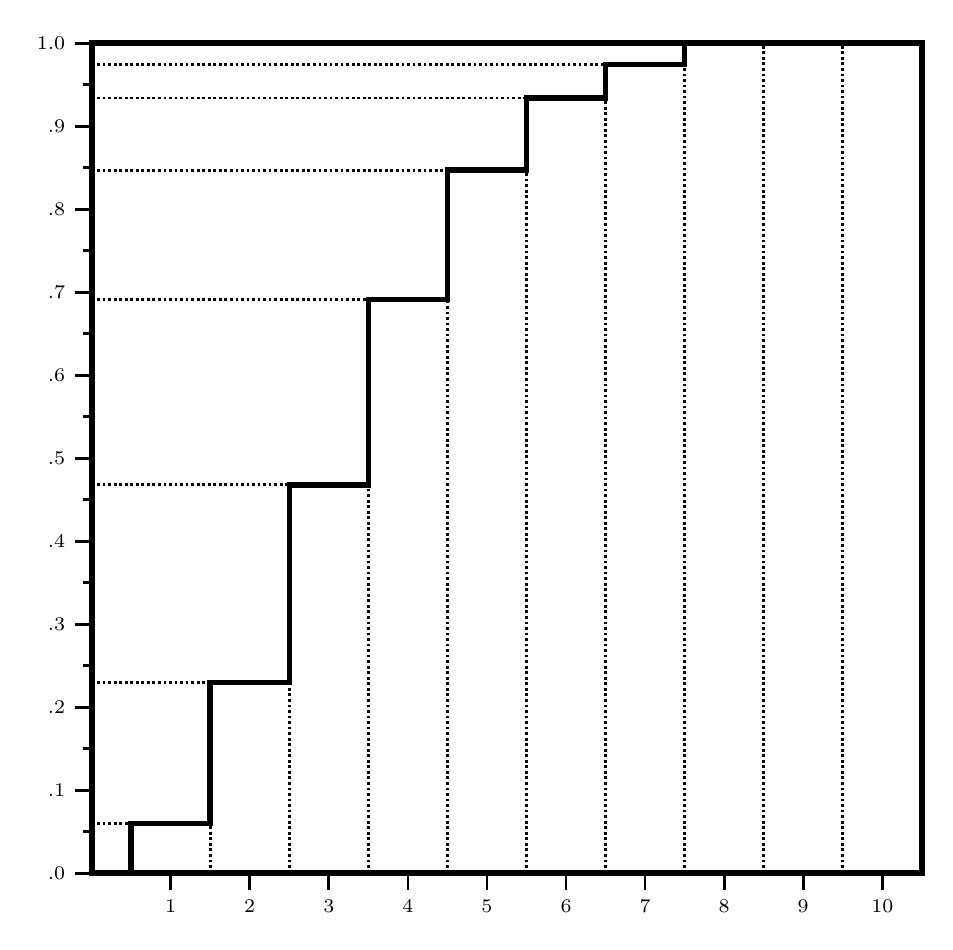
\begin{tikzpicture}
      \begin{axis}[
        width=1\textwidth,
        height=1\textwidth,
        ymin=0,
        ymax=1.0,
        xmin=0.5,
        xmax=11.0,
        ytick={0.0,0.1,0.2,0.3,0.4,0.5,0.6,0.7,0.8,0.9,1.0},
        yticklabels={\axisfont .0,\axisfont .1,\axisfont .2,\axisfont .3,\axisfont .4,\axisfont .5,\axisfont .6,\axisfont .7,\axisfont .8,\axisfont .9,\axisfont 1.0},
        xtick={1.5,2.5,3.5,4.5,5.5,6.5,7.5,8.5,9.5,10.5},
        xticklabels={\axisfont 1,\axisfont 2,\axisfont 3,\axisfont 4,\axisfont 5,\axisfont 6,\axisfont 7,\axisfont 8,\axisfont 9,\axisfont 10},
        axis lines=box,
        axis line style={line width=2.2pt},
        tick style={black,line width=1pt},
        major tick length=6pt,
        minor tick length=3pt,
        minor y tick num=1,
        tick align=outside,
        xtick pos=left,
        ytick pos=left,
        tick label style={font=\axisfont\scriptsize,/pgf/number format/assume math mode=false},
        xticklabel style={font=\axisfont\scriptsize,/pgf/number format/assume math mode=false},
        yticklabel style={font=\axisfont\scriptsize,/pgf/number format/assume math mode=false},
        enlargelimits=false,
        xmajorgrids=false,
        ymajorgrids=false,
        grid style={dotted, line width=0.6pt},
      ]
        % Figure 1.2 box: short horizontal dotted connectors from y-axis.
        \addplot[densely dotted, line width=1pt, forget plot] coordinates {(0.5,0.060) (1.0,0.060)};
        \addplot[densely dotted, line width=1pt, forget plot] coordinates {(0.5,0.230) (2.0,0.230)};
        \addplot[densely dotted, line width=1pt, forget plot] coordinates {(0.5,0.468) (3.0,0.468)};
        \addplot[densely dotted, line width=1pt, forget plot] coordinates {(0.5,0.691) (4.0,0.691)};
        \addplot[densely dotted, line width=1pt, forget plot] coordinates {(0.5,0.847) (5.0,0.847)};
        \addplot[densely dotted, line width=1pt, forget plot] coordinates {(0.5,0.934) (6.0,0.934)};
        \addplot[densely dotted, line width=1pt, forget plot] coordinates {(0.5,0.974) (7.0,0.974)};
        % Figure 1.2 box: step function (cumulative).
        \addplot[const plot,line width=2pt]
          coordinates {
            (0,0)
            (1,0.060)
            (2,0.230)
            (3,0.468)
            (4,0.691)
            (5,0.847)
            (6,0.934)
            (7,0.974)
            (8,1.000)
            (9,1.000)
            (10,1.000)
          };
        % Figure 1.2 box: vertical dotted guides at each integer.
        \addplot[densely dotted,line width=1pt] coordinates {(1,0) (1,0.060)};
        \addplot[densely dotted,line width=1pt] coordinates {(2,0) (2,0.060)};
        \addplot[densely dotted,line width=1pt] coordinates {(3,0) (3,0.230)};
        \addplot[densely dotted,line width=1pt] coordinates {(4,0) (4,0.468)};
        \addplot[densely dotted,line width=1pt] coordinates {(5,0) (5,0.691)};
        \addplot[densely dotted,line width=1pt] coordinates {(6,0) (6,0.847)};
        \addplot[densely dotted,line width=1pt] coordinates {(7,0) (7,0.934)};
        \addplot[densely dotted,line width=1pt] coordinates {(8,0) (8,1.000)};
        \addplot[densely dotted,line width=1pt] coordinates {(9,0) (9,1.000)};
        \addplot[densely dotted,line width=1pt] coordinates {(10,0) (10,1.000)};
      \end{axis}
    \end{tikzpicture}
  \end{minipage}
  \caption{Sampling the File Length Distribution}
  \label{fig:sample-file-length}
\end{figure}

A C function flength() to generate a random file length might be written as
follows. (OCR needs verification.)

\begin{verbatim}
flength ()
{
static double p[10]=
.060, .230, .468, .691, .847, .934, .974, .990, .997, 1.0;
int i = 0;
double r;
r = ranf ();
while (r > p[i]) i++;
return (i+1);
}
\end{verbatim}

There are several points about this process worth noting. First, in this
example, we can directly compute the sample value from the index to array p[]
(by adding 1). Sometimes we can do this, and sometimes we'll have to define an
array of sample values and use the index to obtain a value from the array.
Second, suppose at some place in our model we need to randomly select 1 of n
alternatives, and each alternative has a different probability associated with
it. The random selection function would look very much like the function above,
except it would return alternative numbers rather than file lengths (but if
alternatives are equiprobable, we'd probably just use an expression such as
"1+n*ranf()" to pick one).

A similar approach can be used to generate sample values from continuous
distributions. For example, suppose measurements of disk seek times give the
proportions p(ti-1,ti) of seek times falling in intervals ti-1, ti. To implement
our sampling function, we define two arrays, one containing the interval
endpoints t0, t1, t2, ... , the other containing the cumulative proportions 0,
P[t<t1], P[t<t2], ... . To generate a sample value, we generate a random number
r and use it to find the entry in the array for which P[t<ti-1] < r < P[t<ti].
The sample seek time is determined by interpolation between the corresponding
entries in the seek time interval endpoint array. The sample-generating
statements might look like this (OCR needs verification):

\begin{verbatim}
r = ranf ();
while (r > p[i]) i++;
t = t[i-1] + (t[i]-t[i-1]) * (r - p[i-1]) / (p[i] - p[i-1]);
\end{verbatim}

There are several things we can do (in addition to coding changes) to make
sample generation more efficient. If there are more than a few entries, we can
use a binary, rather than a linear, search of p[]. The intervals used to divide
the distribution don't have to be the same width; we can use short intervals
where the distribution changes shape rapidly and long intervals where the rate
of change is slow to optimize the number of entries.

In both examples, we tabulated the cumulative distribution function p = F(x),
generated a random value of p, and used the tabulation to obtain the
corresponding value of x; in effect, we generated values of the inverse
function \ensuremath{x = F^{-1}(p)}. In some cases, it is possible to determine directly the
inverse of the distribution function of a theoretical distribution. For
example, suppose inter-arrival times are exponentially distributed with mean T;
the probability that an arrival time x is equal to or less than t is given by

\begin{align}
\Pr[x<t] &= 1 - e^{-t/T} \tag{1.1}\label{eq:exp-cdf}\\
t &= -T \ln(1-r) \tag{1.2}\\
t &= -T \ln r \tag{1.3}
\end{align}

where ln(x) denotes the natural logarithm of x. Since r is a random variate
uniformly distributed in [0,1], 1-r is identically distributed; therefore, we
can rewrite (1.2) as (1.3). We can use (1.3) to write a C function to generate
sample values from the exponential distribution. The following function is one
of the smpl random variate generation functions.

\begin{verbatim}
double expntl (t)
double t;
{
  double ranf();
  return (-t*log(ranf()));
}
\end{verbatim}

Unfortunately, direct inversion of the distribution function is possible only
for a few distributions; other techniques for generating variates frequently
are needed. For most of our simulation work, we'll manage with the smpl
sampling functions supplemented by those presented in our simulation texts.
Nevertheless, familiarity with random variate generation techniques is useful;
among other things, it provides ideas for incorporating analytic results in our
simulation models. Of course, if pressed, we can tabulate values of the
distribution function for any discrete or continuous distribution, and generate
samples as we did in our earlier examples.

There are a few things to keep in mind when sampling theoretical distributions.
First, do the values returned by your random number generator include 0? If so,
you will have to be sure that your sampling functions don't attempt to take the
logarithm of a zero value. Theoretical distributions may have tails extending
to infinity on one or both sides, and samples may need to be clipped. Most
variables in computer system simulations don't have negative values: when
sampling from the normal distribution, inspect samples and discard negative
values. Generators for distributions such as the exponential distribution can
return very large values; you may want to truncate the sample distribution to
reflect the maximum value realizable in the actual system. The mean value of
samples from (for example) a truncated exponential distribution may differ from
the exponential distribution's mean unless the latter is adjusted. Section 6.8
discusses computation of an adjusted mean for a truncated exponential
distribution.

\paragraph{Correlation.}
There are two kinds of correlation that may need be represented in a model. One
is autocorrelation, where successive values from a distribution are not
independent but reflect some underlying relationship. This is a difficult
subject in terms of both workload characterization and model representation.
Fishman [1978] describes two ways of generating autocorrelated sequences.

The second kind of correlation is that between jointly-distributed variables:
variables from different distributions representing different aspects of work.
For example we would expect compiler execution times and compiler input file
lengths to be correlated, in which case a functional relationship could be
obtained via regression analysis of measurement data. To generate attributes
of a particular compilation in a simulation model, we could generate a sample
input file length and use its value to compute a sample compilation time.
Modeling such relationships mostly involves common-sense tradeoffs between
model accuracy and complexity. Developers of synthetic workloads face similar
problems and have developed sampling approaches: see, for example, Hughes
[1984], and Sreenivasan and Kleinman [1974].

\section{A Simple Queueing Simulation}
\label{sec:simple-queueing-sim}

This section presents a simulation model of a simple queueing system written in
C without the use of smpl. We'll review some of the performance measures of
interest in queueing system analysis and discuss basic simulation operations.
First, let's look at how queueing systems are described.

Queueing notation. A standard notation (called Kendall notation after its
originator) is used to describe queueing systems with a single queue and one or
more parallel servers. This notation is commonly used in the literature, so
it's useful to be familiar with it. Using this notation, a queueing system is
described by a descriptor of the form A/S/c/k/m, where A represents the
inter-arrival time distribution, S represents the service time distribution, c
is the number of servers, k is the maximum number of customers allowed in the
system, and m is the number of customers available at the source.\footnote{Use
of the term ``customer'' to describe a system's work-bearing entities and
``server'' to describe its work-performing entities is traditional. Also,
``queueing system'' frequently is shortened to ``queue''.} Among the symbols
commonly used to describe distributions are:

\begin{verbatim}
D   constant inter-arrival or service time
M   exponential distribution
Ek  k-Erlang distribution
Hk  k-stage hyperexponential distribution
G   general (arbitrary) distribution
\end{verbatim}

When the customer population is assumed to be infinite, m usually is omitted;
similarly, when the system capacity is assumed to be infinite, k is omitted.
The queueing discipline may be appended to the descriptor; if not, it can be
assumed to be first-in, first-out. Using this notation, a queueing system with
exponential inter-arrival times, constant service times, and a single server is
described as an M/D/1 queue; a system with exponential inter-arrival times,
general service times, 2 servers, and a queue capacity of k customers is
described as an M/G/2/k queue.

The queueing system model. The system to be simulated is the single server
queueing system shown in Figure 1.3. Work for the system comes from an
infinite population of customers; the inter-arrival times of customers at the
system are exponentially distributed with mean Ta. On arrival, a customer
begins service if the server is free or joins the queue if the server is busy.
The queue capacity is unlimited, and the queueing discipline is first-in,
first-out; whenever one customer completes service, the next customer to begin
service is the one at the head of the queue. Service times are exponentially
distributed with mean Ts. (This, then, is an M/M/1 queue.)

\begin{figure}[htbp]
  \centering
  \fbox{\parbox{0.8\textwidth}{TODO: Figure 1.3. A Single Server Queueing System}}
  \caption{A Single Server Queueing System}
\end{figure}

The C program of Figure 1.4 is a simulation model of this system, and is about
as simple as we can get. It uses the expntl() function discussed in the last
section to generate inter-arrival and service times. The mean inter-arrival
time Ta is 200 time units, the mean service time Ts is 100 time units, and the
period of time to be simulated, te, is 200000 time units (so we would expect to
simulate approximately 1000 arrivals). time represents simulated time, and n
is the number of customers in the system at any point in time. There are two
events: event 1 represents arrivals and event 2 represents service completions.
Associated with events 1 and 2 are the event occurrence times t1 and t2; these
are the times at which the next instance of the event will occur.

The model advances through time in variable intervals, rather than constant
"ticks". At any instant, t1 is the time of the next arrival and t2 is the time
of the next completion; to determine which event occurs next, these times are
compared. If t1<t2, then the next event is an arrival. time is advanced to the
arrival time, the count of the number of customers in the system is incremented,
and the time at which the next arrival is to occur is computed. If the system
was empty when this customer arrived, the time at which its service will
complete is computed. If t1>t2, then the next event is a service completion:
time is advanced to the completion time and the number of customers in the
system is decremented. If there are still customers in the system after this
completion, then the time of the next service completion is computed. (This
implicitly represents dequeueing of the customer at the head of the queue and
the start of its service.) If the current completion empties the system, t2 is
set to te to insure that the next event to occur will be an arrival; note that
this also was done during initialization to insure that the first event would
be an arrival.

\begin{figure}[htbp]
  \centering
  \begin{minipage}{0.9\textwidth}
    \begin{verbatim}
main ()
{
double Ta=200.0,Ts=100.0,te=200000.0,t1,t2,time;
double expntl();
int n;
n=0; t1=0.0; t2=te; time=0.0;
while (time<te)
{
if (t1<t2)
{ /* event 1: arrival */
time=t1; n++; t1=time+expntl(Ta);
if (n==1) t2=time+expntl(Ts);
}
else
{ /* event 2: completion */
time=t2; n--;
if (n>0) t2=time+expntl(Ts); else t2=te;
}
}
}
    \end{verbatim}
  \end{minipage}
  \caption{Queueing System Simulation Model}
\end{figure}

Figure 1.5 graphically illustrates the behavior of the simulated system.
Suppose we observe the system for a period of 600 time units, during which
customers arrive at intervals (i.e., inter-arrival times) of 20, 30, 25, 65, 80,
and 80 time units. The service times of these customers are, respectively, 80,
150, 90, 60, 80, and 90 time units. Figure 1.5(a) shows the sequence of
arrivals, waiting times, and service times in the period; Figure 1.5(b) shows
the corresponding changes in the number of customers in the system. If we
manually step through the simulation program using the above inter-arrival and
service times, we can see how the model generates this behavior.

\begin{figure}[htbp]
  \centering
  \fbox{\parbox{0.8\textwidth}{TODO: Figure 1.5. Queueing System Behavior}}
  \caption{Queueing System Behavior}
\end{figure}

\section{Performance Measures}
\label{sec:performance-measures}

While the program of Figure 1.4 may successfully model the behavior of an M/M/1
queueing system, it isn't of much use until we add instrumentation to collect
the performance measures of interest to us. We can collect just about
anything; mostly we'll be interested in mean values, but on occasion we may
want distributions as well. We'll begin this section with a look at certain
fundamental mean value performance measures and their relationships. Because
these relationships apply widely and hold under very general conditions, some
have come to be called laws.

Suppose we observe the system for a period of time T and measure the number of
arrivals, A, and the number of completions, C. We then can compute the arrival
rate and the throughput rate:

\begin{align}
A &= A/T \tag{1.4}\\
X &= C/T \tag{1.5}
\end{align}

In measuring a real or simulated system, there may be customers in the system
queued for or receiving service both at the start and at the end of the
observation period.
However, if the period is sufficiently long, the number of arrivals observed
should be approximately equal to the number of completions (C = A), in which
case we can assume A = X. This assumption is called the flow balance
assumption: the flow of work out of the system is balanced by the flow of work
into it. When we make this assumption, we only need to count arrivals or
completions, whichever is easier, not both.

Suppose we also measure the mean server busy time, B. Now we can compute the
server utilization and the mean service time per customer:

\begin{align}
U &= B/T \tag{1.6}\\
T_s &= B/C \tag{1.7}
\end{align}

Utilization Law. Through simple algebra, we can combine (1.5), (1.6), and (1.7)
to obtain the Utilization Law:

\begin{align}
U &= X T_s \tag{1.8}\\
U &= A T_s \tag{1.9}
\end{align}

In words, the utilization of a server is the product of its
throughput rate and the average service time per customer.

Little's Law. Let L be the average number of customers in the system during
the observation period, and let W be the average time these customers spend in
the system. Define \ensuremath{w_i} as the time spent in the system by the ith customer:
then \ensuremath{W = \sum w_i / C}. Look back at Figure 1.5(b) for a moment; this is a graph
of the number of customers in the system versus time. The average number of
customers in the system is the average height of the graph; this is equal to
the area under the graph divided by the length of the observation period. Each
customer, while in the system, contributes one unit of height to the graph, and
so contributes 1 x wi to the area under the graph. The total area is the sum
of the contributions of the C customers completing service during the
observation period, which is equal to W C. The average number in the system is
this area divided by the observation time: \ensuremath{L = W C / T}. Since, from (1.5),
\ensuremath{C/T = X}, we can write

\begin{align}
L &= X W \tag{1.10}\\
L &= A W \tag{1.11}
\end{align}

In words, the average number of customers in the system is the product of the
system's throughput rate and the average time a customer spends in the system.

The preceding paragraph gave an informal derivation of Little's Law, named for
J. D. C. Little, who presented the first formal proof [Little 1961]. This law
is one of the most important results in queueing theory (the mnemonic of "law"
for L = AW makes it easy to remember). It doesn't depend on the form of the
inter-arrival or service time distributions or on the queue discipline. Little's
Law can be applied at various levels of a system and in various ways at a given
level. For example, let Lq be the average number of customers queued in the
system (not receiving service), and let \ensuremath{W_q} be the mean queueing time. We can
use the same approach as before to show that

\begin{equation}
L_q = A W_q \tag{1.12}
\end{equation}

Note that \ensuremath{L = L_q + U} and \ensuremath{W = W_q + T_s}. We can consider the Utilization Law to be another
application of Little's Law by viewing U as the average number of customers
receiving service.\footnote{In queueing theory literature, the time a customer
spends in the system -- including service time -- usually is called "waiting
time". (This isn't intuitive to the designer, who separates working time and
waiting time.) Similarly, the term "queue length" is used to describe the
number of customers in the system, including those in service. (Always read the
definition of terms carefully.) We'll call the time a customer spends in the
system its system residence time or its response time, and the time it spends
in the queue (not receiving service) its queueing time.}

Response Time Law. This law commonly is stated in the context of a timesharing
system. Let N be the number of terminals in the system, let Z and R be,
respectively the mean think time and mean response time at a terminal, and let
X be the system throughput. Then

\begin{equation}
R = (N/X) - Z \tag{1.13}
\end{equation}

An example of the use
of this law in a different context is given in Section 5.3.

Let's apply some of these relationships to the queueing system whose behavior
is represented in Figure 1.5. There are C = 6 completions in the observation
period of T = 600 time units. (Arrival, service start, and service completion
times can be obtained by reference to the event times along the time axis of
Figure 1.5(b)).

\begin{align*}
\text{throughput:} &\quad X = 6/600 = 0.01\\
\text{total busy time:} &\quad B = (100-20)+(250-100)+\cdots+(570-480) = 550\\
\text{mean service time:} &\quad T_s = 550/6 = 91.7\\
\text{utilization:} &\quad U = 550/600 = 0.917 \;\text{or}\; 0.01 \times 91.7 = 0.917\\
\text{residence time sum:} &\quad \sum w_i = (100-20)+(250-50)+\cdots+(570-300) = 1335\\
\text{mean residence time:} &\quad W = 1335/6 = 222.5\\
\text{mean queueing time:} &\quad W_q = 222.5 - 91.7 = 130.8\\
\text{mean number in system:} &\quad L = 1335/600 = 2.225\\
\text{mean number in queue:} &\quad L_q = 2.225 - 0.917 = 1.308
\end{align*}

Little's Law, the Utilization Law, and other important relationships can be
derived under relatively pragmatic assumptions by taking an operational view of
system behavior. This view was pioneered by J. P. Buzen [Buzen 1976] and by
P. J. Denning. Careful reading of their tutorial paper [Denning and Buzen 1978]
and of the discussion by Lazowska et al [1984] is recommended strongly.

\section{Instrumenting the Model}
\label{sec:instrumenting-the-model}

In a simulation model, the observation period T often corresponds to the
simulation period, although it will be less when the first part of a simulation
run is discarded to eliminate "warm-up" effects (discussed in Chapter 4). For
each server in our model, we need to maintain a count C of the number of
service completions and a sum B of the server busy times. When the simulation
completes, the throughput, utilization, and mean service time of each server
can be computed from T, C, and B.

There are two ways we can instrument the model to get the mean number in queue
and service L, and the mean residence time W. One way is to accumulate the
residence times of customers as they complete service; when the simulation
completes, this sum is divided by C to obtain the mean residence time, and then
Little's Law is used to compute L. This has one drawback; it requires that each
customer be timestamped as it arrives at each server, and this can add unwanted
complexity to the model (our M/M/1 queue doesn't even distinguish customers
from one another).

Another approach is to compute L directly. Once again, look back at Figure
1.5(b). The average number of customers in this system is the area under this
graph divided by the observation period. Earlier, we computed this area by
summing the residence times of each customer. However, this area also is the
sum of the areas of a set of rectangles; the height of each rectangle is the
number of customers in the system, and the base is the time interval between
changes in this number. This suggests an algorithm for computing L. Define
variables s and tn, and assume n represents the number of customers in the
system. At the start of the observation period, set s to 0 and set tn to the
current simulation time, time. Each time a customer arrives in the system,
perform:

\begin{verbatim}
s += n * (time - tn); n++; tn = time;
\end{verbatim}

and each time a customer completes service, perform:

\begin{verbatim}
s += n * (time - tn); n--; tn = time;
\end{verbatim}

to compute and sum the areas of the individual rectangles. When the simulation
completes, the average number in the system is computed by dividing s by the
observation period length, and the average residence time then computed using
Little's Law.

This approach is used in the instrumented version of the M/M/1 queue simulation
model shown in Figure 1.6. Most of the variables added in this version are
named in accordance with the measures they represent: e.g., C is used to count
service completions. Variables B and tb are used to accumulate total server
busy time. A server busy period begins when an arriving customer finds the
system empty and immediately begins service; the event 1 section computes its
service completion time and sets tb to the current simulation time. A server
busy period ends when a customer completes service and there is no other
customer in the system; the event 2 section computes the length of the busy
period just ended and adds it to B.

\begin{figure}[htbp]
  \centering
  \begin{minipage}{0.9\textwidth}
    \begin{verbatim}
main ()
{
double Ta=200.0,Ts=100.0,te=200000.0,t1,t2,time;
double B,C,L,s,tb,tn,U,W,X,expntl();
int n;
n=0; t1=0.0; t2=te; time=0.0;
B=s=0.0; C=0; tn=time;
while (time<te)
{
if (t1<t2)
{ /* event 1: arrival */
time=t1; s+=n*(time-tn); n++; tn=time;
t1=time+expntl(Ta);
if (n==1) {tb=time; t2=time+expntl(Ts);}
}
else
{ /* event 2: completion */
time=t2; s+=n*(time-tn); n--; tn=time; C++;
if (n>0) t2=time+expntl(Ts);
else {t2=te; B+=time-tb;}
}
}
X=C/time; printf ("throughput = %f\n", X);
U=B/time; printf ("utilization = %f\n", U);
L=s/time; printf ("mean no. in system = %f\n", L);
W=L/X; printf ("mean residence time = %f\n", W);
}
    \end{verbatim}
  \end{minipage}
  \caption{Instrumented Queueing System Simulation Model}
\end{figure}

\section{Basic Simulation Operations}
\label{sec:basic-simulation-operations}

The model of Figure 1.6 can be extended in certain ways without difficulty. We
can change inter-arrival and service time distributions, limit system capacity,
and so on. However, if we try to extend this approach to systems with several
servers, next event selection by direct comparison of event occurrence times
quickly gets unwieldy; an event list scheduling mechanism provides a simpler
and yet more general approach.

The event list scheduling mechanism comprises a procedure for scheduling
events, a procedure for selecting -- "causing" -- the next event, a variable
representing the current value of simulated time, and the event list data
structure itself. When an event, such as the arrival of the next customer, is
to be scheduled, the schedule procedure is called to create and add an entry to
the event list. This entry includes the event occurrence time, the identity of
the event to occur, and often the identity of the associated customer. The
event list is ordered in ascending values of event occurrence times; the new
entry is linked into the list at a position determined by its event occurrence
time. Whenever the simulation program completes all processing at a given
instant in simulation time, it calls the cause procedure to determine which
event is to occur next. cause removes the entry at the head of the event list,
advances simulation time to the event occurrence time contained in the entry,
and returns the identity of the event (and of the customer, if included). The
simulation program then initiates execution of that event.

Since the event list mechanism is a general one, we implement it to be reusable
and place it in a simulation function library -- which probably got its start
with our random variate generation functions.

The system being simulated frequently comprises a number of facilities, such
as disks, channels, and processors. While these differ physically, their model
representations have much in common. Each can be set busy or non-busy, each can
have requests queued for it, and each requires similar performance measures.
Consequently, we are led to develop a generic model of facilities, and provide
functions for facility creation and manipulation; these also are added to the
library. The need for report generation, debugging aids, and similar
capabilities results in further additions, and we eventually end up with a
simulation library, or subsystem, something like smpl. Although we may not have
the power of some of the current simulation languages, we can do our modeling
in a language of our choice, and we can tailor our simulation functions to suit
our needs.

Lists in general and event lists in particular came into common use in the
early 1960s. Event selection by direct comparison of event times was described
in one of the first books on discrete-event simulation, "The Art of
Simulation", by K. D. Tocher [1963].

\section{A smpl Queueing Simulation}
\label{sec:smpl-queueing-simulation}

We'll conclude this chapter and preview the next with a look at a smpl
simulation model version of the M/M/1 queue; the simulation program is shown in
Figure 1.7. The names of smpl functions are underlined for emphasis. Floating
point variables are declared as real, which the user can define as either float
or double (via a typedef in smpl.h), based on space and possibly time
considerations.

There are three initialization steps: smpl() is called to initialize the
simulation subsystem and name the model, facility() to create and name a
facility representing the queueing system's server, and schedule() to schedule
the first customer arrival. (This model doesn't distinguish customers; the
value of customer remains unchanged during model execution.) The schedule()
function adds the specified inter-event time -- 0, in this case -- to the
current simulation time (which is initially 0) to obtain the event occurrence
time, and creates an event list entry containing the event occurrence time, the
event number, and the customer number. The period of the simulation is
controlled by the while statement; the time() function returns the current
simulation time.

The cause() function removes the entry at the head of the event list, advances
simulation time to the event occurrence time of that entry, records the event
number as the current event, and returns the event and customer numbers. The
program uses the event number to select the next event to be executed.

This model is divided into three events (our earlier model had two events).
Event 1 represents a customer arrival; it schedules the server request of the
arriving customer for immediate occurrence, and schedules the next arrival.
Event 2 is a server request. If the server is free, the request() function
reserves it for the requestor, returning 0 to indicate that the request was
successful, and the customer's service completion is scheduled. If the server
is busy, request() queues the request and returns 1 to indicate its action. The
queue entry includes the customer and the current event.

Event 3 represents a service completion: release() is called to release the
server. If a request has been queued, release() dequeues it, creates an event
list entry for it, and puts this entry at the head of the event list. This
entry has an event occurrence time equal to the current time, and its event
number and customer are those recorded when the request was queued. The next
call to cause(), then, will result in the execution of event 2 for the dequeued
request. This implicit invocation of an event is the reason for the separation
of the arrival and server request events in this model.

\begin{figure}[htbp]
  \centering
  \begin{minipage}{0.9\textwidth}
    \begin{verbatim}
#include <smpl.h>
main ()
{
real Ta=200.0,Ts=100.0,te=200000.0;
int customer=1, event, server;
smpl (1, "M/M/1 Queue");
server=facility("server",1);
schedule (1,0.0, customer);
while (time ()<te)
{
cause (&event, &customer);
switch (event)
{
case 1: /* arrival */
schedule (2,0.0, customer);
schedule (1,expntl(Ta), customer);
break;
case 2: /* request server */
if (request (server, customer, 0)==0)
schedule (3,expntl(Ts), customer);
break;
case 3: /* completion */
release (server, customer);
break;
}
}
report ();
}
    \end{verbatim}
  \end{minipage}
  \caption{smpl Queueing System Simulation Model}
\end{figure}

When the simulation completes, report() is called to generate the simulation
report. The data given in this report includes the period of the simulation,
server utilization, server mean busy period, mean queue length, number of
requests completed, and the number of times requests were queued. The model
parameters specified in Figure 1.7 result in the simulation of 1025 customer
service completions; the reported utilization is 0.5301, the mean busy period
is 103.482, and the mean queue length is 0.659.

\section{Problems}
\label{sec:intro-problems}

Some of these problems require a random number generator. You can use the one
provided in your C library, or you can use the smpl ranf() function described
in Chapter 8; code for this function is given in the Appendix.

\begin{enumerate}
  \item In modeling program behavior, the number of instructions executed from
    consecutive memory locations, beginning with the target of a taken branch
    instruction and ending with (and including) a taken branch instruction,
    sometimes is called the headway between branches. Measurement data collected
    during the execution of a particular system workload provided the following
    distribution of inter-branch headways; \ensuremath{p_h} is the proportion of
    headways of length h.

    \begin{verbatim}
    h   ph     h   ph     h   ph     h   ph
    1  .0659   9  .0261  17 .0108  25 .0020
    2  .0750  10  .0432  18 .0115  26 .0023
    3  .1106  11  .0169  19 .0069  27 .0045
    4  .1054  12  .0111  20 .0144  28 .0018
    5  .0978  13  .0116  21 .0113  29 .0015
    6  .0758  14  .0179  22 .0025  30 .0018
    7  .0660  15 .0095   23 .0044  31 .0005
    8  .0502  16 .0108  24 .0052  32 .0074
    \end{verbatim}

    Headways of length 1 indicate that the target of a taken branch is itself a
    taken branch; this results from some procedure call protocols and from
    transfers via branch vector tables. The proportion of headways greater than
    127 can be assumed to be 0. The mean headway H is 6.957 instructions (the
    reciprocal of H is the proportion of instructions which are taken branches).
    Plot a histogram of the headway distribution, and write a function to
    generate random variates from this distribution. (In deciding how to
    generate headways in the range 32-127, consider the shape of the
    distribution and the difference between H and \ensuremath{\sum h p_h, 1<h<31}.) Generate
    5000 sample headway values and compare their distribution with that of the
    measured headways.

  \item The histogram of the headway distribution suggests that it can be
    modeled as a mixed distribution, composed of a constant distribution for
    headways of 1 and a geometric distribution for headways greater than 1.
    Assuming this form, the following model can be derived:

    \begin{equation}
      \Pr[h=i] =
      \begin{cases}
        p_1, & i = 1 \\
        (1-p_1)p(1-p)^{i-2}, & i > 1
      \end{cases}
      \tag{1.14}
    \end{equation}

    where p1 is the proportion of headways equal to 1 (0.0659), and
    \ensuremath{p = (1-p_1)/(H-1)}.\footnote{There are other ways to fit the
    parameters of this model to the measurement data; the choice depends on
    what characteristics of the data it is desired to preserve.} The geometric
    distribution parameter p is determined from the contribution of the
    geometric part of the mixed distribution to the mean:

    \begin{equation*}
      (1-p_1) \sum_{h=2}^{\infty} h p (1-p)^{h-2} = H - p_1
    \end{equation*}

    (a) Visually check how well this model matches the headway distribution by
    overlaying a plot of (1.14) on the headway distribution histogram. To
    compare the tails of the measured and modeled distributions, compute and
    plot the log survivor function \ensuremath{\ln(\Pr[h>i])} versus i for each distribution.
    (b) Determine, quantitatively, how well the distribution defined by (1.14)
    matches the measurement data. Refer to a statistics text for methods.
    (c) For the geometric distribution \ensuremath{p_k = p(1-p)^k, 0<k<\infty, 0<p<1}, a sample
    variate k can be generated from (see, for example, Law and Kelton [1982]):

    \begin{equation}
      k = \lfloor \ln r / \ln(1-p) \rfloor \tag{1.15}
    \end{equation}

    where \ensuremath{\lfloor x \rfloor} denotes the floor function of x -- the largest integer equal to
    or less than x -- and r is a uniform random variate. Using (1.15), write a
    function to generate sample headway values from the distribution defined by
    (1.14). Generate 5000 sample headway values and compare their distribution
    with that of the measured headways. (Save this function for use in the
    pipeline analysis project of Chapter 5.)

  \item If all we know about a variable X is that its values fall within a
    range [a,b], we'll probably use a uniform distribution to generate values
    of X. Given an estimate of the most likely value (mode) of X, we can use a
    triangular distribution to model X. The triangular distribution is defined
    by its range [a,b] and mode c; its mean is (a+b+c)/3. Figure 1.8 shows a
    sketch of the density function of this distribution and gives its
    distribution function \ensuremath{F(x) = \Pr[X<x]}.

    \begin{figure}[htbp]
      \centering
      \fbox{\parbox{0.8\textwidth}{TODO: Figure 1.8. Triangular Distribution}}
      \caption{Triangular Distribution}
    \end{figure}

    Sketch the distribution function for the triangular distribution. What is
    the value of F(x) at x = c? Let \ensuremath{p = F(X)}, and determine the inverse of the
    distribution function \ensuremath{F^{-1}(p)}. Use this inverse function to write a
    random variate generator for the triangular distribution. Check the
    generator by picking values for a, b, and c, generating a large number of
    sample values, and comparing the sample and theoretical distributions.
    (Save the function for use in the timesharing model of problem 3, Chapter
    2.)

  \item A small timesharing system (Figure 1.9) has 16 user terminals connected
    to a minicomputer system with two disks. A user "thinks" for a time z and,
    at the end of that time, sends a request to the computer system and waits
    for the system to respond. When the response is received, the user thinks
    again and then initiates another request.

    \begin{figure}[htbp]
      \centering
      \fbox{\parbox{0.8\textwidth}{TODO: Figure 1.9. Timesharing System}}
      \caption{Timesharing System}
    \end{figure}

    Operating system instrumentation shows that the system processes 2 terminal
    requests per second with an average response time per request of 3 seconds;
    the CPU utilization is 95 percent.

    (a) What is the mean user think time?
    (b) On average, how many users are thinking and how many are waiting for
    requests to be processed by the computer system?
    (c) Each terminal request generates an average of 12 CPU-disk operations.
    What is the mean CPU execution time for each such operation?
    (d) Measurements show that the average CPU queue length is 4.25. Assuming
    that requests either are competing for CPU service or for disk service
    (i.e., no memory queueing), what is the mean disk residence time per disk
    operation?
    (e) How would you instrument the system to obtain data to estimate the mean
    disk operation queueing time?

  \item Our modeling work usually will focus on queueing systems of various
    kinds. However, you'll sometimes find it handy to use simulation to analyze
    other types of problems and as a check on analytic solutions. This and the
    following two problems provide simple examples of this use of simulation.
    The graph of Figure 1.10 represents a computer program. Diamonds represent
    branch instructions; each branch path is labeled with the probability of
    its being taken on any given execution of the branch instruction. This
    probability is independent of the path taken on previous branches.
    Rectangles represent non-branch instructions. Write a simulation model of
    this program to determine the average number of instructions executed;
    simulate 1000 program executions.

    \begin{figure}[htbp]
      \centering
      \fbox{\parbox{0.8\textwidth}{TODO: Figure 1.10. Program Graph}}
      \caption{Program Graph}
    \end{figure}

  \item A certain allocation mechanism allocates elements from two lists.
    Whenever an allocation request is received, one of the two lists is
    selected at random and an element allocated from that list. Write a
    simulation program to determine the average number of elements remaining in
    one list at the instant the other list is empty, assuming that each list
    initially contains 16 elements. Simulate 1000 list emptyings.

  \item A table comprising a set of records organized in increasing order of
    key field values, K1 < K2 < ... < KN, is searched for a key value A using a
    binary search algorithm (see, e.g., Knuth [1973]). This algorithm first
    compares A to the value in the middle of the table. The result of this
    comparison is used to determine which half of the table to examine next,
    and A is compared with the middle key of the selected half. This process is
    repeated until the desired record is found (or until it has been determined
    that the record is not in the table). The number of comparisons required
    for a successful search is in the range [1,m], where \ensuremath{2^{M}-1 < N < 2^{M}}; the
    average is about \ensuremath{\ln N - 1}. Write a simulation program to determine the
    distribution of the number of comparisons required for a successful search
    as well as the mean number. Assume that N = 63 and that A equiprobably is
    one of the key values K1, K2, ..., KN (so that A always is found in the
    table). Simulate 1000 searches.
\end{enumerate}

% OCR draft from PDF pages 51-82. Needs cleanup and verification.
\chapter{smpl}
\label{chap:smpl}

\section{The smpl View of Systems}
\label{sec:smpl-view-of-systems}

At the start of the previous chapter, we discussed the dynamic and static
composition of systems in general terms. In this section, we'll discuss a more
specific view appropriate to the nature of our tools. In the smpl view of
systems, there are three kinds of entities: facilities, tokens, and events.

Facilities. In static form, a system comprises a collection of interconnected
facilities. A facility typically represents some work-performing resource of
the system being modeled, such as the CPU in a computer system or the bus in a
local area network model. Facilities also may represent resources other than
hardware, such as a software lock in an operating system. smpl provides
functions to define facilities, reserve, release, and preempt them, and
interrogate their status. The interconnection of facilities is not explicit,
but rather is determined by the model's routing of tokens between facilities.

Tokens. Tokens represent the active entities of the system; the dynamic
behavior of the system is modeled by the movement of tokens through a set of
facilities. A token may represent a task in a computer system model, a packet
in a communications network model, or a memory access in a memory bus
subsystem model. smpl provides two basic kinds of operations for controlling
the flow of tokens through the simulated system; a token may reserve (or
preempt) facilities, and it may schedule activities of various durations. If a
token attempts to reserve an already-busy facility, it is queued until the
facility becomes available to it. From a timing standpoint, the flow of a
token through the system can be described by its sequence of delay (queueing)
and activity times.

What a token represents is up to the modeler; as far as the smpl simulation
subsystem is concerned, a token is just an integer. The only attribute of a
token which the simulation subsystem knows about is its priority. In some
models it is not necessary to distinguish between instances of work, as in the
queueing model of Figure 1.7; in this model, the token represented
indistinguishable customers and was a simple variable whose value remained
unchanged over the course of the simulation. In other models, tokens may be
indexes to arrays whose elements contain attributes of the work, such as the
compute time, memory size, and number of I/O requests for a task in a computer
system model.

Events. A change of state of any system entity, active or passive, is an
event. Suppose a task (or process) completes a CPU execution interval and
releases the CPU. Two events have occurred: an activity of the task ended, and
the CPU changed state. The termination of one activity of the task may cause
initiation of another of the same task; release of the CPU may result in
execution of some earlier-initiated activity of some other task. In
event-oriented simulation languages such as smpl, we usually collect together
actions which take place at any one instant in time, and tend to think of this
collection as an event. This casual view isn't much of a problem in building
small models; however, in developing complex models, an amazing number of
problems can be avoided by distinguishing individual events and organizing the
model accordingly. We'll revisit this subject in Chapter 3.

smpl provides functions for scheduling events and for selecting -- ``causing''
-- events in order of their event occurrence times. From the standpoint of the
simulation subsystem, an event is identified by its number, the simulation
time at which it is to occur, and possibly the identity of a token involved
with the event. What the event represents is up to the modeler; it frequently
will correspond to several system events.

A smpl simulation program comprises an initialization routine, a control
routine, and some number of event routines. A ``routine'' may range in size
from a single statement to a large subprogram, depending on the model's
complexity. The control routine selects the number of the next event to occur
and transfers control to the appropriate event routine which, typically,
schedules one or more other events and then returns to the control routine.
When talking about simulation programs, we'll sometimes become even more
casual in our terminology, and refer to event routines simply as events.

\section{Function Descriptions}
\label{sec:smpl-function-descriptions}

The functions provided by smpl for simulation modeling, testing, and
experimentation are described in following sections. First, we'll discuss
initialization, facility, event scheduling, and random variate generation
functions, and use these to develop a queueing network simulation model.

Next, using this model as an example, we'll review smpl's debugging and report
generation functions.

smpl function descriptions begin with a two-line synopsis. The first line
shows the function and its formal parameters. When a function returns a value,
it is shown assigning a value to a dummy parameter as, for example, in
\ensuremath{n = inq(f)}. The second line of the synopsis shows the types of the
parameters. Real-valued parameters are of type real, which can be defined as
either float or double. Generally, smpl systems and models define real as
double, but space considerations sometimes might dictate its definition as
float. In either case, definition is accomplished via typedef declarations in
smpl subsystem source programs and in the smpl.h file.

smpl.h contains external declarations for smpl functions, \#include's for
stdio.h and math.h, the typedef declaration for real, and the \#define for the
pseudo-keyword then. smpl.h should be included in all smpl simulation
programs. (A listing of smpl.h appears in the Appendix.)

Function descriptions tend to be dry reading in any event, and those of the
following sections are intended to be detailed enough for your use as
reference to smpl. So, give them a quick first reading, see how the functions
are used in the queueing network simulation model, and reread the
descriptions of those functions about which you have questions. When you
start coding your first model, read through the descriptions once again. A
short tabulation of the most commonly-used smpl functions appears at the end
of this chapter.

\section{Model Initialization}
\label{sec:smpl-model-initialization}

\begin{verbatim}
smpl (m, s);
int m; char *s;

reset ();
\end{verbatim}

The smpl() function initializes the simulation subsystem for a simulation run.
m is 1 if mtr is to be activated, and 0 if it is not. When using the
implementation of smpl presented in this book, m should always be 0. mtr,
part of the SMPL simulation environment, provides an interactive interface to
model execution; some of its facilities are described in Chapter 7. While its
implementation isn't included here, an overview of its design is given in
Chapter 9, and you may want to add a similar capability in your system. The
``hooks'' between smpl and mtr -- there are only a few -- have been left in
place to keep the smpl source code given in the appendix identical to that in
the SMPL system. s is a pointer to the model's name; the name (limited to 50
characters) appears as a heading on the simulation report.

smpl() initializes and clears data structures, and sets both simulation time
and the start of the current measurement interval to zero. smpl accumulates
measurement data continuously during model execution. Normally, the
simulation interval (the period of time simulated) and the measurement
interval coincide, and the performance measures given in the simulation report
are averaged over the complete simulation run. However, executing a reset()
function clears all accumulated measurements; the time at which this function
is called becomes the start of the measurement interval, and the reported
measures represent model activity only from that time to the time at which the
report is generated. We may want to use this capability to discard data
collected while the model is ``warming up'' in order to eliminate
initialization bias from the model's estimates.

It often is convenient to make multiple simulation runs during one instance of
simulation program execution. We may want to collect performance measures for
different values of a model parameter; for example, we might want to see how
the mean response time varies as the transaction rate is increased. We can
structure the simulation model as a subprogram and execute the subprogram
repeatedly, incrementing the transaction rate each time. On each execution of
the subprogram, a call to smpl() will reinitialize the simulation subsystem.
Alternatively, we can make multiple runs without reinitialization, except of
measurements, by calling reset() rather than smpl(); this provides another way
of dealing with initialization bias.

Another application of multiple runs is the collection of a set of sample
values of a particular performance measure, using identical model parameters
in each run, to explore the variability of the measure (for example, to
estimate confidence limits for the mean response time). In this case, the runs
are replicated. Each run uses the same set of parameters; to provide
statistical variation from run to run, different samples from distributions of
model variables are needed. smpl provides several functions for sampling
distributions, all of which use a common random number generator. The
sequence, or stream, of values produced by a random number generator is
determined by a starting value, called the seed. Different seeds generate
different streams, resulting in different distribution sample values. smpl
provides seeds for 15 streams. The first time the simulation program calls
smpl(), stream 1 is selected; each subsequent call increments the stream
number, so a different set of random variates is generated in each run.
Conversely, when varying a model parameter from run to run, we may want to
use the same stream for each run; the stream() function can be used to specify
the stream number.

Dealing with model warmup effects, and using replicated simulation runs to
compute confidence limits, are discussed in Chapter 4.

\section{Facility Definition and Control}
\label{sec:smpl-facility-definition}

\begin{verbatim}
f = facility (s, n);
char *s; int n;
\end{verbatim}

This function creates and names a facility, and returns a facility descriptor
f used to specify the facility in other operations. s is a pointer to the
facility name, used to identify the facility in the simulation report and in
trace and error messages. Names are limited to 14 characters for multi-server
facilities, 16 characters for single-server facilities. n is the number of
servers in the facility.

A facility comprises a single queue and n parallel servers.\footnote{In
queueing system terms, a facility with n>1 servers is a multi-server queue;
facilities with n=1 (our most common case) are single-server queues.} When
reservation of a facility is requested, servers 1 through n are examined in
turn; if a free server is found, it is reserved for the requesting token. If
all the servers of the facility already are reserved, the request is entered
in the facility's queue. When one of the reserving tokens releases the
facility and frees a server, the queued request is reissued. A facility is
busy when all servers are reserved; it is not busy when one or more servers
are free.

All facility definitions must precede any other facility operations or any
event operations, or an error exit will occur. The maximum number of
facilities and total number of servers which may be defined is limited by the
size of smpl data structures. These are described in Chapter 8; you can easily
redimension them to meet the needs of your environment.

\begin{verbatim}
r = request (f, tkn, pri);
int f, tkn, pri;
\end{verbatim}

This function requests that a server of facility f be reserved for the token
designated by tkn. f is the facility descriptor returned by the facility()
function when the facility was created. The requesting token's priority is
given by pri; the larger the value of pri, the higher the priority. If the
facility is not busy, a server is reserved for the requesting token and 0 is
returned. If the facility is busy, the request is queued and 1 is returned.
The simulation program uses the returned value to determine if the facility
has been reserved. If it has, then subsequent operations are executed;
typically, these include scheduling completion of the token's execution on
that facility. Otherwise, the program selects and executes an event for some
other activity.

A server is reserved by marking it with the reserving token. Consequently, a
token must always be non-zero, even when tokens are indistinguishable as in
the M/M/1 queue model of Figure 1.7. In this model, the token value was fixed
at 1.

Each facility has a queue. When a request finds the facility busy, a queue
entry is constructed for the request. (A request which initially finds the
facility busy is called a blocked request to distinguish it from a preempted
request.) This entry contains the token and its priority (the values of tkn
and pri), and the current event number (established on the most recent call to
cause()). Queues are ordered on the basis of priority; equal-priority entries
are ordered first-in, first-out. When a release() function frees a server, the
entry at the head of the queue is dequeued, and the event from that entry,
together with the token from the original request, is rescheduled for the
current simulation time. When the simulation program calls cause() to select
the next event, it will return control to the event routine which initially
executed the request() function, and the request will be reissued.

Model priorities may represent actual system priorities. More generally, they
can be used to implement a variety of queueing disciplines. For example, by
providing a function to map real-valued service times to integer-valued
priorities, a shortest-service-first discipline can be approximated. Setting a
request's priority to the facility's current queue length results in
last-in, first-out service. Use care when trying this kind of thing with
preemptable facilities.

Note that the event number recorded in enqueueing a request is that of the
current event established by cause(); smpl assumes this identifies the event
routine currently being executed by the simulation program. Consequently, the
simulation program should not itself transfer control directly between event
routines, even though the associated events are to occur at the same instant
in time; control should always be transferred by schedule() calls.

In structuring event routines, remember that dequeueing of a request causes
reentry to an event routine, so that statements in that routine up through the
request() call will be reexecuted. An activity ending with the release of one
facility often is followed by an activity which begins by requesting another
facility. If the release and request operations are placed in the same event
routine, a queued request will cause the routine to be reexecuted, and
reexecution of the release operation will result in an error.

\paragraph{Implicit versus explicit queueing.}
In most event-oriented simulation languages, queueing and dequeueing are
explicit operations. In requesting a facility, the simulation program must
check the status of the facility and, if busy, enter the request in a queue.
Whenever a facility is released, the program must examine the queue and, if it
is not empty, remove the entry at the head of the queue, reserve the facility
for it, and schedule its next event. Facility preemption involves even more
operations.

In smpl, queueing is implicit: the simulation subsystem queues blocked or
preempted requests, and dequeues them and reschedules their events when the
facility becomes available. Implicit queueing substantially reduces the
number of simulation operations that you have to code. However, it does have
two drawbacks. There is some loss of generality in representing queueing and
facility scheduling algorithms, and you have to be careful in structuring
event routines. The pros and cons depend on the kind of system being modeled;
we'll examine some situations in which explicit queueing is needed in
Chapter 9.

\begin{verbatim}
r = preempt (f, tkn, pri);
int f, tkn, pri;
\end{verbatim}

preempt() requests that a server of facility f be reserved for token tkn; pri
is the token's priority. If the facility is not busy, a server is reserved for
the requesting token and 0 returned. If the facility is busy, the server with
the lowest-priority reserving token is located. If this priority is equal to or
greater than that of the requestor, the request is queued and 1 returned.
Thus, when a facility is either not busy or has all its servers reserved by
tokens of higher priority than the requesting token, preempt() executes just
like request(). A blocked preemptive request is queued, dequeued, rescheduled,
and reexecuted in exactly the same manner as a non-preemptive request.

If the facility is busy and the priority of the lowest-priority reserving token
is less than that of the requestor, the former is preempted and queued, and its
server reserved for the requestor. Preemption takes place as follows. smpl
assumes that the token chosen for preemption has an event scheduled marking
the end of its current use of this facility. The event list is searched for an
entry for the preempted token. When the entry is found (an error exit occurs
if it isn't), smpl removes the entry from the event list and computes the
remaining event time -- the difference between the time at which the event was
scheduled to occur and the current time. A facility queue entry is constructed
for the preempted request: this entry contains the token, its priority, the
event number of the suspended event, and the remaining event time. This entry
is placed on the queue before entries of the same priority, rather than after,
so it will be the first of its priority class assigned to a server when one
becomes free. Once the preempted token has been queued, the freed server is
reserved for the preempting token.

When release() frees one of the facility's servers, smpl dequeues the entry at
the head of the queue. If this entry is for a preempted token, the server is
reserved for the token and the suspended event is rescheduled to occur at a
time equal to the current time plus the remaining event time. Servers are
indistinguishable; the current server may or may not be the same one
previously reserved by this token. Note that dequeueing of a preempted request
and resuming its execution does not involve reexecution of any part of the
event routine, but is done entirely within the simulation subsystem.

Because of the way in which preemption is done, a token using a preemptable
facility should have one and only one event scheduled for it at a time. This
usually is not a problem. Preemptable facilities tend to be limited to CPUs
and similar processors, whose users generally do not use another facility at
the same time (or, when they do, have the highest priority and can't be
preempted). Facilities which need to be reserved simultaneously for a single
token, such as the disk, control unit, and data channel composing an IO
transfer path, usually are not preemptable. When simultaneous reservation of
preemptable facilities is a problem, you'll have to assign separate tokens for
the separate facility activities and coordinate these activities in the model.

\begin{verbatim}
release (f, tkn);
int f, tkn;
\end{verbatim}

This function releases the server of facility f reserved by token tkn. In
releasing a facility, smpl locates the server reserved for the specified token;
if it can't find one, an error exit occurs. The server is freed and facility
measurement data updated. Next, the facility queue is examined and, if it
isn't empty, the entry at its head is dequeued. If this entry is for a blocked
request (preemptive or non-preemptive), the event associated with the entry is
rescheduled to occur at the current time. If the entry is for a preempted
request, the server just released is reserved for the dequeued token, and the
associated event is rescheduled to occur at a time equal to the current time
plus the remaining event time.

\begin{verbatim}
n = inq (f);
r = status (f);
u = real U (f);
b = real B (f);
l = real Lq (f);
int f;
\end{verbatim}

These five functions are used to obtain status and performance data for
facility f. The inq() function returns the number of tokens currently in queue
(only, not including those in service) at the facility. The status() function
returns 1 if the facility is busy or 0 if one or more servers is free. The U(),
B(), and Lq() functions return, respectively, the mean facility utilization,
mean busy period, and mean queue length for the current measurement interval;
you can use these to develop a simulation report tailored for a particular
model. Since utilization is the average number of busy servers, the value
returned by U() may be greater than 1 for a multi-server facility. The current
measurement interval starts at the time the last reset() function was executed
(if none was executed, it starts at simulation time 0) and continues to the
current time.

\section{Scheduling and Causing Events}
\label{sec:smpl-scheduling-causing-events}

\begin{verbatim}
schedule (ev, te, tkn);
int ev, tkn; real te;
\end{verbatim}

This function is called to schedule an event: ev is the event number, te is
the inter-event time, and tkn is a token associated with the event.
schedule() checks te to verify that it is not negative (an error exit occurs if
it is) and adds it to the current simulation time to obtain the event
occurrence time. It then constructs an event list entry containing the event
number, the event occurrence time, and the token, and schedules the event by
linking this entry on the event list.

The event list is ordered in ascending values of event occurrence times;
entries with the same event occurrence time are ordered on the basis of
arrival (first-in, first-out). Events with the same occurrence time usually
happen because events are scheduled with an inter-event time of 0. The event
number is used by the simulation program to select the next event routine to
execute. The program may (and should) call schedule() to transfer control
between event routines, usually with an inter-event time of 0. Release of a
facility may result in dequeueing of a request and rescheduling it with an
inter-event time of 0. As a consequence, several events may be scheduled for
the same simulation time. Very rarely is this a problem. However, ``race''
conditions can arise; if they do, take a close look at the ordering of request
and release operations. Sometimes a very small, but non-zero, inter-event time
will help achieve the desired order.

An event which represents initiation or completion of an activity usually has
a token associated with it. Other events do not, and the value of tkn may be 0
in these cases. For example, an event representing the next arrival in the
system may be scheduled with tkn = 0 because a token is not allocated until
the event occurs.

\begin{verbatim}
cause (ev, tkn);
int *ev, *tkn;
\end{verbatim}

cause() removes the entry at the head of the event list, advances simulation
time to the event occurrence time of that entry, and returns the event number
ev and token tkn. If the event list is empty, an error exit occurs. (Note that
these parameters are pointers; we need to return two values, and a structure
would be unnecessarily complex.) ev is saved as the current event. If a
facility request in the corresponding event routine is blocked, smpl queues
the request together with its token and the current event. When a server
becomes free, the request is dequeued and that event rescheduled: see the
request() function description.

\begin{verbatim}
tkn = cancel (ev);
int ev;
\end{verbatim}

cancel() searches the event list for event ev; if found, the corresponding
entry is removed from the event list and the token number associated with that
entry is returned. If the event is not found, -1 is returned. If multiple
instances of event ev exist in the event list, only the first --
earliest-occurring -- is cancelled. The Ethernet model of Chapter 6 provides
examples of the use of cancel().

\begin{verbatim}
t = real time ();
\end{verbatim}

time() returns the current simulation time. The simulation time is set to 0
during smpl initialization and thereafter advanced by cause(). The unit of
time is established implicitly by the values used in the simulation, so you
have to be careful that all times are specified in the same units. It's easy to
make mistakes when dealing with both rates and times. For example, a common
error in IO subsystem modeling is to specify arrival rates in requests per
second and disk service times in milliseconds; fortunately, the magnitude of
this error makes it easy to spot.

\section{Random Variate Generation}
\label{sec:smpl-random-variate-generation}

\begin{verbatim}
r = real ranf ();
\end{verbatim}

ranf() is the smpl random number generator function. It returns a
pseudo-random variate uniformly distributed in the range 0, 1. (More
precisely, 0 < r < 1.) It is used by other random variate generation functions
as well as by the simulation program.

Random number generation is the one machine-dependent function in smpl. The
generator used to produce the simulation model results presented at various
points in this book is described in Chapter 8; if you use the same generator,
you should obtain identical results. A different generator may produce
slightly different results.

\begin{verbatim}
i = stream (n);
int n;
\end{verbatim}

smpl provides 15 different random number streams by providing 15 different
initial values, or seeds, for the random number generator. For the
implementation used in this book, these seeds are samples from the generated
sequence, spaced 100,000 samples apart.\footnote{Sometimes you may want to
save the current seed of a stream and later restore it, as when interrupting a
simulation which is to be restarted later: this can be done using the seed()
function described in Section 7.9.} stream() is used to select a stream or to
identify the selected stream. If n is in the range 1--15, the corresponding
stream is selected (and its number returned); if n is 0, the currently-selected
stream remains selected and its number is returned. A value of n less than 0
or greater than 15 causes an error exit.

The stream number is set to 1 on the simulation program's first call to
smpl() and incremented on subsequent calls (see the smpl() function
description).

\begin{verbatim}
r = real expntl (x);

r = real erlang (x, s);

r = real hyperx (x, s);
real x, s;
\end{verbatim}

These functions generate random variates from the exponential, Erlang, and
hyper-exponential distributions. These distributions are related; the
exponential and Erlang distributions are particular cases of the gamma
distribution, and the hyperexponential distribution is a composite of
exponential distributions. They are used in similar situations, with the
specific choice depending on the variability of the distribution being
represented. The standard deviation of the Erlang distribution is less than or
equal to its mean, the standard deviation of the exponential distribution is
equal to its mean, and the standard deviation of the hyperexponential
distribution is equal to or greater than its mean.

The expntl() function generates a random variate from an exponential
distribution with mean x. The erlang() function generates a random variate
from a k-Erlang distribution with mean x and standard deviation s; s must be
less than x, or an error exit occurs. k is taken to be the next smallest
integer to (x/s)$^2$, so the standard deviation of the generated values may be
somewhat less than s. The hyperx() function generates a random variate from a
2-stage hyperexponential distribution with mean x and standard deviation s. s
must be greater than x, or an error exit occurs.

\begin{verbatim}
r = real uniform (a, b);
real a, b;
\end{verbatim}

This function returns a random variate from a continuous uniform
distribution; r is uniformly distributed in the range a, b. If a is greater than
b, an error exit occurs.

\begin{verbatim}
k = random (i, j);
int i, j;
\end{verbatim}

random() generates random variates from a discrete uniform distribution; it
returns an integer equiprobably selected from the set of integers i, i+1,
..., j. If i is greater than j, an error exit occurs.

\begin{verbatim}
r = real normal (x, s);
real x, s;
\end{verbatim}

normal() returns a random variate from a normal distribution with mean x and
standard deviation s. Remember that this function can generate negative values
and may need its tail clipped.

The implementation of these generators is described in Section 8.9.

\paragraph{Other distributions.}
The needs of most computer and communication system models are met with
uniform (both continuous and discrete), exponential, Erlang, and
hyperexponential random variate generation functions, together with empirical
distribution sampling functions. The normal distribution is used infrequently.
On occasion, we may need sampling functions for other distributions, such as
the Poisson distribution; the referenced simulation texts describe generators
for most standard distributions.

The range of behavior encompassed by the exponential, Erlang, and
hyperexponential distributions can be represented by the gamma distribution
with appropriate parameters. Consequently, gamma variate generation is an
important subject in simulation literature. The three individual functions are
used in smpl because of their relationship to analytic modeling approaches
(see Kobayashi [1978], Chapter 3).

\section{A Queueing Network Simulation Model}
\label{sec:smpl-queueing-network-simulation-model}

\begin{figure}[ht]
\centering
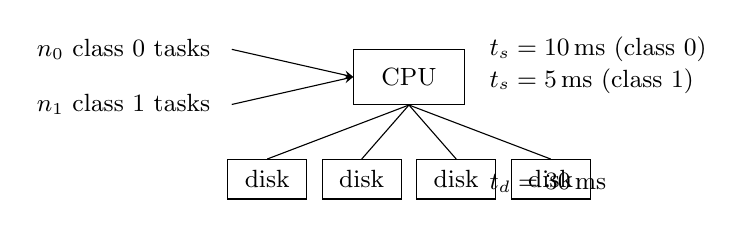
\begin{tikzpicture}[font=\small, line width=0.4pt, >=stealth]
  \node[draw, rectangle, minimum width=1.4cm, minimum height=0.7cm] (cpu) at (0,0) {CPU};
  \node[draw, rectangle, minimum width=1.0cm, minimum height=0.5cm] (d1) at (-1.8,-1.3) {disk};
  \node[draw, rectangle, minimum width=1.0cm, minimum height=0.5cm] (d2) at (-0.6,-1.3) {disk};
  \node[draw, rectangle, minimum width=1.0cm, minimum height=0.5cm] (d3) at (0.6,-1.3) {disk};
  \node[draw, rectangle, minimum width=1.0cm, minimum height=0.5cm] (d4) at (1.8,-1.3) {disk};

  \node[anchor=east] at (-2.4,0.35) {$n_0$ class 0 tasks};
  \node[anchor=east] at (-2.4,-0.35) {$n_1$ class 1 tasks};
  \draw[->] (-2.25,0.35) -- (cpu.west);
  \draw[->] (-2.25,-0.35) -- (cpu.west);

  \draw (cpu.south) -- (d1.north);
  \draw (cpu.south) -- (d2.north);
  \draw (cpu.south) -- (d3.north);
  \draw (cpu.south) -- (d4.north);

  \node[anchor=west] at (0.9,0.35) {$t_s = 10\,\mathrm{ms}$ (class 0)};
  \node[anchor=west] at (0.9,-0.05) {$t_s = 5\,\mathrm{ms}$ (class 1)};
  \node[anchor=west] at (0.9,-1.35) {$t_d = 30\,\mathrm{ms}$};
\end{tikzpicture}
\caption{Central Server Queueing Network}
\end{figure}

To see how the functions described in preceding sections are used, we'll look
at a high-level model of a hypothetical computer system. This system is
represented by the queueing network of Figure 2.1. Networks with this
structure are called central server networks.\footnote{Buzen's development of
efficient computational algorithms for analyzing central server queueing
networks [Buzen 1973] triggered a series of advances in queueing network
analysis methods.}

The system comprises a CPU and four disks. A fixed number of tasks of two
different classes execute in the system, alternating between CPU and disk
activities. There are $n_0$ class 0 tasks, which have a mean CPU execution time
of 10 ms., and $n_1$ class 1 tasks, which have a mean CPU execution time of
5 ms. CPU execution times for both classes are exponentially distributed. CPU
requests of class 1 tasks have preemptive priority over those of class 0 tasks.
If a class 1 task requests the CPU when it is being used by a class 0 task, the
latter is preempted and queued, and the CPU is assigned to the class 1 task.
The interrupted task resumes CPU execution when there are no more class 1
tasks requesting the CPU.

The disk requests of both classes are distributed randomly and uniformly
across all four disks, with the same mean disk service time of 30 ms. Disk
service times are assumed to be Erlang-distributed with a standard deviation
equal to 1/4 of the mean service time.

\paragraph{Open and closed systems.}
The M/M/1 queueing system simulated in Chapter 1 is an open system; customers
arrive from someplace outside the system, are serviced, and leave the system.
The source of customers presumably is unlimited: the probability of a new
customer arriving in the system is not influenced by the number of customers
already in the system, so queues in an open system potentially can grow
without limit. The central server queueing network is a closed system; tasks
receive service at the CPU, at a disk, and then recirculate to request service
at the CPU once again. (The time-sharing system of problem 4, Chapter 1, also
is a closed system.) The maximum queue length at any facility is bounded by
the number of tasks in the system. We can look at this closed network as
representing a fixed-level multiprogramming system with a queue of tasks large
enough so that, whenever a task leaves the system, it is immediately replaced;
the number of tasks executing in the system always remains the same.

Let's assume that the objective of the simulation is to estimate the mean tour
time, or cycle time, for each class. A tour time is the interval between two
successive CPU requests of a task. If we know the mean tour time of a class
and the mean number of tours it makes (mean number of disk requests), we can
compute the mean time a task spends in the system.

\paragraph{The simulation program.}
Figure 2.2 shows a smpl implementation of this model. smpl function names are
underlined in this figure. Preprocessor directives (lines 2--6) define the
number of tasks, the number of disks, and a symbolic representation (gd) for
the value returned by a request or preempt function when a facility
reservation request is queued.

Tokens, in this model, represent tasks. Lines 7--12 define a structure array
of task attributes: these are a task's class, the unit number for the task's
current IO disk request, and the starting time of its current tour. Token
values in smpl function calls in this model are indexes of the element of this
array. Note the array dimensioning: the first element is unused so that we
won't have a token with a 0 value.

The declarations of lines 13--19 define variables used to save descriptors
returned by facility definition functions, to specify the number of tours to be
simulated, and to hold CPU and disk service time distribution parameters.

The first statements of main() initialize variables used to accumulate tour
counts and times for each class. Line 24 sets the class of each task. Lines
25--28 are initialization operations common to all smpl simulation programs:
smpl() is called to initialize the simulation subsystem, facilities are
defined, and the initial events are scheduled. Note that the effect of this
last initialization step is to begin the simulation with all tasks scheduled
for event 1: the simulated system is otherwise empty. This probably is an
unusual system state; we would expect to find tasks distributed throughout the
system (unless there was a major ``bottleneck'' at some point). This state
will be reflected in measurement data collected during the first part of the
simulation run, biasing estimates of steady-state system performance.

\begin{figure}[ht]
\centering
\begingroup\small
\begin{verbatim}
#include <smpl.h>

#define n0 6      /* no. class 0 tasks */
#define n1 3      /* no. class 1 tasks */
#define nt n0+n1  /* total no. of tasks */
#define nd 4      /* no. of disks */
#define gd 1      /* queued req. return */

struct token {
    int cls;   /* task class (& priority) */
    int un;    /* unit for current IO req. */
    real ts;   /* tour start time stamp */
} task[nt+1];

int i, j, event, n[2];
real s[2];
int disk[nd+1], cpu, nts = 10000;
real te[2] = {10.0, 5.0}; /* class 0/1 mean CPU times */
real td = 30.0, sd = 7.5; /* disk time mean, std. dev. */

main()
{
    struct token *p;

    n[0] = n[1] = 0; s[0] = s[1] = 0.0;
    for (i = 1; i <= nt; i++) task[i].cls = (i > n0);

    smpl(0, "central server model");
    cpu = facility("CPU", 1);
    for (i = 1; i <= nd; i++) disk[i] = facility("disk", 1);
    for (i = 1; i <= nt; i++) schedule(1, 0.0, i);

    while (nts) {
        cause(&event, &i);
        p = &task[i];

        switch (event) {
        case 1: /* begin tour */
            p->ts = time();
            schedule(2, 0.0, i);
            break;

        case 2: /* request cpu */
            j = p->cls;
            if (preempt(cpu, i, j) != gd) then
                schedule(3, expntl(te[j]), i);
            break;

        case 3: /* release cpu, select disk */
            release(cpu, i);
            p->un = random(1, nd);
            schedule(4, 0.0, i);
            break;

        case 4: /* request disk */
            if (request(disk[p->un], i, 0) != gd) then
                schedule(5, erlang(td, sd), i);
            break;

        case 5: /* release disk, end tour */
            release(disk[p->un], i);
            j = p->cls;
            s[j] += time() - p->ts;
            p->ts = time();
            n[j]++;
            schedule(1, 0.0, i);
            nts--;
            break;
        }
    }

    printf("class 0 tour time %6.2f\n", s[0] / n[0]);
    printf("class 1 tour time %6.2f\n", s[1] / n[1]);
}
\end{verbatim}
\endgroup
\caption{Queueing Network Simulation Program}
\end{figure}

It is possible to devise more elaborate initialization schemes, but this is
seldom done because of the extra programming effort required. Usually we'll
either discard measurement data collected early in the run or make the run
long enough so that this initialization bias has negligible effects on
results. We'll discuss this problem at some length in Chapter 4.

The length of the simulation run is controlled by nts. When the program is
initialized, this variable is set to the number of tours to be simulated; it is
decremented on each tour completion (line 53) and tested by the while
statement of line 29. Simulation run lengths typically are controlled either
by specifying the simulation time period, as we did in the M/M/1 queue
simulation in Chapter 1, or by specifying an execution count for some
activity. (Also, for certain output analysis methods, runs are terminated when
a specified system state is reached.) Termination on count, rather than time,
is recommended since sample counts are needed in the statistical analysis of
simulation output. We'll usually have a better idea of how many samples we
need than of how much time it will take to collect them.

The cause() function call of line 31 gets the next event together with the
index of the task for which the event is to be executed. This event is then
used to select the appropriate event ``routine'' to execute. Note that a
pointer to the array element for the task is set on line 31.

Event 1 is the start of a tour; the current simulation time is saved as the
tour start time, and event 2 scheduled for immediate occurrence. Event 2
represents a task's CPU request. Remember that a task's class corresponds to
its priority in this model. The preempt() function call requests that the CPU
be reserved for this task. If the CPU currently is reserved by a task of the
same or higher priority, the request is queued, a queued response is returned,
and the event routine simply exited. If the CPU is free, it is reserved for the
requestor. If the CPU is busy with a lower-priority task, that task is
interrupted and queued, and the CPU then reserved for the higher-priority
task. Once the CPU has been reserved for the task, the end of its current CPU
execution interval (event 3) is scheduled. Note that the mean execution
interval is selected according to the task's class.

Two points from our earlier discussion of facility operations bear repeating
here. First, note that recording the tour start time and requesting the CPU
must be done in separate event routines. A blocked CPU request will be queued
and, when the CPU becomes available at some later time, event 2 will be
rescheduled for it. If the tour start time were to be recorded in the same
event routine in which the CPU request is issued, the start time would be
recorded twice: once on the initial CPU request and again on the request's
reexecution. Second, even though events 1 and 2 occur at the same simulation
time, transfer between the two event routines is done indirectly, via a
schedule() call, rather than directly. When cause() returns an event, it
records that event as the current event. If a CPU request is blocked, the
current event number -- event 2 -- is saved in the queue entry created for the
request and, when the CPU becomes available, event 2 is rescheduled. If
control is transferred directly between event routines, smpl loses track of the
current event.

Event 3 marks the completion of a task's CPU execution interval. The CPU is
released, a disk unit selected at random, and the disk request scheduled. If
there are requests queued for the CPU, smpl will dequeue the request at the
head of the queue and return it to execution. There are two possibilities. If
the request was a blocked CPU request, event 2 is scheduled for it at the
current simulation time; reexecution of event 2 will reserve the CPU for the
dequeued request. If the request was a preempted request, the CPU is reserved
for it by smpl, and event 3 is rescheduled for the request.

Event 4 represents the initiation of a task's disk request. (By now it should
be clear why selection of the disk unit and the request for that unit are in
separate event routines.) If the selected unit is busy, the request is queued;
otherwise, the unit is reserved for the requestor and the end of the disk
operation scheduled.

Event 5 is the completion of a task's disk request and of its current tour. The
disk unit is released, the time of the current tour is computed and added to
the accumulated tour times of the task's class, and the count of completed
tours for that class is incremented. The start of the next tour for this task is
scheduled, and the count of the number of tours to be simulated is
decremented. When this count reaches 0, the mean tour times for class 0 and
class 1 are computed and displayed. The values obtained using the random
number generator described in Chapter 8 are 99.34 and 69.37 ms.,
respectively.

Most of the smpl functions described earlier in this chapter are used in this
simulation program, so it is important to understand what the program does
and why it does it. Also, many models will have the same general form as this
one, perhaps with additional facility stages. Similar models are used in other
contexts; for example, the central server network of Figure 2.1 might
represent a memory bus and memory modules, rather than a CPU and disks.
(We'll look at simulation and analytic models of a multiprocessor memory
system in Chapter 5.)

To practice using smpl functions, you may want to try extending this model;
there are a number of possibilities. The level of detail of disk request
processing can be expanded by defining facilities to represent disk
controllers and data channels, decomposing the disk service time into seek,
latency, and transfer times, and adding event routines to initiate and
terminate these activities. The model can be extended to represent
transaction processing by adding an event routine to generate transaction
arrivals and dynamically allocating and deallocating task attribute array
entries as transactions arrive and depart.

\paragraph{A matter of style.}
The format of this and subsequent programs in this book differs in some
respects from common C usage. Differences include the use of then (defined as
empty in smpl.h) and the positioning of braces. This reflects only the
author's preference in program style and not any advocacy of style. In moving
the smpl source code in the Appendix to your system, you should feel free to
reformat it according to your own preference.

\section{Debugging Aids}
\label{sec:smpl-debugging-aids}

\paragraph{Error messages.}
Various errors are detected by smpl. When an error is detected, smpl displays
or prints an error message, generates a simulation report (if the current
output destination is the printer), and terminates simulation program
execution. Error messages give the simulation time at which the error was
detected and one of the following diagnostic clauses.

\begin{verbatim}
empty element pool
empty name space
facility defined after queue/schedule
negative event time
empty event list
preempted token not in event list
release of idle/unowned facility
stream argument error
uniform argument error: a > b
random argument error: i > j
erlang argument error: s > x
hyperx argument error: s not > x
\end{verbatim}

smpl maintains a common pool of elements from which the event list and data
structures for facilities and queues are constructed. The size of this pool is
fixed when smpl is compiled. An empty element pool error occurs when the
total number of static and dynamic entities for which pool elements must be
allocated exceeds the size of the pool. Sometimes this simply is due to the
size of the model, and the only cure is to increase the size of the pool. It
frequently is caused by a ``runaway'' simulation program which generates
arrivals but not departures. A second pool is used to hold model and facility
names; when this pool is filled, an empty name space error occurs. You can
shorten the names or increase the size of this pool.

An error occurs if a facility is defined after an event has been scheduled or a
facility request queued (for reasons which have to do with data structure
creation). Sequencing model operations in the required order will eliminate
this error.

Scheduling an event with a negative inter-event time usually results from some
kind of computation problem (but remember that variates from the normal
distribution can be negative).

An error occurs when cause() finds the event list empty, usually because a
scheduling operation was forgotten someplace (and sometimes because we've
unwittingly modeled a deadlock situation).

When a token's use of a facility is preempted by a higher-priority token, smpl
searches the event list to find an entry for the token being preempted. It
assumes that this entry represents the end of the token's execution interval
on that facility, and suspends the remaining part of the interval until the
facility is once again available for that token. An error occurs if the
preempted token can't be found in the event list. This usually results from a
program bug, but sometimes results from model complexities which exceed the
restrictions imposed by smpl's implicit queueing.

When a facility is released, smpl verifies that the token specified in a
release() call is the same as the reserving token: if it is not, an error
occurs. This catches a surprising number of program bugs.

The remaining errors in this list result from invalid arguments in random
number generator function calls and were described earlier.

The above errors result in calls to the smpl function

\begin{verbatim}
error (n, s);
int n; char *s;
\end{verbatim}

which also can be called from a simulation program. You may want to do this to
generate a simulation report on a program-detected error. In this case, n (an
error code used by smpl) should be 0, and s should point to a string
containing the diagnostic clause you want included in the error message. An
error message always is displayed on the screen; if the current output
destination is the printer, it also is printed, followed by the simulation
report. (Output destination control is described later on in this chapter.)

\paragraph{Traces.}
When the cause of an error isn't obvious from an examination of the program,
we can use the smpl trace to get additional information. Tracing is controlled
by calls to the following function.

\begin{verbatim}
trace (n);
int n;
\end{verbatim}

n, the trace control flag, should be in the range 0--4; any other value is
ignored. Values in the range 1--3 turn tracing on; a 0 value turns tracing off.

\begin{figure}[ht]
\centering
\begingroup\small
\begin{verbatim}
time 79.898 -- token 7 -- CAUSE EVENT 5
- token 7 -- RELEASE disk
- token 7 -- SCHEDULE EVENT 1
- token 7 -- CAUSE EVENT 1
- token 7 -- SCHEDULE EVENT 2
- token 7 -- CAUSE EVENT 2
- token 7 -- PREEMPT CPU: INTERRUPT
-- SUSPEND EVENT 3
-- QUEUE token 4 (inq = 3)
-- RESERVE CPU for token 7
- token 7 -- SCHEDULE EVENT 3

time 87.828 -- token 7 -- CAUSE EVENT 3
- token 7 -- RELEASE CPU
-- DEQUEUE token 4 (inq = 2)
-- RESERVE CPU for token 4
-- RESUME EVENT 3
- token 7 -- SCHEDULE EVENT 4
- token 7 -- CAUSE EVENT 4
- token 7 -- REQUEST disk QUEUED (inq = 1)

time 96.976 -- token 2 -- CAUSE EVENT 5
- token 2 -- RELEASE disk
-- DEQUEUE token 7 (inq = 0)
-- RESCHEDULE EVENT 4
- token 2 -- SCHEDULE EVENT 1
- token 7 -- CAUSE EVENT 4
\end{verbatim}
\endgroup
\caption{smpl Trace Message Sequence}
\end{figure}

If n is 1, the trace is free-running; trace messages are generated
continuously on the screen or printer, depending on the current output
destination. If n is 2, trace messages are sent to the screen; execution is
paused whenever the screen fills. If n is 3, trace messages also are sent to
the screen but with a pause after every message. In both cases, execution is
resumed following a pause by pressing any key. User trace messages can be
intermingled with smpl trace messages. After each user trace message is
displayed or printed, a trace(4) call will cause smpl to update line counts and
issue a page change or screen pause if appropriate.

When the error occurs early in the execution of our simulation program, we can
turn tracing on as part of model initialization and step through model
execution, screen by screen, until the error occurs. After we get the early
(and usually easy) bugs out, and encounter errors later in the simulation,
this approach becomes too time-consuming. We can add an event routine to our
simulation program which, when the corresponding event occurs, will turn
tracing on. During initialization, we schedule that event to occur some time
earlier than the error; how much earlier is a matter of guesswork -- the error
and its cause may be far apart in time.

When tracing is on, messages are generated whenever a facility is defined,
requested, or released, and whenever an event is scheduled or caused. Trace
messages give the time at which the operation occurred (if it has changed
since the previous trace message) and identify tokens involved in the
operation. Messages for schedule and cause operations give the associated
event number. Messages for facility request and release operations give the
facility name and the current queue length at the facility, and show the
queueing and dequeueing of tokens.

Figure 2.3 shows a sequence of trace messages from the execution of the
simulation program of Figure 2.2. This sequence traces the execution of a
token from the completion of one disk request up to its initiation of its next
disk request. This token -- token 7 -- represents a higher-priority (class 1)
task.

The trace sequence begins at the end of a tour for token 7: event 5 occurs, the
disk is released, and event 1 scheduled. There is no inter-event delay between
event 5 and event 1, so event 1 occurs immediately (event 1 simply records the
tour start time), and event 2 is scheduled. Again, there is no delay between
events 1 and 2, so event 2 occurs immediately. Event 2 is a CPU request. Since
the CPU is reserved by a lower-priority token, token 4, preemption takes
place. The event 3 scheduled for token 4 is suspended, token 4 is placed on
the CPU queue (whose length now becomes 3), and the CPU is reserved for token
7. Token 7 then schedules its release of the CPU, event 3. Note that all these
operations take place at the same point in simulation time.

In this particular sequence, there are no intervening events between events 2
and 3 of token 7. When its event 3 occurs, token 7 releases the CPU. Token 4,
which was interrupted earlier, is dequeued (reducing the CPU queue length to
2), the CPU is reserved for it, and its suspended execution interval resumed.
Token 7 schedules event 4 and, on its occurrence, issues its disk request. This
request finds the disk unit busy and is queued; note that it is the only
request queued for this unit.

The next event to occur is the completion of a disk request for token 2. When
this token releases the disk, token 7 is dequeued and event 4 rescheduled for
it. After token 2 has scheduled the start of its next tour, token 7's disk
request (event 4) is reinitiated.

smpl trace messages usually provide enough information to pinpoint problems in
simple simulation programs. However, while these messages can show which
operations are performed, they can't show why; as program complexity
increases, so does the need for user-level debugging aids. If you get involved
in developing large simulation models, build in debugging facilities from the
start.

SMPL debugging aids. SMPL provides several facilities to help speed debugging.
Simulation time is continuously displayed on the screen, and execution can be
paused at any time by pressing a key. For more precise control, a breakpoint
can be set from the keyboard to pause execution at a specified time or a
specified parameter value is reached. Tracing can be turned on and off via
function keys. SMPL provides a ``dump'' capability, which displays the state
of the simulated system, including facility status and users, queue entries,
and event list contents (an example appears in Section 7.4). The dump display
can be generated at any time from the keyboard; it also is generated whenever
an error occurs. The ability to control basic debugging aids from the keyboard
greatly reduces the amount of time spent modifying and recompiling simulation
programs.

\section{Data Collection and Reporting}
\label{sec:smpl-data-collection-reporting}

smpl collects data on facility utilization and queueing, and uses this data to
produce the simulation report. This report gives the utilization, mean busy
period, mean queue length, and release, preempt, and queue operation counts
for each facility. The reported measures represent operations completed from
the start of the current measurement interval up to the time of the report. The
measurement interval starts at simulation time 0 unless the reset() function
is called. reset() clears facility counters and accumulators, discarding
measurement data collected up to the time of its call, and sets the start of
the measurement interval to the current simulation time. The simulation report
is generated and sent to the current output destination by the following
function call.

\begin{verbatim}
report ();
\end{verbatim}

This function generates the simulation report and sends it to the current
output destination. Figure 2.4 shows the simulation report obtained by adding
a report() function call to the simulation program of Figure 2.2. The report
heading includes the model name, the current simulation time, and the
measurement interval length (which corresponds to the simulation period in
this case). Facility names are those specified in facility() function calls. In
this model, all facilities have single servers. For a multi-server facility,
the number of servers is appended in brackets to the facility name.

\begin{figure}[ht]
\centering
\begingroup\small
\begin{verbatim}
smpl SIMULATION REPORT

MODEL: central server model      TIME 29652.553

INTERVAL: 29652.553

MEAN BUSY   MEAN QUEUE   OPERATION COUNT
FACILITY     UTIL  PERIOD LENGTH   RELEASE PREEMPT QUEUE
CPU          0.8151 6.202 1.2286    12687   2682   7335
disk         0.7872 29.970 0.933    2484    0      1838
disk         0.7161 29.704 0.847    2457    0      1787
disk         0.7804 29.844 0.921    2514    0      1896
disk         0.7886 30.029 0.951    2939    0      1931
\end{verbatim}
\endgroup
\caption{smpl Simulation Report}
\end{figure}

The utilization of a facility is computed by dividing the accumulated busy
time of all servers by the length of the measurement interval; the
utilization of a multi-server facility may be greater than 1. Busy times are
accumulated when a server is released, so the utilization does not reflect
facility execution intervals in progress at the time of the report. This end
effect usually is insignificant because of the relative length of the run, but
should be kept in mind when using a report covering a small simulation period
in debugging.

The mean busy period is computed by dividing the accumulated busy time by the
release count. The release count is the sum of release operations effected via
a release() call and those resulting from facility preemption. For
non-preemptable facilities, the reported mean busy period should be
approximately equal to the mean facility execution interval specified in the
simulation program. Note that the mean disk busy periods in this report are
very close to the specified mean disk service time of 30 ms.

For preemptable facilities, the reported mean busy period is not necessarily
 the same as the mean execution interval, since it reflects interrupted
intervals. However, we can compute the mean execution interval from the
reported data. The product of the mean busy period and the release count (or
 the product of the utilization and the measurement interval) gives the total
busy time. The preempt count is the number of actual preemptions which
occurred, so the difference between the release count and the preempt count
is the number of completed execution intervals. Dividing the total busy time by
this number gives the measured mean execution interval.

Let's compare the measured mean CPU execution interval with that we'd expect
from the values specified in the simulation program. From the report data, the
mean interval is (6.202 x 12687) / (12687 - 2682) = 7.865 ms. The two classes
of tasks in this model have different mean CPU execution times; to compute an
overall mean, we need counts of the number of completed CPU execution
intervals for each class. We can obtain values very close to these counts by
adding statements to the simulation program to print the class 0 and class 1
tour counts, n[0] and n[1]. For this particular implementation, these are 5827
and 4173. The mean CPU times specified for class 0 and class 1 are,
respectively, 10 ms. and 5 ms., so we'd expect an overall mean of
(5827 x 10 + 4173 x 5) / 10000 = 7.914 ms. The measured mean of 7.865 ms. is
very close to this value.

The mean queue length of a facility is the average number of tokens in the
facility's queue; it does not include tokens in service. The mean queue length
is computed using the method described in Section 1.5. The mean number of
tokens in queue and in service at a facility is the sum of the facility
utilization and the mean queue length. The sum of utilizations and mean queue
lengths for all facilities is the mean number of tokens in the system (for the
report of Figure 2.4, the sum is 8.9994).

The release count is the sum of all facility releases, including those
resulting from preemption. The preempt count is the number of actual
preemptions (not the number of preempt() function calls). The number of
complete facility operations is the difference between the release count and
the preempt count. This number, divided by the measurement interval length,
is the facility's throughput. The average time in queue at a facility can be
computed by dividing the mean queue length by the throughput of the facility.

The queue count is the number of dequeue operations performed during the
measurement interval. It includes requests queued because the facility was
busy and requests queued after preemption. The difference between the queue
count and the preempt count is the number of blocked requests.

Sometimes you'll want to develop a report tailored to a particular model. The
U(), B(), and Lq() functions described in Section 2.4 (together with the
operational relationships discussed in Section 1.4) can help in doing this.

\paragraph{SMPL Reports.}
SMPL provides additional data collection and reporting tools. These include
the table facility, used to collect, tabulate, and plot distributions of model
variables, and the time series display, used to plot a variable such as average
or instantaneous queue length versus time. With SMPL, any report can be
displayed at any time simply by pressing a function key. We'll look at the
design of the table facility in Chapter 9.

\section{Output Control}
\label{sec:smpl-output-control}

Error and trace messages, and the simulation report, are sent by smpl to the
current output destination. This destination is initially set to stdout.
(Turning tracing on with a trace control flag of 2 or 3 also sets the output
destination to stdout.) You can redirect output to the printer or a disk file,
or find out what the current destination is, via a call to the following
function.

\begin{verbatim}
p = FILE *sendto (dest);
FILE *dest;
\end{verbatim}

If dest is null, sendto() returns the file pointer of the current destination.
If it is not null, the associated file becomes the current output destination.

\section{Summary}
\label{sec:smpl-summary}

This chapter has described the simulation, debugging, and reporting functions
of smpl, and discussed their use in a queueing network simulation program.
We'll look at more smpl simulation programs in Chapters 5 and 6. If you have
questions about any of these functions, read the appropriate section on
implementation in Chapter 8, or check the source code in the Appendix. The
simulation functions discussed in this chapter are summarized in Figure 2.5. A
few utility functions were not described here; you'll come across these in
moving smpl to your system. (When this move is accomplished, you can use the
program of Figure 2.2 as a test case. If you use the same random number
generator, you should be able to reproduce exactly the mean tour values, the
trace sequence, and the simulation report.)

If the subject of operational analysis (introduced in Section 1.4) is new to
you, it would be a very useful exercise to read Chapters 2 and 3 of Lazowska
et al.\ [1984] and apply the relationships discussed in these chapters to the
analysis of the output from this model. Go through the arithmetic to compute
throughputs, queueing times, and residence times at each facility, and for
 each class at the CPU. This may seem just a matter of bookkeeping (and in
some respects it is), but an understanding of these relationships is very
important in model development and testing, and sometimes will eliminate the
need to build a model at all.

\begin{figure}[ht]
\centering
\begingroup\small
\begin{verbatim}
INITIALIZATION

smpl (0, s)      initialize simulation subsystem
reset ()         clear measurement counters & accumulators

FACILITY DEFINITION, OPERATION, AND QUERY

f = facility (s, n)  define facility & return descriptor
r = request (f, j, p) reserve facility: r = 1 if queued
r = preempt (f, j, p) preempt facility: r = 1 if queued

release (f, j)   release facility & dequeue request
r = status (f)   get current facility status: r = 1 if busy
n = inq (f)       get current queue length
u = U (f)         get utilization
b = B (f)         get mean busy period
l = Lq (f)        get queue mean length

EVENT SCHEDULING

schedule (e, t, j) schedule event
cause (e, j)       cause event (e, j are pointers)
j = cancel (e)     cancel event & return token
t = time ()        get current simulation time

DEBUGGING AND REPORTING

trace (n)          set trace mode
error (n, s)       display error message & halt
report ()          generate simulation report

lcnt (n)           count output lines on current page
endpage ()         advance (pause) on full page (screen)
newpage ()         initialize page/screen line count
d = sendto (d)     get/set output destination

RANDOM VARIATE GENERATION

n = stream (n)     set/get random number stream number
v = ranf ()        generate uniform [0,1] variate
v = uniform (a, b) generate uniform [a,b] variate
v = expntl (x)     generate exponential variate
v = erlang (x, s)  generate Erlang variate
v = hyperx (x, s)  generate hyperexponential variate
v = normal (x, s)  generate normal variate
k = random (i, j)  generate random integer
\end{verbatim}
\endgroup
\caption{smpl Function Summary}
\end{figure}

\section{Problems}
\label{sec:smpl-problems}

\begin{enumerate}
\item Run the M/M/1 queue simulation model of Figure 1.7 and use the data
provided by the smpl simulation report to compute the system throughput $X$
and mean residence time $W$. Replace the server in this model by two servers
operating at one-half the speed of the original single server (doubling $T_s$),
run the revised model, compute $X$ and $W$ for this M/M/2 queue, and compute
the ratio of residence times for the two systems. (Both systems have the same
expected throughput $1/T_a$.) Increase the system load by reducing $T_a$ to
125.0, and repeat the two runs; what happens to the residence time ratio?

\item Extend the M/M/1 queue model of Figure 1.7 to provide a preemptive
priority queueing discipline. Assume there are two independent customer
classes: both have mean inter-arrival times of 400 units and mean service times
of 100 units, but class 2 customers have higher priority than class 1
customers. Implement some type of customer descriptor record so that arriving
customers can be marked with their class and arrival time; instrument the
model to compute and report the mean residence time for each class and for all
customers. Run this model using the same simulation period as the model of
Figure 1.7, and compare the values of $W$ obtained for the combined classes
with that obtained for the M/M/1 queue with first-come, first-served queueing.

\item A simple timesharing system model. A timesharing system (problem 4,
Chapter 1) has 16 user terminals connected to a computer system with two
identical disks. Figure 2.6 shows a queueing diagram of this system. Workload
characteristics are the same for all 16 users; user think times have a
negative exponential distribution with a mean think time $Z$ of 5 seconds.

Processing of a terminal request requires a mean CPU time of 480 milliseconds
(ms.) and an average of 12 disk requests. The mean CPU execution interval per
disk request therefore is 40 ms. Inter-disk-request intervals are
exponentially distributed. For modeling purposes, it can be assumed that, when
a disk request completes, another CPU execution interval is initiated with
probability $p_x$ or terminal request processing is completed (and another
think time initiated) with probability $1 - p_x$. $p_x$ is defined as
$1 - 1/n_{io}$, where $n_{io}$ is the average number of disk requests per
terminal request. ($n_{io} = 12$, then, in this case.)

Disk requests are distributed randomly, independently, and uniformly across
the two disks. The service time for a disk request is the sum of seek, latency,
and transfer times; data is transferred in units of one block (or sector).
Disks have a revolution time of 16.7 ms., a minimum seek time of 0 ms., a
maximum seek time of 50 ms., and a transfer time of 0.52 ms. per block. While
 the mean seek time is not known, observation indicates that most seek times
are in the vicinity of 16 ms., so it is assumed that the seek time distribution
can be modeled by a triangular distribution with range [0, 50] ms. and mode
16 ms. (see problem 3, Chapter 1). Latency times are distributed uniformly in
[0, 16.7] ms., and disk requests transfer one block of data.

\begin{figure}[ht]
\centering
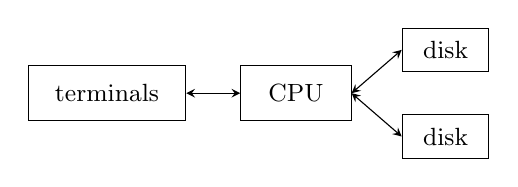
\begin{tikzpicture}[font=\small, line width=0.4pt, >=stealth]
  \node[draw, rectangle, minimum width=2.0cm, minimum height=0.7cm] (terms) at (-2.4,0) {terminals};
  \node[draw, rectangle, minimum width=1.4cm, minimum height=0.7cm] (cpu) at (0,0) {CPU};
  \node[draw, rectangle, minimum width=1.1cm, minimum height=0.55cm] (d1) at (1.9,0.55) {disk};
  \node[draw, rectangle, minimum width=1.1cm, minimum height=0.55cm] (d2) at (1.9,-0.55) {disk};

  \draw[<->] (terms.east) -- (cpu.west);
  \draw[<->] (cpu.east) -- (d1.west);
  \draw[<->] (cpu.east) -- (d2.west);
\end{tikzpicture}
\caption{Timesharing System Queueing Diagram}
\end{figure}

Build a smpl model of this system, instrumenting the model to collect terminal
request response times and to report the mean response time. All queues have
first-in, first-out queueing. Make a simulation run of 2000 terminal requests
and perform an operational check of the results, using utilizations and queue
lengths from the smpl simulation report to verify the mean response time.
Determine the mean number of terminal requests in the system.

\item Representing memory. The above model has no provision for representing
the effect of memory capacity on response time. The simplest way to represent
memory is to assume that the system has a multiprogramming level (mpl) of $m$
active users. When a terminal sends a request to the system, that request is
accepted by the system and its execution initiated if the number of requests
currently being executed is less than $m$; otherwise, the system queues the
request until one of the $m$ executing requests complete. Assume the system
has a mpl of 6, and add memory queueing to your model. (One possibility is to
represent memory as a facility with 6 servers.) Make a simulation run of 2000
terminal requests and perform an operational analysis of the results. Compute
the response time components: memory waiting time, mean CPU residence time per
terminal request, and mean disk residence time per terminal request. Compare
the mean response time and mean number of requests in the system with those
obtained for the model of problem 3.

\item Representing swapping. The work performed by a user at a terminal in
this system involves a continuing series of interactions between the user and a
program executing in the computer system. Each user interacts with a different
program (or, equivalently, with a different instance of a common program). To
execute, a program requires memory and certain logical resources which,
collectively, are called an address space. It is assumed that the
multiprogramming level, or mpl, specifies the number of address spaces in the
computer system.

The program assigned to a given address space is said to be resident.
Resident programs have two states: active and dormant. A program is active
while executing and dormant when it has completed execution and returned a
response to the terminal. When the system receives a terminal request, it
determines if the user's program is resident. If it is, the program is
scheduled for execution. If it is not, and there is an address space
containing a dormant program, the system swaps out the dormant program to disk
and swaps in the requested program to that address space.

Extend the model of problem 4 to represent swapping, based on the following
assumptions. The computer system has 6 address spaces. (These can be
represented by a facility with 6 servers; a server is reserved when the
program in an address space becomes active and released when the program
becomes dormant.) When a terminal request arrives for a non-resident program
and all address spaces contain active programs, the request is queued until one
of these programs becomes dormant and an address space can be assigned to the
request. The system then swaps out the dormant program and swaps in the
program being activated. If a request for a non-resident program finds several
address spaces with dormant programs, it swaps out the program which has been
dormant the longest.

The number of disk blocks transferred by a swapout is assumed to be
distributed uniformly between 30 and 60. The system chooses a swapout
destination disk at random; if the chosen disk is busy, the swapout is
assigned to the other disk regardless of that disk's status. The number of
blocks and source disk for a program's swapin are established when the
program is swapped out. The operating system serializes swap operations so
that only one swap, in or out, is in progress at any one time by placing
swapout and swapin requests on a FIFO queue. (A smpl facility can be used to
represent this queue.) If a terminal request arrives to find its program being
swapped out to accommodate an earlier arrival, the swapout is allowed to
complete. If an address space is available, it is assigned to the
newly-arrived request and a swapout initiated for the dormant program in that
address space. Since swaps are serialized, the swapin of the program for this
request will not be initiated until its swapout completes.

Make a simulation run of 2000 terminal requests. Compute the response time
components as before (keep in mind that swap queue delays and disk transfers
for swapouts do not contribute to the response time except when a program
swapin has to wait on its own swapout).

\item Incorporating CPU scheduling. Suppose terminal requests are classified,
more or less arbitrarily, as class 0 or class 1, depending on whether their CPU
time requirements are less than or greater than 250 ms. Instrument the model
of problem 5 to report response times by class, as well as the overall response
time.

\begin{enumerate}
\item Some systems use round-robin (RR) CPU scheduling so that a request for a
small amount of CPU time will not be disproportionally delayed by execution of
a request requiring a large amount of CPU time. With RR scheduling, the CPU is
cyclically allocated to the requests in the CPU queue. Each request, in turn,
receives CPU service for a fixed quantum of time (or for the time remaining in
its current execution interval, if smaller than a quantum). Incorporate RR
scheduling in the model of problem 5, using a quantum time of 25 ms. Simulate
2000 terminal requests. Compare the results with those obtained in problem 5.
What effect did the incorporation of RR scheduling have? Why?

Note that if your version of smpl uses 16-bit ints, the large number of CPU
operations required in simulating this system with RR scheduling will cause
some counters associated with the CPU facility to overflow, so that some
reported CPU measures will be meaningless. To circumvent this, generate a
simulation report and reset smpl after every 32767 CPU releases, and merge the
reports by hand at the end of the run. Alternatively, use the U(), B(), and
Lq() functions to get facility measures after every 32767 CPU releases, and
write a function to merge and report these measures.

\item Suppose the system attempts to favor class 0 requests by computing CPU
request priority based on accumulated CPU time as follows:

\begin{verbatim}
priority = max(0, 10 - [0.01 * accumulated CPU time])
\end{verbatim}

where [x] denotes the floor function of x -- the largest integer equal to or
less than x. Thus, a request is assigned a priority of 10 upon arrival, and its
priority is reduced by 1 whenever it accumulates another 100 ms. of CPU time
until it has been reduced to 0. Incorporate this scheduling algorithm into the
model of problem 5 (no RR scheduling) and simulate 2000 terminal requests.
Compare the mean response time of class 0 requests with that obtained without
priority scheduling. What can be done to improve the response time of class 0
requests? How would you model the proposed improvement?
\end{enumerate}
\end{enumerate}

% OCR draft from PDF pages 83-113. Needs cleanup and verification.
\chapter{Model Development and Testing}
\label{chap:model-development-testing}

\section{The Modeling and Analysis Process}
\label{sec:modeling-analysis-process}

This and the following chapter discuss the steps involved in developing and
using a simulation model. The key step in this process is that of abstracting
 a system design into a model design. No amount of discussion of this task can
take the place of experience, and even the experienced modeler finds new
challenges in each new system. The sooner you translate your interest in
simulation into experience, the better! It is useful to spend some time
building simulation models of queueing systems with known analytic solutions
 to become familiar with smpl, to develop simulation programming skills, and
to gain experience with the output analysis methods discussed in the next
chapter. To develop skills in abstracting from system design to model,
though, requires working with an actual system. It is best to begin with an
existing system with which you're familiar, and for which data can be obtained
for workload characterization and model validation. Start with a simple model:
if possible, select a modest subsystem that can be isolated from the rest of
the system. Picking a modeling subject in advance of reading this chapter will
help establish a context for the discussion which follows.

The modeling and analysis process is outlined in Figure 3.1. (The nice linear
flow shown in this figure rarely happens in practice; we'll usually go through
several iterations of parts of this process.) The process can be divided into
three phases: development, testing, and analysis. This chapter is concerned
with the development and testing phases.

The first step in development is describing system operation from a
performance viewpoint. This description then is abstracted, in accordance
with the objectives of the analysis, into a model description. This specifies
the facilities to be represented in the model and their interconnection, the
work to be represented and its attributes, and the operations involved in
accomplishing this work. The level of the detail of the model determines the
data to be collected. Next, the appropriate analysis method is chosen, and a
model implementation is developed. We'll assume this takes the form of a
simulation program; alternatively, it could involve translating the model
design and data to input parameters for a queueing network analysis package.

The testing phase comprises three steps: debugging, verification, and
validation. All too often, the simulation program is considered to be
debugged when it runs to completion without errors and produces
``reasonable'' results: single-server facility utilizations are between 0 and 1,
and so on. Verification insures that the simulation program is indeed an
implementation of the model. Validation insures that the model is a
reasonable representation of the real system.

\begin{figure}[ht]
\centering
\begin{tikzpicture}[font=\small, node distance=0.6cm]
  \tikzstyle{flowbox}=[draw, rectangle, minimum width=9.0cm, minimum height=0.7cm, align=center]
  \node[flowbox] (sd) {SYSTEM DESCRIPTION};
  \node[flowbox, below=of sd] (sa) {SYSTEM ABSTRACTION \& MODEL DESCRIPTION};
  \node[flowbox, below=of sa] (dc) {DATA COLLECTION};
  \node[flowbox, below=of dc] (am) {ANALYSIS METHOD SELECTION};
  \node[flowbox, below=of am] (spd) {SIMULATION PROGRAM DEVELOPMENT};
  \node[flowbox, below=of spd] (dbg) {PROGRAM DEBUGGING};
  \node[flowbox, below=of dbg] (ver) {VERIFICATION (program vs. model)};
  \node[flowbox, below=of ver] (val) {VALIDATION (model vs. system)};
  \node[flowbox, below=of val] (soa) {SIMULATION OUTPUT ANALYSIS};
  \node[flowbox, below=of soa] (pa) {PROBLEM ANALYSIS};

  \draw[->] (sd) -- (sa);
  \draw[->] (sa) -- (dc);
  \draw[->] (dc) -- (am);
  \draw[->] (am) -- (spd);
  \draw[->] (spd) -- (dbg);
  \draw[->] (dbg) -- (ver);
  \draw[->] (ver) -- (val);
  \draw[->] (val) -- (soa);
  \draw[->] (soa) -- (pa);
\end{tikzpicture}
\caption{The Modeling and Analysis Process}
\end{figure}

\section{System Description}
\label{sec:system-description}

We've generally assumed that the designer and modeler are the same person.
When they are different persons, the modeler's first task is learning how the
system works and describing its operation from a performance viewpoint; this
description provides the basis for developing a model. The modeler relies on
the designer to provide the knowledge needed. If the two fail to communicate,
the analysis effort is, at best, a waste of time; at worst, it can result in bad
design decisions. Communication problems can be both technical and
inter-personal.

Effective technical communication places responsibilities on both designer and
modeler. The designer has a broad view of the system: the modeler, a narrow
one. However, the modeler has to learn enough about the design to determine
what aspects are critical to its performance and must be included in the
model. The designer and modeler are mutually responsible for the latter's
education. The modeler needs to gain both a working knowledge of the overall
design and a detailed understanding of the part of the system to be modeled.
He has to understand this part in more detail than he plans to model it. The
designer has a continuing responsibility for answering questions about design
details; because the modeler's view differs from the designer's, these
questions may cut across design levels and modules. The modeler needs to
explain to the designer what analysis results can be expected, why particular
questions are being asked, and how the answers will be used. The design may
be incomplete (for reasons motivating the analysis in the first place), and
designer and modeler need to work together to develop the assumptions needed
to carry out the analysis.

The learning process is difficult enough when designer and modeler have a
good working relationship; it becomes almost impossible if there are
inter-personal difficulties. Rightly or wrongly, the burden of avoiding these
usually falls on the modeler. At the start, he has to show that he has
assimilated all available information on the design project and avoid asking
questions any dumber (from the designer's viewpoint) than necessary. Notes of
answers to questions should be kept, so questions don't get asked twice. The
modeler has to work to establish rapport with the designer and demonstrate
the ability to contribute to the design. He has to be very clear about what he
can and cannot do; otherwise, the first mistake will destroy his credibility.
Above all, the modeler has to be sensitive about publicizing results;
broadcasting performance problems is certain to harm future communication.

The knowledge the modeler gains in this learning process is an abstraction of
 the design, a model in its own way, and reflects a number of assumptions,
some explicit, some implicit. The modeler's view of how the system operates
should be documented, this system description reviewed by the designer, and
any appropriate revisions made. When the designer agrees with the
description, it becomes an informal contract between designer and modeler.
The designer usually will let the modeler know when design changes affect this
description, and will readily accept results from models based on it. The time
spent in organizing and writing this description will be more than compensated
for by the errors it eliminates. The form of this description depends on the
type and scope of the system being modeled; it may be nothing more than a
one-page flow diagram.

\section{System Abstraction and Model Description}
\label{sec:system-abstraction-model-description}

A model is an abstraction of a system, and represents a particular view of
that system. Models frequently are described in terms of the method used to
obtain performance measures: analytic model, simulation model, measurement
model. (The last describes taking a certain level of view of actual system
operation and collecting data at that level.) At this point in the modeling
and analysis process, we want to develop a representation of the system which
captures its essential performance-determining characteristics. We should not
develop this representation with a particular analysis method in mind; if we
do, we can easily and unconsciously introduce invalid assumptions. What we
want to do is describe what is to be represented in the model: choosing an
analysis method comes later.

A model description of a simple system typically takes the form of a diagram
showing system resources (both hardware and software) and their
interconnection, annotated to show the flow of work through the system and
the operations involved, and accompanied by explanatory notes and
descriptions of assumptions. It identifies decisions and timings dependent on
attributes of work as well as timings dependent only on the system design. For
complex systems, multiple levels of diagrams may be used to show the
configuration, and flow charts or pseudo-programs used to describe processing
operations. Its style depends on the design background of the modeler
(hardware or software) and on his analysis orientation (e.g., queueing
networks); the way in which it is developed depends on how the abstraction
process is approached.

There are no formal rules for abstracting a system design into a model
description. Our simulation texts are no help in this area, and our
performance texts don't offer much more. Approaches differ from problem to
problem (and person to person), but basically either employ synthesis or
 decomposition.

\paragraph{Synthesis.}
Synthesis begins at the level of the design description. To form a higher-level
description, elements of the system are combined (or perhaps just ignored),
and associated activities are correspondingly combined and simplified. In
making each simplification, we need to ask ourselves if and how we've
preserved the essential underlying characteristics. Have we adjusted the
processing time of the higher-level activity? If we've combined resources,
have we properly accounted for delay times? What is the possible impact on
the distribution of processing times? Each simplifying assumption should be
recorded; those which make us nervous should be marked for later
investigation. The synthesis process may take several steps, each creating a
higher level of description. When the desired level of detail is reached, we
should review all the assumptions made and assess their probable impact on
the results of the analysis. If the net effect is likely to be optimistic (or
pessimistic), now is the time to make a note of it; it's easy to lose sight of
it in later stages.

\paragraph{Decomposition.}
Decomposition is the reverse of synthesis. The system initially is viewed as a
single entity, its work viewed at the highest level (computer system, job; disk
subsystem, request; LAN, message). Work is decomposed into its principal
activities, the system into the set of resources used by these activities; this
process is repeated through increasing levels of detail until the desired level
is reached. In decomposition, we start with very general assumptions and
refine them in advancing from one level of detail to the next. We may be less
at ease with some of these than equivalent assumptions arrived at by
synthesis: the step-by-step construction of the latter seems a stronger basis.
On the other hand, we may feel that decomposition provides a better overall
representation; we can always add detail if we're in doubt. Again, we need to
note our assumptions and estimate how they might bias the results. In either
approach, the strongest assumptions probably will be very much the same, and
will involve describing work.

Which approach should you choose? Sometimes you won't have a choice: it'll be
dictated by the design approach. Sometimes a synthesis approach seems obvious
because of your knowledge of the system; at other times, the workload data
available determines the approach. Large systems are best approached via
decomposition. If the choice seems open, use decomposition: it is better to
begin at a high level of abstraction and add detail later than to begin with
too much detail.

There are several advantages to an iterative decompositional approach in which
a series of models, each of increased detail, is developed and analyzed. It is
easier to uncover cause-effect relationships in higher-level models than in
very detailed ones; this may shorten the analysis effort. A higher-level model
is useful in verifying a lower-level model; a high-level analytic model can be
the principal means of verifying a lower-level simulation model. Hierarchical
development of a model blends nicely with a stepwise refinement approach to
simulation program development.

Maintaining a roughly uniform level of detail at any given level of
description supports a hierarchical development of the model. However, the
final model may reflect several levels of detail, particularly when the
analysis focuses on a particular subsystem. This target subsystem is
represented at the level of detail needed to satisfy analysis objectives; other
subsystems are modeled primarily to establish an operating point for this
subsystem, and can be represented in less detail.

One last note. There are two ways we can view a system and its work: we can
view work as operating on the system, or we can view the system as operating
on the work. In high-level models, we usually take the first view. For
example, in a high-level model of a computer system, we think of jobs or tasks
as reserving and releasing facilities and allocating and deallocating memory.
The system is viewed only in terms of static entities; its dynamic components
-- operating system processes, in this example -- are lumped together with the
work, rather than explicitly represented. This is fine at a high level of
abstraction, but there is a limit to its decomposition. If we try to carry it
too far, we'll end up building one awkward construct after another, and we'll
lose similitude between model and design. In developing a highly detailed
model, it is better to take, at the very start, the view that the system
operates on its work and explicitly represent the dynamic entities, as well as
 the static entities, of the system.

\section{Data Collection}
\label{sec:data-collection}

When development of the model description is complete, we'll have a good idea
of the kind and level of detail of data we need to ``drive'' the model. The
next task is to list the model parameters which have to be specified
numerically and determine their values. These parameters can be categorized
as workload parameters (such as inter-arrival times, execution times, storage
requirements, record types and lengths) and system parameters (usually timings
for various operations, such as the memory cycle time). A parameter may have
a single fixed value, or it may have to be specified in terms of the
 distribution of its values.

It's useful to start by determining values of system timing parameters; the
requisite analysis of the system may show that some of these are functions of
workload parameters and result in additions to our list. When modeling an
existing system, it may be possible to measure parameters either directly
(via hardware or software instrumentation) or indirectly (via regression
analysis). When modeling a design, parameter values will have to be estimated
(they are rarely over-estimated).

Determining values of workload parameters and, in particular, specifying
distributions, is the hardest part of the analysis process. Measurement and
characterization of actual system workloads can provide values directly to the
analysis of existing systems, and can provide a basis for estimating values for
use in analyzing new systems. Workload characterization is a subject in its
own right and outside the scope of this book; unfortunately, it also seems to
be outside the scope of most performance evaluation books. The best single
reference on computer system workload characterization (at the job or task
level of view) is Ferrari et al.\ [1978]; the methods and considerations
 discussed in this book can be applied in other subject areas. Ferrari's
earlier book [Ferrari 1978] also is useful. A review of conference proceedings
and technical periodicals in your area of interest may turn up some useful
information, although papers on workload characterization are an order of
magnitude less frequent than papers on analysis. The subject doesn't lack
importance -- it just has a high work-to-glory ratio.

It is difficult to carry out a workload characterization study of a particular
environment, and extremely difficult to study a range of environments. The
difficulties increase with the level of detail with which the system is
viewed. In undertaking a study, we'll often find that existing measurement
tools are inadequate, and that collection of the data we need requires adding
instrumentation to the system. This may not be possible; even when it is, the
added overhead or added risk may limit its use so that studying a range of
environments is impossible. The data that we do collect can present a variety
of analysis challenges, and it is difficult to substantiate any claims of
representativeness. The difficulties in doing a good job of workload
characterization aren't an excuse for its circumvention, but rather emphasize
the need to allocate adequate resources and time to it in planning performance
studies.

While there is no substitute for the insights gained from studying actual
system behavior, blind use of measurement data -- because it's ``real'' -- can
create a false sense of confidence in the analysis and its results. We need to
be careful first in extrapolating from the measurement environment to the
analysis environment and second in drawing conclusions about results. In
working with real systems, it is very hard, and frequently impossible, to
demonstrate that a design performs as desired: the universe of work is too
large to fully explore. However, it only takes one data point in that universe
to demonstrate that a design doesn't perform. If an analysis based on workload
measurements indicates a performance problem, we'll probably be very confident
that the design doesn't work. However, if the analysis doesn't indicate a
problem, we won't be equally confident that the design does work. The
confidence we do have will be a direct reflection of our confidence in the
workload characterization process.

We'll often have to undertake an analysis even though we have very little data
 to work with. If we can estimate a ``reasonable'' set of parameter values, and
an analysis based on these values finds a problem, we've earned our keep.
However, if it doesn't, we haven't proved anything; we'll have to estimate a
range of values for each parameter, and carry out additional analyses. Because
of the number of combinations of parameters, we may do sensitivity analyses
 to identify those which significantly affect results. Other tactics include
specifying parameter values to obtain worst-case or best-case results. We may
be able to arrive at reasonable assumptions about the means or ranges of
parameter values. However, in the absence of insight from measurements, it is
difficult to make equally reasonable assumptions about distributions. (Some
of the considerations in choosing a distribution are discussed in Section
1.2.) The sensitivity of results to distributional assumptions can be
analyzed, but the number of data points involved limits how much of this can
be done. Often all we can do is worry -- with justification.

Shortage of data provides added motivation for an iterative approach to the
modeling and analysis process. There's not much point in refining model
assumptions beyond those we have to make about parameters. A higher-level
model requires fewer (although broader) assumptions than a more detailed
model. If we do find a performance problem using a higher-level model, we've
saved development effort. If we don't, a higher-level model, particularly one
that can be evaluated analytically, speeds sensitivity analyses.

As we collect data and specify the values of the parameters on our list, we
should make careful notes of the assumptions made. Using these assumptions,
we may be able to derive an exact analytic result for our model or, if we use
simulation, provide a tight confidence interval for a result. In either case,
``exactness'' of results doesn't compensate for looseness of assumptions --
something we need to remember when we print our results to three decimal
places!

\section{Analysis Method Selection}
\label{sec:analysis-method-selection}

The choice of an analysis method is based in part on the required system and
data representations, and in part on our tools and skills. We always should
try arithmetic first; if an operational analysis shows that some facility is
110\% busy, we don't need to carry the analysis further. In some cases, we can
estimate performance bounds; if the lower bound on response time exceeds our
design goal, we're done with the analysis for the time being.\footnote{Lazowska
et al.\ [1984] describe computation of performance bounds for batch-, terminal-,
and transaction-oriented computer systems; their approach can be adapted to
other problem contexts. Stuck and Arthurs [1985] give numerous examples of
performance bounds estimation.} When further analysis is needed, the model
description is translated into an analytic model or a simulation model.

\paragraph{Analytic versus simulation methods.}
In following the technical literature on performance evaluation, you'll come
across this comparison now and again. The phrasing may lead you to believe
that, as a simulation modeler, you are lacking in purity and grace. In doing
performance analysis in a real-world design environment, what counts is
function, not form. The best method is arithmetic: beyond that, the choice
depends on your particular skills and how effective you are in applying them.
Successful performance analysis uses both methods, and uses them together.
Only fools and angels don't check analytic results against simulation.
Simulation models are used as submodels of analytic models, and conversely, in
hybrid modeling, and analytic models can be used in simulation model
verification.

\paragraph{Choosing a method.}
We'll always choose an analytic model when one exists that fits our model
description, even when the next iteration in model development requires
simulation, because of its solution speed and because we can use it in
verifying the simulation model. We may be able to use a commercial queueing
network analysis package. (However, the assumptions and approximations used
in these packages may not be documented, and we need to be careful in trying
to use them outside their intended application range.) If an appropriate
analytic model does not exist, we may develop one if time and skill permit, or
perhaps we can adapt a model found in the technical literature.

The choice frequently is one of either making further simplifying assumptions
in order to use an analytic model or developing a simulation model. If the
analytic approach doesn't require a lot of effort, we'll go ahead with it in
any case; it may identify a performance problem, and we can use the results in
simulation model verification. Deciding whether or not to develop a simulation
model depends on how critical we think these assumptions are and on the effort
required. If the effort is modest, we'll develop the simulation model anyway
and use it to check the analytic results as well as the effects of the
additional assumptions.

\section{Hybrid Modeling}
\label{sec:hybrid-modeling}

Hybrid modeling combines analytic and simulation modeling. It is particularly
useful when a model represents processes whose execution rates differ by
orders of magnitude. A common example is a model of job execution in a
computer system, where each job may execute from tens to thousands of IO
requests. An analysis of job performance might require simulation of several
thousand jobs to achieve the desired level of confidence; this would
necessitate simulating hundreds of thousands of disk requests, and the
resulting computational cost would be prohibitive. Schwetman [1978] and Chiu
and Chow [1978] solve this problem via a hybrid modeling approach. A
simulation model is used to generate job arrivals and make job-level
scheduling decisions; a queueing network model is used to determine how long
 each job executes. To examine their approach, we'll look at a simple hybrid
model of computer system job scheduling.

The objective of this model is assumed to be the evaluation of a scheduling
policy which, on the basis of a job's memory requirements, determines when to
admit a job into execution. The simulation and analytic model components of
this hybrid model are illustrated in Figure 3.2. The simulation model operates
only at the job level, and represents just two events: job arrivals and job
completions. The analytic model (in this example, a simple central server
model) represents the compute and disk activities of active jobs.

\begin{figure}[ht]
\centering
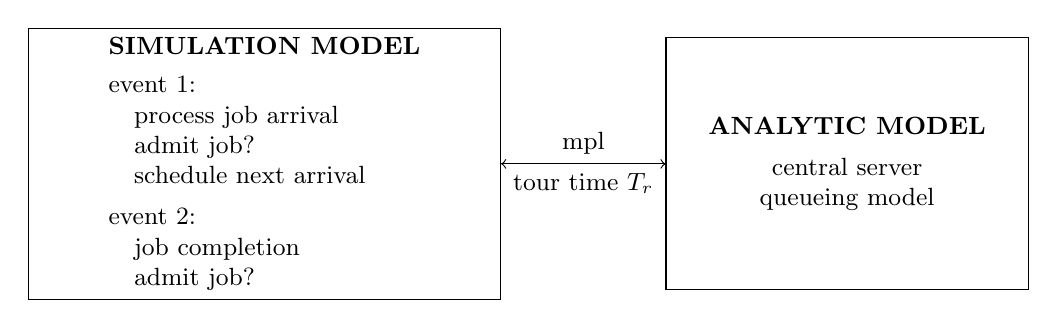
\begin{tikzpicture}[font=\small, line width=0.4pt]
  \node[draw, rectangle, minimum width=6.0cm, minimum height=3.2cm, align=left] (sim) at (-3.7,0)
  {\textbf{SIMULATION MODEL}\\[0.3em]
   event 1:\\
   \quad process job arrival\\
   \quad admit job?\\
   \quad schedule next arrival\\[0.4em]
   event 2:\\
   \quad job completion\\
   \quad admit job?};

  \node[draw, rectangle, minimum width=4.6cm, minimum height=3.2cm, align=center] (ana) at (3.7,0)
  {\textbf{ANALYTIC MODEL}\\[0.4em]
   central server\\
   queueing model};

  \draw[->] (sim.east) -- node[above] {mpl} (ana.west);
  \draw[->] (ana.west) -- node[below] {tour time $T_r$} (sim.east);
\end{tikzpicture}
\caption{Simulation and Analytic Components of the Hybrid Model}
\end{figure}

The simulation model generates arrivals, determines when a job is to be
admitted into execution, computes job completion times, schedules job
completions, and accumulates performance measurement data when jobs complete.
It computes the next job completion time by finding the job with the smallest
number of CPU-disk tours remaining, invokes the analytic model to determine
the mean tour time, and computes how long that number of tours will take. To
compute the mean tour time, the analytic model requires mean CPU and disk
service times, disk routing probabilities, and the number of jobs executing
(i.e., the multiprogramming level, or mpl). For simplicity, we'll assume that
mean service times and routing probabilities are the same for all jobs and are
established when the model is initialized. Consequently, the analytic model
only needs the current mpl to compute the mean tour time. Note that, if
desired, we could change the service times and routing probabilities of the set
of active jobs as jobs enter and complete execution.

The event routines and functions of the simulation model component are
outlined in Figure 3.3. arrival is caused when a job arrival event occurs. It
generates the attributes of the job, enters the job in the admission queue,
schedules arrival of the next job, and calls the job scheduling function to
determine if the job can be admitted to execution. One of the attributes
generated for a job is the number of CPU-disk tours to be executed.

The job scheduling function, job\_schedlr, is called whenever a job arrives or
leaves the system. It scans the admission queue for a job which satisfies the
rules of the admission policy. If such a job is found, update is called to
update tour counts (since placing another job in execution will change the mean
tour time). update calls the solve function to evaluate the analytic model and
compute the mean tour time. The time elapsed since the last update is divided
by the mean tour time to determine the mean number of tours completed since
then, and the tour counts of the active jobs are decremented by that number.
job\_schedlr then dequeues and activates the selected job and increments the
multiprogramming level. Increasing the number of jobs in execution will affect
tour times, making the scheduled next job completion event invalid, so it is
cancelled (it also is possible that the newly-activated job may complete
execution before any other job). The next\_completion function is called to
schedule the next completion. Although not shown in the outline of Figure 3.3,
the scheduling function should go on to try to activate additional jobs, since
completion of one job might free enough memory space to permit several jobs to
enter execution.

The next\_completion function scans the set of active jobs to find the one with
the smallest number of tours remaining. It invokes the analytic model to
determine the mean tour time, computes the remaining execution time for that
job by multiplying the number of tours by the mean tour time, and schedules
completion of that job.

The completion event routine is ``caused'' when a job completion event occurs.
It updates tour counts, deactivates the completed job (i.e., deallocates its
job descriptor table entry), and accumulates job performance measures, such as
the time spent in the system. It calls next\_completion to schedule the next job
completion, and calls the job scheduling function to see if jobs in the
admission queue can now be activated.

Job measures such as the mean system residence time and the mean number of
jobs in the system are computed using the methods described in Sections 1.4
and 1.5. Performance measures for entities of the analytic model are computed
by collecting measures for each inter-update interval and weighting them
 either by the relative interval length or relative number of operations in the
interval. (As a practical exercise in applying operational analysis, try
working out the computation of overall throughput, utilization, mean queue
length, and mean residence time for the CPU.)

\begin{figure}[ht]
\centering
\begingroup\small
\begin{verbatim}
arrival event routine
  generate job attributes:
    ... memory requirements
    ... no. of tours (Nt)
  job -> admission queue
  schedule next arrival
  call job_schedlr
  cause next event

job_schedlr function
  return if no job satisfies admission rules
  call update
  dequeue & activate selected job
  mpl += 1
  cancel currently-scheduled completion
  call next_completion
  return

update function
  call solve to compute mean tour time (Tr)
  compute mean no. of tours completed since last update (n)
  decrement tour counts (Nt) of all active jobs by n
  return

next_completion function
  find active job (job i) with smallest no. of tours
  call solve to compute mean tour time Tr
  schedule job i completion: te = Nt(i) * Tr
  return

completion event routine
  call update
  deactivate job, accumulate job performance measures
  mpl -= 1
  call next_completion
  call job_schedlr
  cause next event
\end{verbatim}
\endgroup
\caption{Hybrid Model Event Routines and Simulation Functions}
\end{figure}

Hybrid modeling can provide substantial savings in computation time. In our
example, there are only two events per job (ignoring cancelled events) and
only two events in the event list at any time, so the simulation part is very
fast. The analytic model has to be evaluated only on job activation and
completion. The number of arithmetic operations required for its exact
solution is proportional to the product of the multiprogramming level and the
number of servers, and this should be small compared with the number required
 to simulate a job's disk requests. Even faster solutions can be obtained using
approximation methods. Schwetman [1978] compared hybrid and simulation models
of several systems, and reported CPU time improvement factors ranging from 18
 to 200. The improvement for a particular model depends on the relative
complexity of the analytic model and the simulation model it replaces.

Hybrid modeling is not applicable in every situation. The analytic model
usually requires stronger assumptions than the simulation model it replaces,
and this won't always be acceptable. The hybrid model discussed here adds the
assumption that the use of mean, rather than actual, tour times does not
significantly affect job residence times. This assumption is based on the
notion of decomposability in the sense used by Courtois [1977] (alternatively,
see Courtois [1975]). However, when the main functions of some parts of a
model are to establish an operating point for or provide work to the key part
of the model, the assumptions associated with these supporting parts often are
less critical. In such cases, it may be possible to replace a set of
simulation operations by an analytic function.

Given, for example, an analytic function for the distribution of operation
times, we can use the distribution's inverse to generate random operation
times. Sometimes a set of operations can be represented by a graph model whose
parameters (execution times, branching probabilities) are determined by
simulation. Rather than explicitly simulating these operations and scheduling
each execution time, it may be possible to obtain the mean overall execution
time and variance using analytic reduction methods (see Beizer [1978] or
MacDougall [1975]). Depending on model assumptions, this mean can be used as
the operation time, or the mean and variance can be used to generate a sample
operation time from a distribution. Some beforehand experimentation is needed
to determine the distribution's form.

Hybrid modeling is not discussed in any of the referenced simulation texts,
and receives only limited notice in most performance evaluation texts. Most of
the useful reference material has appeared in the form of technical conference
and journal papers. Schwetman's work (cited earlier) provided much of the
impetus for current work in this area. Chiu and Chow [1978] describe its
application to a complex computer system model. Shanthikumar and Sargent
[1983] divide hybrid models into four classes, discuss each class, and give
several examples of hybrid modeling. Blum et al.\ [1984] present experimental
comparisons of hybrid, analytic, and simulation models, and discuss advantages
of and problems in decomposition. Thomasian and Gargeya [1984] describe a
two-phase procedure for modeling a memory-constrained timesharing system with
 two customer classes. In the first phase, an analytic model is used to compute
system throughputs for the possible combinations of customers; these
throughputs are input parameters for the second phase, which uses a
simulation model to estimate mean response times. O'Reilly and Hammond
[1984] describe an approach to local area network modeling in which some
stations in the network are represented individually via simulation while the
remaining stations are represented collectively by an analytic model. This is
not a complete list; other examples can be found by reviewing the technical
literature in your area.

\section{Simulation Program Development}
\label{sec:simulation-program-development}

Developing a simulation program is very much like any other program
development task, although the quasi-concurrent nature of simulation program
execution sometimes gives it an operating system flavor. The main
considerations are

\begin{itemize}
\item simulation model design
\item program organization
\item parameter management
\item debugging aids
\item instrumentation
\end{itemize}

We'll discuss the first three topics in this section; debugging and
instrumentation are discussed in later sections.

\paragraph{Simulation model design.}
After deciding upon simulation as the analysis method, the next step is to
transform the model description into a simulation model design. This is -- or
at least should be -- the first point in the modeling process at which the
simulation language's view is imposed on the model. Our language is
event-oriented, so the model design defines sequences of activities with their
initiating and terminating events. However, if the model is complex, we
should try to approximate a process-oriented view by developing separate
definitions for different classes of processes (where a process can be a job, a
 task, or a request). This essentially involves defining a separate
 event-oriented model for each class and specifying any inter-model
coordination required (in addition to that provided by facilities). In
designing this model, we should try to maintain as much resemblance between
it and the system design as is reasonable at the model's level of abstraction.
(This similitude of model and system doesn't guarantee model validity, but is a
great help in achieving it.) As we outline activity and event sequences, the
data used at each step is identified and data structures developed for each
process class. A manual simulation of the final design can help catch errors
of omission.

\paragraph{Program organization.}
The next transformation is from model design to program design. The
organization of the program depends on the complexity of the model. For
simple models with few activities, the simulation program may look much like
those of Figures 1.7 and 2.2 -- a single procedure with events identified by
number. For somewhat larger models, we'll probably use separate function
procedures for each event routine and define events symbolically for easier
program modification. For complex model designs, where we've defined separate
models for each class of process, the program is organized as a set of
submodels, each of which may comprise a set of function procedures. (There is
 a limit on how complex a model we should attempt using smpl or any other
event-oriented language.) Some submodels may be combined at this point
(perhaps just to reduce code volume) in which case their data structures have
to be merged and modified.

Organizing the simulation program as a set of submodels representing different
process classes is facilitated by smpl's implicit queueing. Individual
submodels can execute independently, performing any necessary coordination
via operations on facilities. Explicit queueing would require that submodels
operate directly on one another. In modeling process coordination mechanisms,
smpl facilities can be used to represent such diverse entities as a hardware
flip-flop controlling a buffering operation or an operating system semaphore.
This representation range is somewhat limited by the inability to dynamically
create and destroy facilities (although smpl could be extended to provide
this).

The events defined in the simulation model design may be split or may be
combined into simulation program event routines. An activity initiation event
may have to be split into two event routines when it involves facility
reservation, since a blocked facility request results in reexecution of the
event routine which issued the request. Statements which should not be
reexecuted, such as those selecting the facility to be reserved or the token
involved in the operation, should be placed in a separate event routine (for
the reasons discussed in Section 2.4).

When an event representing the end of one activity and an event representing
 the initiation of another activity occur at the same instant in simulation
time, some code and execution time can be saved by combining both events in
one event routine. There are several things to consider before doing this. If
the event routine contains a facility request, reexecution of the routine
following a blocked request will cause problems. When the two activities
belong to logically different classes and the events coincide simply because
one activity freed a resource needed by the other, the loss of structure
resulting from combining event routines may not be worth the slight gain in
efficiency. Even when the activities belong to the same class and are
logically connected, debugging and expandability considerations may make
separation of event routines worthwhile.

For complex models, a top-down iterative approach to simulation model
development and programming is recommended. In this approach, the model is
initially defined at a high level of abstraction, comprising a small number of
macroscopic activities, perhaps defined only in terms of their execution
times. The level of detail of the model and the program are advanced in a
series of steps. At each step, (only) one activity of the model is refined into
a more detailed representation, and the simulation program is revised,
debugged, and verified at this new level of detail. At any point in model
development, the simulation program is executable and verifiable; each advance
in the level of detail can be checked against the preceding level.

\paragraph{Parameter management.}
Assigning values to model parameters is one of the more tedious aspects of
simulation program development. We have to decide which parameters we want to
assign values to from outside the program (i.e., at run time) and which will
be assigned values within the program (at compile time). Usually we will
considerably under-estimate the number of parameters we'll want to vary at run
 time.

There is one commandment for specifying parameters within the program: don't
``hardwire'' numeric values in the code. If we do, we'll inevitably have to
change them and, with equal inevitability, we'll miss one. The C macro
facilities are very helpful in this regard, not only in defining simple
symbolic constants but also in doing things like switching random variate
sampling functions.

Simulation program size and use determine how much effort to expend in
developing capabilities for run time input of parameter values. A large number
of parameters, or program use by other than the developer, justify a certain
amount of sophistication in the way of an input language as well as some error
checking. The development effort required can be surprising. In some large
simulation programs, one-third of the code is input processing, one-third is
report generation, and a modest one-third represents the model itself.
However, even the smallest model is much more convenient to use if an input
processor is provided, and we might as well implement it at the start, rather
than waiting until we get tired of recompiling. SMPL provides facilities for
defining and labeling input and output parameters, assigning input parameter
values either from the simulation program or from a display, and reporting
output parameter values (see Chapter 7). These facilities, although simple,
have proved to be very useful.

Defining values of compile-time parameters and providing input facilities for
specifying values of run-time parameters doesn't completely solve the
parameter management problem; we also need to tabulate parameter values as
part of model output. If we don't, we'll frequently find ourselves staring at a
simulation report and wondering under what conditions the results were
obtained.

\section{Simulation Program Debugging}
\label{sec:simulation-program-debugging}

Debugging is the task of getting the simulation program to the point where we
think it works -- it runs without errors and the results it produces seem
reasonable. Verification is the task of proving, as best we can, that the
program is a valid implementation of the model.

The tools used in simulation program debugging are the traditional ones: error
diagnostics, traces, dumps, and reports, all blended with a judicious
sprinkling of print statements. smpl error messages, traces, and reports were
 described in Chapter 2. SMPL adds a dump capability which shows the contents
of the event list and queues, and the status and users of each facility. You
may want to add a similar capability to your version of smpl (an example
appears in Chapter 7).

For small models, the standard smpl debugging aids, perhaps supplemented by
user trace messages and print statements, usually are adequate. Large models
should have trace, dump, and other debugging aids designed into the program
from the start. These should provide a logical view of model operation. To
control the volume of output, they should provide selectable levels of detail
for selectable parts of the model. Particular attention should be given to
model data structures: errors often occur in the dynamic allocation and
deallocation of token attribute records, particularly in the management of
associated indexes and pointers.

The procedure outlined below has proven to be efficient in the early stages of
program debugging.

\begin{enumerate}
\item On the first successful compilation of the program, try executing it.
Maybe it will run the first time out; in any event, we need to get the notion
out of our system!

\item Set up the simulation program to execute a single token, turn tracing
on, and trace the execution of this token. Review the trace data and the
simulation report to determine if the program executed correctly. It should be
straightforward to locate any problems.

\item Now revise the setup to execute two tokens sequentially (so that
execution of the second token can't begin until execution of the first token
completes), and again trace and review token execution. The objective is to
find problems left behind by the first token, such as facilities that didn't
get released, data elements that didn't get deallocated, and so on. Printing
values of pointers and indexes can help identify problems.

\item Revise the program once again to execute two tokens concurrently, trace
token execution, and look for problems in the interaction of the two tokens.
It may be necessary to initiate execution of the two tokens at the same time
to insure that queueing, preemption, or other resource conflicts occur. Verify
the flow of each token from event to event: problems in event routine
organization, such as unplanned reexecution of statements, often show up as
breaks in this flow.

\item Expand on this controlled execution process if the model is complex. For
example, the program can be modified to direct tokens along specific execution
paths, or to examine limit conditions such as communication network node
blocking on a packet limit. Sometimes the process can be simplified by
isolating submodels (or simply sections of the model) and driving them
independently.

\item When selective execution no longer turns up errors, try full execution
of a modest number of tokens. Watch the trace awhile to see if queues build up
because facilities aren't getting released. If a simulation error occurs, note
the time of its occurrence. Add an event routine to the simulation program to
turn tracing on, and schedule this event to occur some time earlier than the
error. (With SMPL, this can be done by setting breakpoints from the keyboard.)
How much earlier is a matter of guesswork: cause and effect may be widely
separated in time. The errors initially found at this step frequently are
caused by ``end game'' problems: conditions reached for the first time in
program execution, such as allocation of the last element in a free element
list.

\item When the model runs to completion without errors, review the simulation
report. Look at utilizations, queue lengths, and distributions of requests
across facilities to see if the values make sense intuitively and if they are
consistent in an operational analysis sense. In some cases (e.g., more than
one token class), this analysis may require adding instrumentation on the
simulation program. If the results are operationally correct but
counter-intuitive, find out why: there may be an error in service time
computation or an unanticipated (but perhaps valid) delay situation.
\end{enumerate}

In the personal computer arena, several C tools are available which could be
used to advantage in simulation program debugging; these include debugging
environments and C language interpreters. Another tool which has been
occasionally useful in debugging is the SMPL time series display (see Chapter
6). This display can be used to plot facility utilization, instantaneous or
average queue length, or a specified parameter value, versus time. When things
go awry at some point during execution without an error being detected, the
effects sometimes can be seen in the queue length display.

\section{Verification}
\label{sec:verification}

When the program produces reasonable results, debugging can be considered
complete (at least until a parameter change or use of a different random
number stream turns up another error), and we can turn our attention to the
next problem: verifying that the simulation program is a valid implementation
of the model. For small models, this may be obvious from inspection; for larger
models, some substantiating analysis is needed.

At a minimum, verification requires a comparative ``walkthrough'' of the model
description and the simulation program. Sometimes this is all that is
feasible, and success of the analysis effort depends on how diligently it is
done. However, additional verification via comparison with analytic models
often is possible. The simulation program is modified to represent a model for
which analytic results can be obtained, and the simulation and analytic results
are compared. This analytic verification does not, of course, guarantee that
the program matches the model. However, it does provide a way to eliminate
errors in at least part of the modeling process. If analytic verification is
successful, then any remaining errors are either in transforming the model
description to a model design or extending assumptions from the analytic model
to the simulation model.

A careful review is the only means of verifying the transformation of model
description to model design; however, since analytic verification involves
both simulation and analytic model design, it provides some cross-checking.
The extensions from analytic model to simulation model (suppressed for
verification) may take various forms, including distributional assumptions,
added level of detail, queueing disciplines, and token classes and priorities.
Although it may not be possible to analytically verify these extensions in the
context of the complete model, it may be possible to isolate parts of the
model and verify them independently. Sometimes a subsection of a closed system
model can be verified by isolating it and treating it as an open system model,
adding the necessary event routines to generate arrivals and handle
departures. In any case, extensions should be informally checked as part of
the process of returning the simulation program to its original form. We'll
often have some idea of what the effect of a changed assumption should be, and
can at least check to see that results change as expected. For example, if we
changed a distribution from hyperexponential to exponential for purposes of
verification, we would usually expect to see queueing increase when the
distribution was restored to a hyperexponential one. If we isolated part of
the model and verified that part in an open system, we would expect its
queueing delays to decrease when it becomes part of a closed system with a
finite number of customers.

The work involved in analytic verification can be reduced substantially by
planning for it at the start -- providing parameters to control extensions,
and developing, debugging, and verifying the model hierarchically. The only
hazard in this is a tendency to bias model development toward verification,
rather than application.

Where do we find analytic models to use in verification? For a variety of
single-queue, single- and multi-server open queueing systems, closed-form
expressions for expected values of parameters such as mean queue length and
residence time can be found in several of the referenced texts, in particular,
Allen [1978] and Kleinrock [1975]. Less extensive coverage appears in Banks
and Carson [1984], Kobayashi [1978], and Trivedi [1982]. Both Allen and
Kobayashi present results for the simplest closed queueing system, the machine
repair model. A simple algorithm for solution of central server queueing
systems was devised by Buzen [1973]; these systems are discussed in Kobayashi,
Trivedi, and several other texts. Ferrari [1983] provides a comprehensive
discussion of Buzen's algorithm, including load-dependent servers, and
includes a Fortran implementation of a central server model for computer
system analysis. However, the central server model is just a particular form
of queueing network; algorithms for the solution of more general network forms
are available. Lazowska et al.\ [1984] provide Fortran programs for the
solution of single job class and multiple job class networks. These are useful
in their own right for the task we're considering here; using the techniques
and algorithms described by Lazowska et al., these programs can be tailored
and extended as required in a particular application environment, and are
useful in analysis as well as verification. Finally, in addition to general
analytic models, specific analytic models from the technical literature can be
useful in verification, particularly when they have been validated.

The results obtained from simulation rarely, if ever, will agree exactly with
those obtained analytically. Simulation is a sampling process; in a simulation
experiment, we generate a large number of sample values and use the sample
mean as an estimate of the actual mean. Consequently, some difference between
simulation and analytic results can result from sampling variation. If this
 difference is small, we may not worry about it. Alternatively, we can carry
the analysis further: collect additional data, compute confidence limits for
the simulation estimate, and determine if these limits include the analytic
result. (This output analysis process is discussed in the next chapter.) For
reasons discussed in the next section, we should not expect to see comparable
percentage differences for all measures.

Another possible source of variation between analytic and simulation results is
approximations used in the analytic model. If the analytic model is one we've
developed ourselves, we are at least aware that approximations are used, and we
may be able to ``back off'' to an exact solution. If we're using a queueing
analysis package of some kind, result variations can be hard to interpret.
Package solution methods and use of approximations often are considered
proprietary and are not documented. (However, problems usually arise only when
the package is used differently than intended.)

\section{Validation}
\label{sec:validation}

Validation is the task of demonstrating that the simulation model is a
reasonable representation of the actual system: it reproduces system behavior
with enough fidelity to satisfy analysis objectives. The question of how much
is enough can be answered only in terms of these objectives and perhaps the
results obtained in the current iteration of the analysis process. For
example, demonstrating that a model tracks real-system trends may be
sufficient in a comparative analysis in which one alternative significantly
outperforms the other. On the other hand, when a critical system parameter
must be estimated within a few percent, the simulation model must be
demonstrably capable of providing that accuracy. The simulation model usually
is developed to analyze a particular problem and may represent different parts
of the system at different levels of detail. The model doesn't have to be
equally valid for all parts of the system over the full spectrum of system
behavior; it just has to meet the requirements of the problem.

The subject of validation gets terse treatment in our simulation texts. Of
these, Banks and Carson [1984] provide the best coverage, followed by Law and
Kelton [1982]. The discussion and references in Sargent [1984] provide a good
starting point for reviewing the literature. Balci and Sargent [1982] provide
a bibliography indexed by validation technique and by the statistical
technique used to compare measurement data and model results. Schatzoff and
Tillman [1975] and Teorey [1975] describe validations of computer system
simulation models. Schatzoff and Tillman illustrate the use of experiment
design methods and probability plots in simulation model validation; Teorey
presents a procedure for validation and illustrates it by application to an IO
subsystem model.

For purposes of this discussion, there are two different cases of validation to
consider. In the first case, the system being modeled exists and can be
measured, the analysis objective is to evaluate a proposed change to the
system, and validation is based on comparison of model results with
measurements. In the second case, the system being modeled exists only as a
design, and the analysis objective is to estimate performance of the design or
perhaps to evaluate alternative designs; little or no comparative data exists,
and validation mostly is a matter of design-model comparison.

\paragraph{Validation of models of existing systems.}
In this case, measurements of the existing system are compared with results
from a simulation of the existing system; if they agree, it is assumed that a
simulation of the modified system will produce valid estimates of the effects
of the proposed change. It all sounds so simple! The only problems are
measurement, comparison, and extrapolation.

Collecting system performance measures for use in validation ideally is done
when collecting workload characterization data. Conceptually, we want to
collect workload data over some period of operation, collect system
performance measures over that same period, drive the simulation model with
the workload data, and compare model results with measurements. Practically,
this can be hard to do. Measurement tool limitations can make it difficult to
match workload and performance data: for example, work in execution at the
beginning and end of the measurement period may not be properly accounted
for, and lengthening the measurement period is not always a solution.
Available performance measures may be incomplete, inconsistent or overlapping,
and not at the desired level of detail.

A number of measurement problems can be avoided or at least identified in
advance by developing a measurement model of the system. The measurement
model is derived from the analysis model description. It defines the
measurements and measurement points required for a complete description of
system performance, in an operational analysis sense, at the desired level of
detail. While it may not be feasible to instrument the system to provide these
measures, this model provides a framework to evaluate and apply available
measurements. The objective is to try to match these measurements to those
defined in the measurement model, adjusting the measurement points defined in
the model and the level of detail of parts of the model if necessary but
maintaining completeness if at all possible. (The difficulties in doing this
emphasize the need for something better than the usual ad hoc approach to the
design of system measurement facilities.) The final version of the measurement
model itself is validated by comparing aggregated workload data with traffic
and utilization measures.

Once the measurement model has been developed, the simulation model's
instrumentation should be revised or extended to report the same performance
measures as the system. Measures can be reported in the form of means, means
and variances, or distributions. While we can instrument the simulation model
 to provide any form, system measurement facilities often limit the forms in
which measurement data can be reported. Because of both reporting limitations
and statistical considerations, comparison of measurements and model results
generally is based on mean values.

The only test we can apply to a comparison of mean values from one measurement
period with means from one simulation run is a subjective one: how close are
the values? Except for trace-driven models, the work performed by the
simulated system and by the actual system are the same only in a statistical
sense; differences in measurement and model values arise because of sampling
variation as well as because of simplifying assumptions made in modeling. In a
subjective comparison, we rely on our judgement to determine if the values are
``close enough.''

In making this comparison, we shouldn't expect the same percentage difference
for all measures. To see why, consider an M/M/1 queueing system. The mean
number of customers in this system can be defined in terms of server
utilization as follows:

\begin{equation}
L = \frac{U}{1-U}
\end{equation}

The percentage change in $L$, $P_L$, resulting from a percentage change of
$P_U$ in $U$ can be obtained via differentiation:

\begin{equation}
P_L = \frac{P_U}{1-U}
\end{equation}

For example, at a base utilization of 0.5, a five percent change in
utilization translates into a ten percent change in the mean number in the
system. Consequently, a difference in measurement and model facility
utilizations can result in a larger difference in measures such as queue
length and response time, independent of all other effects. The magnifying
factor of the second equation applies only to the M/M/1 queueing system. It
will be smaller for some systems (e.g., systems with limited population or
lower service time variance) and larger for other systems; in most practical
cases it won't be explicitly known.

Other subjective validation methods include comparison of distributions. If
measurement facilities permit reporting the distribution of values of, for
example, system residence time, we can instrument the model to produce a
corresponding distribution, and compare -- by inspection -- the two
distributions. (A statistical comparison is not possible because the sample
values forming these distributions are not independent.) If the tails seem
significantly different, remember that they may represent only a few sample
values. The SMPL table facility (see Chapter 9) can be used to collect,
tabulate, and plot distributions of simulation data; it can also be adapted for
use in post-measurement data reduction.

Statistical techniques for comparing measurement and simulation results are
discussed in the references cited earlier in this section. In the simplest
case, multiple simulation runs are made to obtain the sample mean and sample
standard deviation for the simulation value, and a $t$ test used to decide if
the results are ``close enough.'' This is easy to do and we often want to
compute confidence intervals for simulation results anyway, as we'll discuss in
 the next chapter. In other cases, multiple sets of measurements are required,
and the additional data collection effort can pose problems unless planned in
advance.

We'd like to validate the model over a range of operating conditions broad
enough to encompass the planned analysis. (Doubling the validation points from
one to two will much more than double our confidence!) However, doing this --
particularly collecting the required measurement data -- can be costly. A
formal method for analyzing experimental cost versus the risk of accepting an
invalid model has been proposed by Balci and Sargent [1981], [1982]. While the
method may be outside the scope of the studies envisioned here, the discussion
of validation hypotheses is worth reviewing.

When the difference between measurements and simulation results is more than
we're willing to accept (or able to rationalize), we face a chore called
(euphemistically) model calibration. At some point in the modeling process, we
made a mistake. Most often it will be one of omission and will result in model
values being less than measured values. The problem may be an invalid
simplifying assumption. This assumption may have been made implicitly, so --
 in addition to checking explicit model assumptions against the system -- we
need to review system operation to see if we've left something out. Close
comparison of measurement and model data may provide some clues, as when queue
lengths agree in one part of the system but not another; this can result in a
quest for additional measurement data. Sometimes the problem is in data
collection: for example, operating systems often provide inadequate and
incomplete measurements of overhead time. In this case, the modeler is faced
with the temptation to ``calibrate'' (diddle) the model by adjusting model
input parameters to obtain output values which match the measurement data. (It
is hard to throw the first stone here.) Trying to find out why measurements and
model results don't agree can be very frustrating. It also can be very
rewarding, because it frequently provides new insights into system behavior.

When the model has been accepted as a valid representation, it is revised --
very carefully -- to represent the proposed change, and a new set of
simulation results are obtained and compared with those for the existing
system. Typically, the revised model uses the same set of workload parameters
as the validated model; we assume that the workload is unaffected by the
change. This assumption warrants examination: all systems are closed systems
with feedback effects if we look far enough. Although we may have only been
able to validate the original model at one or two points, we often want to
compare outputs of the original and revised models over a range of input
parameter values. Our confidence in the validity of analysis results depends
on the extent of the difference between the original and revised systems, and
will be higher for results obtained close to the validation points.

\paragraph{Validation of models of designs.}
When the system being modeled does not exist, validation primarily is done by
review; the model is examined in terms of the system design, and each
assumption and abstraction scrutinized and justified. This needs the
involvement of other design team members as reviewers, critics, and
contrarians; satisfying an expert audience is the best test of the validity of
model design and of system timing value assumptions. Workload parameter values
usually are determined by extrapolation from past systems. The design team's
review of these usually is based on judgement and experience, rather than on
the factual knowledge used to compare model and system designs: it may be
helpful to augment their review with one by knowledgeable system users.
Workload representativeness always is a concern; when the objective of the
analysis is an absolute prediction of the performance of the design, it is a
 key concern. When the objective of the analysis is a relative comparison of
design alternatives, we may be able to satisfy it using workload parameters
which are ``reasonable'', although not necessarily representative (see the
discussion in Section 3.4).

Similitude between system design and model is a key factor in validation. The
more the model resembles the design, the more likely is it to be valid, and
the easier it is for the reviewing designer to understand how the model
represents the design. Similitude is one aspect of what our simulation texts
refer to as ``face validity''. Correspondence of the simulation model to the
system design is guaranteed by a synthesis of design specification and
simulation model: ``the simulation is the design'' (Randell 1968). Simulation/
design synthesis is outside our scope: see MacDougall [1975] for a brief
discussion and additional references.

The two cases of validation described here represent ends of a spectrum. A
major change to an existing system presents much the same problem as a new
system design. Our confidence in a model of a new design is increased if we
can at least validate the approach with a similar model of an existing system.
In practice, validation often is blended with verification. If comparison of
measurements and model results is successful, then the simulation program is
assumed to be both a valid implementation of the model design and a valid
representation of the system. In modeling a new design, comparisons of
simulation program versus model design and of model design versus system
design tend to be done concurrently.

The final step in validation takes place when the system change is made or the
system design implemented, and predicted and actual performance can be
compared. This, unfortunately, doesn't happen very often in practice. The
final implementation may differ from the original design for reasons not
related to performance, and, in any case, the modeler is busy with a new
project and has little interest in auditing old work. In a system design
environment, there seldom is much pressure to carry out validation studies;
once the analysis has been done and the design decision made, alternatives are
discarded and the system gets built. The model becomes of historical interest
only, so few modelers ever pay for their sins. However, you will never know
how good or bad your analysis was unless you validate its results by
comparison with system measurements.

\section{Problems}
\label{sec:model-development-problems}

\begin{enumerate}
\item Estimating performance bounds sometimes eliminates the need for more
elaborate analysis and, in any case, provides a way of determining that our
simulation results are at least sensible. For a timesharing system such as that
of problem 3, Chapter 2, Lazowska et al.\ [1984] give asymptotic bounds for
throughput and response time.\footnote{Another method of bounds analysis called
balanced system bounds was developed by Zahorjan et al.\ [1982], and is
discussed by Lazowska et al.\ Balanced system bounds are ``tighter'' than
asymptotic bounds, and so are more useful for checking simulation results. The
discussion of bounds analysis in Chapter 5 of Lazowska et al.\ is recommended
reading.} The validity of these bounds depends only on the assumption that the
service time of one terminal request does not depend on the number or location
of other requests.

Let $D_k$ be the mean service demand (time) of a terminal request at server
$k$. Define $D = \sum D_k$ as the sum of the service demands of a request for
all $K$ servers, and define $D_{\max} = \max(D_1, D_2, \ldots, D_K)$ as the
largest service demand for any server. $X$, $R$, and $Z$ denote the
throughput, response time, and think time.

Consider throughput first. With a single terminal, there are no delays and the
throughput is $1/(D+Z)$. With $N$ terminals, the throughput is at best
$N/(D+Z)$, assuming no request ever has to wait for another request. At worst,
 each request finds $N-1$ requests ahead of it, and incurs a delay of
$(N-1)D$, and the throughput is $N/(ND+Z)$. Since a (single) server cannot
have a utilization of greater than 1, throughput is limited by the server with
the largest service demand to $1/D_{\max}$. The resulting bounds on $X$ are
shown in Figure 3.4(a).

The response time for a system with a single terminal is $D$. In the best
case, no request ever is delayed by another, and the response time continues
equal to $D$ as $N$ increases up to the point at which the utilization of the
busiest server reaches 1. At this point and beyond, the throughput is limited
 to $1/D_{\max}$ and, by the Response Time Law, the response time from this
point on is $N D_{\max} - Z$. In the worst case, each request has to wait a
 time $(N-1)D$ for other requests and so has a response time of $ND$. Figure
3.4(b) shows the bounds on $R$.

\begin{figure}[ht]
\centering
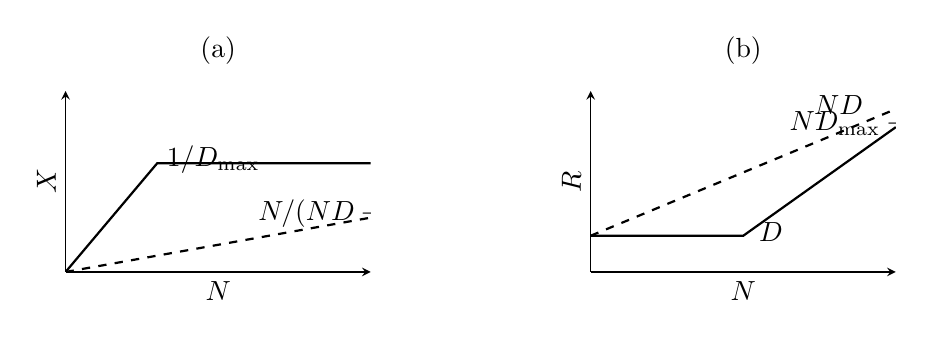
\begin{tikzpicture}
\begin{axis}[
  width=0.45\textwidth,
  height=0.32\textwidth,
  xlabel={$N$},
  ylabel={$X$},
  title={(a)},
  axis lines=left,
  xmin=0,
  ymin=0,
  xmax=10,
  ymax=1,
  ticks=none
]
  \addplot[thick] coordinates {(0,0) (3,0.6) (10,0.6)};
  \addplot[thick,dashed] coordinates {(0,0) (10,0.3)};
  \node[anchor=west] at (axis cs:3,0.62) {$1/D_{\max}$};
  \node[anchor=west] at (axis cs:6,0.32) {$N/(ND+Z)$};
\end{axis}
\begin{axis}[
  at={(0.55\textwidth,0)},
  anchor=origin,
  width=0.45\textwidth,
  height=0.32\textwidth,
  xlabel={$N$},
  ylabel={$R$},
  title={(b)},
  axis lines=left,
  xmin=0,
  ymin=0,
  xmax=10,
  ymax=10,
  ticks=none
]
  \addplot[thick] coordinates {(0,2) (5,2) (10,8)};
  \addplot[thick,dashed] coordinates {(0,2) (10,9)};
  \node[anchor=west] at (axis cs:5.2,2.2) {$D$};
  \node[anchor=west] at (axis cs:6.2,8.2) {$ND_{\max}-Z$};
  \node[anchor=west] at (axis cs:7,9.2) {$ND$};
\end{axis}
\end{tikzpicture}
\caption{Asymptotic Bounds for a Timesharing System (schematic)}
\end{figure}

Plot the throughput and response time bounds for the timesharing model of
problem 3, Chapter 2 for $N$ in the range 1 to 24. Locate the throughput and
response time values obtained from simulation on this plot. Assume that the
CPU in this system is replaced by a CPU of twice the speed, and plot response
 time bounds again.

\item The bounds described above can be applied to a ``batch'' system such as
that of Figure 2.1 by setting $Z$ to 0. Assume that, for any $N$, the
proportion of class 0 and class 1 tasks is the same as that in the model of
Figure 2.3. The CPU time per tour is the weighted sum of the class 0 and class
1 CPU times. The per tour service demand for a given disk is the product of
the visit ratio for that disk and the mean service time of that disk. The visit
ratio is the number of requests for that disk divided by the number of
requests for all disks, measured over an arbitrary interval. In this case,
visit ratios and service times are the same for all disks. Compute bounds for
the throughput (in tours per unit time) and mean tour time of this system.

\item An important verification technique (Section 3.9) is cross-checking
simulation and analytic model results, so queueing network analysis programs
are useful tools of the simulation modeler. While the analysis of networks
which involve such things as priority scheduling and simultaneous resource
possession (Section 5.5) may be relatively complex, some networks can be
analyzed using very simple programs. For example, Figure 3.5 shows a program
which can be used to analyze simple closed queueing networks with a single
customer class and in which all facilities -- service centers -- have single
servers with first-in, first-out queueing. The analysis method used by this
program is called exact Mean Value Analysis (MVA); for details and references,
see Chapter 6 in Lazowska et al.\ [1984].

\begin{figure}[ht]
\centering
\begingroup\small
\begin{verbatim}
#include <stdio.h>

#define real double

#define mxK 9 /* max. no. of service centers + 1 */
real D[mxK], /* D[k] = service demand at center k */
     R[mxK], /* R[k] = residence time at center k */
     Q[mxK], /* Q[k] = no. customers at center k */
     Z;      /* think time (0 for batch system) */
int K,       /* no. of centers (excl. terminals) */
    N;       /* no. terminals (mpl for batch) */

main()
{
    K = 3; N = 16; Z = 5000.0;
    D[1] = 12 * 40.0; D[2] = D[3] = 6 * (22.0 + 8.33 + 0.52);
    mva();
}

/* -- Exact MVA for Single Class, FIFO Center Networks -- */
mva()
{
    int k, n; real s, X;
    for (k = 1; k <= K; k++) Q[k] = 0.0;
    for (n = 1; n <= N; n++) {
        for (k = 1; k <= K; k++) R[k] = D[k] * (1.0 + Q[k]);
        s = 0; for (k = 1; k <= K; k++) s += R[k];
        X = (real)n / s;
        for (k = 1; k <= K; k++) Q[k] = X * R[k];
    }
    printf(" k    Rk     Qk     Uk\n");
    for (k = 1; k <= K; k++)
        printf("%2d%9.3f%7.3f%7.3f\n", k, R[k], Q[k], X * D[k]);
    printf("\nX = %7.4f, R = %9.3f\n", X, (real)N / X - Z);
}
\end{verbatim}
\endgroup
\caption{Queueing Network Analysis Program}
\end{figure}

This program can be used to analyze timesharing system models like that of
problem 3, Chapter 2, or batch system models like that of Figure 2.2 (although
only one job class can be represented). Inputs to the program are the number
of service centers $K$, the number of terminals $N$, the terminal think time
$Z$, and the demand at each service center $D[k]$. For a timesharing model,
$D[k]$ is the total service demand at center $k$ per terminal request. For a
batch model, $N$ is the multiprogramming level, $Z$ is 0, and $D[k]$ is the
average service demand at center $k$ per tour or per task completion,
depending on what unit we want to use in computing throughput and response
time. In Figure 3.5, main() sets parameter values for the timesharing model of
problem 3, Chapter 2. Note that main() specifies only the total service demand
per request; the number of CPU and disk operations per request is not needed
by mva(). The mva() function computes and tabulates, for each service center,
the mean residence time, mean queue length (which includes the customer in
service), and utilization. It also prints the system throughput and response
time.

Use this program to compute the throughput and response time of the
 timesharing system of problem 3, Chapter 2, for from 1 to 24 terminals. Plot
these values on the throughput and response time bounds plots of problem 1.
Change your simulation model of this system to use negative exponential disk
service times (with the same mean service time as the original model), and run
 the simulation with 2, 4, 8, 16, and 24 terminals. Mark the throughput and
response time values from these runs on your plots. Do the results tend to
verify your simulation model? For the 16-terminal system, how close are the
simulation results produced with exponential disk service times to those of
the original simulation?

\item Use the program of Figure 3.5 to analyze the queueing network model of
Figure 2.1. Compute the mean CPU queue length (including the task in service)
and mean CPU residence time from the simulation report of Figure 2.4. Compute
the relative difference in queue length and residence time between the
simulation results and the MVA results. How would you revise the simulation
model to obtain a ``tighter'' verification?

\item The program of Figure 3.5 can be used as the analytic component of a
hybrid model. Use this program to build a hybrid model of the timesharing
system of problem 4, Chapter 2, in which memory is represented simply by a
fixed multiprogramming level. Compare the results from the hybrid model with
those produced by the simulation model, and compare the execution times of
the two programs. Describe how you would extend this model to represent a
system with variable-length memory demands and allocation.

\item Develop a debugging and verification plan for the timesharing system
model of problem 6(b), Chapter 2, and carry it out. List the errors you find
(if any), and describe how they could be avoided in future models.
\end{enumerate}

% OCR draft from PDF pages 114-118. Needs cleanup and verification.
\chapter{Output and Problem Analysis}
\label{chap:output-problem-analysis}

\section{Introduction}
\label{sec:output-introduction}

Sooner or later in the simulation process we have to answer the question
"How long should the simulation run?". It tends to be posed in this way
because we have to explicitly specify the time or activity count at which
simulation program execution is to terminate. However, implicit in this
question is the qualifying phrase "to achieve a specified accuracy", and it is
only with the inclusion of this phrase that the question makes sense. It is not
an easy question, and so often is ignored in its entirety. Simulations
frequently are run "long enough", as determined by intuition, patience, or
budget, and the output values from a single run are assumed to be the "true"
solutions to the problem with no idea of their accuracy.

In this chapter, we'll look at considerations in and some approaches to
estimating and controlling simulation output accuracy. This subject is called
simulation output analysis. Simulation inputs are obtained by generating
random samples, or variates, from probability distributions; simulation
outputs are functions of these random variates, so output analysis is a
statistical problem. There are a number of approaches to this problem, some
requiring more statistical sophistication than others. We'll review those
best suited for the designer--modeler, and list references for further study.
The last part of this chapter outlines certain aspects of problem analysis,
such as methods for the comparison of design alternatives.

\paragraph{Types of simulations.}
Simulation run length is, in some cases, determined by the problem itself; the
measure of interest is defined in terms of the time required to accomplish a
specific set of activities or perhaps in terms of the number of activities
required to reach a specified state, given initial conditions determined by the
problem. From an output analysis perspective, this type of simulation is called
a terminating, or transient, simulation. Simulation of a computer system's
initial program load ("cold start") process would be a transient simulation.
For this type of simulation, the question becomes one of how many times the
simulation must be repeated (with different random number streams) to achieve
a specified accuracy.

In a steady-state simulation, both the initial conditions and the length of the
simulation are determined by the modeler, and the measure of interest is
defined in terms of a limiting value reached as the length of the simulation
run goes to infinity. Suppose we are interested in the mean waiting time in a
queueing system; theoretically, as the length of a simulation of this system
approaches infinity, the distribution of waiting times becomes unchanging and
the mean waiting time converges to a limiting value. Practically, run lengths
are finite and simulation provides only a sample set of values from this
distribution; one of our problems is to determine how close the mean estimated
from these sample values is to the true mean of this underlying distribution.
In a steady-state simulation, by definition, output values should be
independent of initial conditions (achieving this is a second problem).

Most simulations in a computer system design environment are of the steady-
state type, just as most analytic models in this environment are concerned with
equilibrium behavior. Except where noted, our discussion deals with output
analysis for steady-state simulations.

\paragraph{Types of measures.}
Most of the time, the performance measure of interest is the mean (average)
value of a simulation output variable. This variable may represent a
discrete-time or a continuous-time random process (random, because it depends
on random values of input variables). For a discrete-time process, the
simulation produces a sequence of $n$ sample values $X_1, X_2, \ldots, X_n$
whose mean (denoted by $\bar{X}$) is

\begin{equation}
\bar{X} = \sum_{i=1}^{n} X_i / n
\label{eq:output-mean-discrete}
\end{equation}

For a continuous-time process, the output variable $X$ has a sample value $X_t$
at any instant $t$ in time and the mean is

\begin{equation}
\bar{X} = \int_{0}^{T} X_t \, dt / T
\label{eq:output-mean-continuous}
\end{equation}

where $T$ is the period of time simulated. $\bar{X}$ is called the sample mean.
Because it is a function of random variables, it also is a random variable;
different sample sequences or periods will produce different values of
$\bar{X}$.

However, as $n$ approaches infinity in (\ref{eq:output-mean-discrete}), or $T$
approaches infinity in (\ref{eq:output-mean-continuous}), $\bar{X}$ converges to
a limiting value $E[X]$, called the expectation of $X$. For conciseness, we'll
represent $E[X]$ by $\mu$. $\mu$ can be thought of as the true mean of the
distribution of $X$: we'll call it the distribution mean.

Mean queueing or mean system residence times are examples of means of
discrete-time processes. While the underlying distribution of queueing times
or system residence times usually is continuous, simulation produces a set of
discrete values. Probability measures also are means of discrete-time (or
continuous-time) processes. For example, suppose it is desired to determine
the probability that a customer arriving in a queueing system finds the server
busy. Define an output variable (called an indicator variable) $X_i$ which is
set to 1 if arriving customer $i$ finds the server busy and 0 otherwise, and
simulate $n$ arrivals; the mean value of $X$, as given by
(\ref{eq:output-mean-discrete}), is an estimate of the desired probability.

Mean queue lengths and facility utilizations are the most common examples of
means of continuous-time processes. If $X_t$ is the number of customers in
queue at time $t$, then the mean number of customers in the queue is given by
(\ref{eq:output-mean-continuous}). If $X_t$ is the state of a single-server
facility at time $t$, where the state is defined as 1 if the facility is busy
and 0 if it is not, then the utilization of the facility is given by
(\ref{eq:output-mean-continuous}). Other system state measures can be similarly
defined. While queue lengths and facility states change at discrete points in
time, their values are defined continuously over time. (In smpl, the
integration of (\ref{eq:output-mean-continuous}) is accomplished by summing
length-time products in the case of queue lengths and busy periods in the case
of facility utilizations; sums are accumulated only on state changes, so
reported mean queue lengths and utilizations may not be exact because of edge
effects.)

Measures other than the mean sometimes are important. For example, an estimate
of the mean response time in a model of an interactive system doesn't tell us
all we want to know; we'd also like to know something about the distribution
of response times. The variance is a measure of the dispersion of a
distribution. The variance of a set of $n$ sample values $X_1, X_2, \ldots, X_n$
is

\begin{equation}
s^2 = \sum_{i=1}^{n} (X_i - \bar{X})^2 / (n - 1)
\label{eq:output-variance}
\end{equation}

$s^2$ is called the sample variance. As $n$ approaches infinity, $s^2$
converges to a limiting value $E[s^2] = E[(X - \mu)^2]$, denoted by $\sigma^2$.
Thus, $\bar{X}$ and $s^2$ are the sample mean and variance, and $\mu$ and
$\sigma^2$ are the distribution mean and variance. (In
(\ref{eq:output-variance}), $\sum (X_i - \bar{X})^2$ is divided by $n - 1$, not
$n$, so that $E[s^2]$ will indeed be equal to $E[(X - \mu)^2]$: see Kobayashi
[1978], p.\ 322.) The square root of the variance is the standard deviation,
and the ratio of the standard deviation to the mean is called the coefficient
of variation.

Any of these three measures let us assess, in a comparative sense, the
dispersion of a distribution. However, at least in the case of response times,
what we'd really like to do is estimate quantiles of the distribution. (A
quantile is equivalent to a percentile: the 0.9 quantile is the same as the
90th percentile.) For example, we'd like to determine a value $t$ for which 90
percent of response times are equal to or less than $t$, or perhaps estimate
the median response time (the value of $t$ at the 50th percentile). Quantile
estimation is a difficult task, both computationally (the entire output
sequence has to be stored) and statistically. However, it is fairly easy to do
the inverse -- estimate the proportion of values equal to or less than $t$ --
using an indicator variable as described earlier, and this may be an adequate
measure of variability in practice.

We'll have our hands full here with output analysis for means, and won't
consider variance or quantile estimation. Our simulation texts aren't much help
on these topics: see Welch [1983] for discussion and references.

\section{Confidence Intervals}
\label{sec:confidence-intervals}

To reiterate, our problem is to estimate how close the sample mean obtained
from a finite-length simulation is to the distribution mean $\mu$ or,
equivalently, how long run lengths have to be to obtain a sample mean
arbitrarily close to $\mu$.

Let's consider a particular problem: estimation of the mean queueing time in
an M/M/1 queueing system. (We'll use this system because a great deal is known
about it and because we already have a smpl model of it (Section 1.7). This
model can be instrumented to collect queueing times, or the mean queueing time
can be computed from the mean queue length given in the simulation report
using equation (1.12).) Assume the mean interarrival time $T_a$ is 125, the
mean service time $T_s$ is 100, let $X_i$ represent the queueing time of
customer $i$, and let $\bar{X}$ be the mean queueing time resulting from a
simulation of 5000 customers. How close is $\bar{X}$ to $\mu$?

Ten simulation runs, using a different smpl random number stream for each run,
gave the following mean queueing times.

\begin{center}
\begin{tabular}{ll}
(1) 331.993 & (6) 447.532 \\
(2) 366.052 & (7) 420.853 \\
(3) 403.524 & (8) 355.909 \\
(4) 464.856 & (9) 492.144 \\
(5) 393.393 & (10) 389.200 \\
\end{tabular}
\end{center}

Run (and stream) numbers are in parentheses. The means range from about 332 to
about 492, illustrating the kind of the error we can make by using the mean
from a single run as the "true" solution to an analysis problem. The mean for
the ten runs is 406.554; how close is this to $\mu$?

We can answer this question by computing a measure called a confidence
interval. Suppose we have a set of $N$ sample values $Y_1, Y_2, \ldots, Y_N$
from a distribution with true (but unknown) mean $\mu$. The sample mean is

\begin{equation}
\bar{Y} = \sum_{i=1}^{N} Y_i / N
\label{eq:output-mean-y}
\end{equation}

Define $1 - \alpha$ as the probability that the absolute value of the
difference between the sample mean and $\mu$ is equal to or less than $H$:

\begin{equation}
P[|\bar{Y} - \mu| < H] = 1 - \alpha
\label{eq:output-ci-def}
\end{equation}

Then a confidence interval for the mean is defined as\footnote{A measure such
as the mean, which is a single number, often is called a point estimator; the
confidence interval is called an interval estimator.}

\begin{equation}
P[\bar{Y} - H < \mu < \bar{Y} + H] = 1 - \alpha
\label{eq:output-ci}
\end{equation}

The interval $\bar{Y} - H$ to $\bar{Y} + H$ is called the confidence interval,
$H$ is called the confidence interval half-width, and $1 - \alpha$ is called
the confidence level or confidence coefficient, typical values of which are
0.90 or 0.95. The confidence level $1 - \alpha$ is specified by the analyst;
$H$ then is determined by the sample values, number of samples, and the value
of $\sigma$.

$H$ is a function of random variables and so is a random variable itself;
consequently, the interval $\bar{Y} \pm H$ is a random interval. Different
experiments, producing different sets of values of $Y$, will have different
confidence intervals. (\ref{eq:output-ci}) states that if we perform a large
number of such experiments and compute a confidence interval for each
experiment, the proportion of intervals containing $\mu$ is $1 - \alpha$. A
confidence interval containing the distribution mean $\mu$ is said to cover
the mean, and $1 - \alpha$ is called the nominal coverage probability or,
simply, the nominal coverage.

When $Y_1, Y_2, \ldots, Y_N$ are independent random variables from a normal
distribution with mean $\mu$, $H$ is given by

\begin{equation}
H = t_{\alpha/2,\,N-1}\, s / \sqrt{N}
\label{eq:output-ci-halfwidth}
\end{equation}

where $t_{\alpha/2,\,N-1}$ is the upper $\alpha/2$ quantile of the $t$
distribution with $N-1$ degrees of freedom and $s^2$ is the sample variance:

\begin{equation}
s^2 = \sum_{i=1}^{N} (Y_i - \bar{Y})^2 / (N - 1)
\label{eq:output-sample-variance}
\end{equation}

$s^2$ is the estimated variance of the distribution of the sample values
$Y_i$. $s^2 / N$ is the estimated variance of the distribution of the sample
mean $\bar{Y}$, and $s / \sqrt{N}$ is the standard deviation of the
distribution of the sample mean; the last sometimes is called the standard
error of the mean.

Under the assumptions of independence and normality, the sample mean is
distributed in accordance with a $t$ distribution. The standard $t$
distribution is defined to have a mean of 0 and a standard deviation of 1;
$100(\alpha/2)$ percent of sample values from this distribution are more than
$+t_{\alpha/2,\,N-1}$ standard deviations from the mean, and an equal
percentage are more than $-t_{\alpha/2,\,N-1}$ standard deviations from the
mean. Therefore, $100(1-\alpha)$ percent are within
$\pm t_{\alpha/2,\,N-1}$ unit standard deviations of the mean. In
(\ref{eq:output-ci-halfwidth}), then, $H$ is computed by multiplying the
number of unit standard deviations specified by $\alpha$ and $N-1$ by the
standard deviation of the sample mean. $N-1$ is called the number of degrees
of freedom; the shape of the $t$ distribution and the quantile associated
with a given standard deviation change as $N-1$ changes.

Table 4.1 is an abbreviated tabulation of values of $t_{\alpha/2,\,N-1}$. More
extensive tabulations are provided in Law and Kelton [1982], Banks and Carson
[1984], and in most statistics texts. Fishman [1978] provides Fortran
subroutines to compute quantiles of the $t$ and normal distributions. C
functions based on these subroutines are included in the appendix; these were
used to generate Table 4.1. As $N$ increases, the $t$ distribution approaches
the normal distribution, quantiles of which (denoted by $z_{\alpha/2}$) often
are used when $N$ is greater than 25 or 30. The values of $z_{.05}$ and
$z_{.025}$ are, respectively, 1.65 and 1.96.

\begin{table}[ht]
\centering
\begin{tabular}{rcc rcc}
\toprule
\multicolumn{1}{c}{$N-1$} & $t_{.05}$ & $t_{.025}$ &
\multicolumn{1}{c}{$N-1$} & $t_{.05}$ & $t_{.025}$ \\
\midrule
4  & 2.13 & 2.78 & 15 & 1.75 & 2.13 \\
5  & 2.02 & 2.57 & 16 & 1.75 & 2.12 \\
6  & 1.94 & 2.45 & 17 & 1.74 & 2.11 \\
7  & 1.90 & 2.36 & 18 & 1.73 & 2.10 \\
8  & 1.86 & 2.31 & 19 & 1.73 & 2.09 \\
9  & 1.83 & 2.26 & 20 & 1.72 & 2.09 \\
10 & 1.81 & 2.23 & 21 & 1.72 & 2.08 \\
11 & 1.80 & 2.20 & 22 & 1.72 & 2.07 \\
12 & 1.78 & 2.18 & 23 & 1.71 & 2.07 \\
13 & 1.77 & 2.16 & 24 & 1.71 & 2.06 \\
14 & 1.76 & 2.14 & $\infty$ & 1.65 & 1.96 \\
\bottomrule
\end{tabular}
\caption{Selected Values of $t_{\alpha/2,\,N-1}$}
\end{table}

If we define $Y_i$ as the mean queueing time from run $i$, we can use
(\ref{eq:output-mean-y})--(\ref{eq:output-sample-variance}) to compute a
confidence interval for the mean queueing time from the ten simulation runs.
The independence assumption is satisfied because each simulation run used a
different random number stream. The assumption of normality is based on the
Central Limit Theorem which (loosely) states that means of random samples of
size $n$ from any distribution with finite variance are approximately normally
distributed for large $n$. (We'll revisit this in Section 4.4.)

The computation of a 95 percent confidence interval for the mean queueing time
from the M/M/1 queueing system simulations is outlined below.

\begin{center}
\begin{tabular}{ll}
$1-\alpha = 0.95$, so $\alpha = 0.05$ & \\
sample mean $\bar{Y}$ & $= 406.55$ \\
sample variance $s^2$ & $= 2540.08$ \\
standard deviation of the sample mean $s/\sqrt{N}$ & $= 15.94$ \\
$t_{.05/2,9}$ (from Table 4.1) & $= 2.26$ \\
confidence interval half-width $H$ & $= 2.26 \times 15.94 = 36.02$ \\
confidence interval & $= 406.55 \pm 36.02$ \\
\end{tabular}
\end{center}

Thus, we are 95 percent confident that the true mean queueing time is between
370.53 and 442.47. (The theoretical mean is 400.) Remember the interpretation
of this: if we repeat this experiment many times, computing a confidence
interval each time, 95 percent of these confidence intervals will contain the
true mean. This confidence is based on results from a set of ten simulation
runs: note that only four of these ten runs produced a mean contained in the
confidence interval.

Sometimes the confidence interval is described in relative terms as a
percentage of the mean. In this example, the relative confidence interval
half-width is about 8.86 percent of the sample mean. Subject to the
interpretation emphasized above, we can view this as a measure of the
accuracy of our estimate of the mean queueing time; since we are 95 percent
confident that this interval contains $\mu$, we are equally confident that
$\bar{Y}$ is within 8.86 percent of $\mu$.

In our analysis of the M/M/1 queue, simulation of 50,000 customer completions
(10 runs of 5000 completions) provided a relative half-width of 8.86 percent.
What would it take to cut that in half? Let's look back at
(\ref{eq:output-ci-halfwidth}). $H$ is the product of three terms:
$t_{\alpha/2,\,N-1}$, $s$, and $N^{-1/2}$. The first term is a function of $N$,
but decreases by only fifteen percent or so as $N$ becomes infinite. For fixed
$s$, then, we would have to increase $N$ by a factor of almost four to reduce
$H$ by a factor of 2 -- make 40 runs of 5000 completions. We also could reduce
$s$ by increasing $n$, the length of each run; it can be shown that $s$
decreases with the square root of $n$. Thus, a $2\times$ increase in accuracy
requires a $4\times$ increase in total simulation run length; a total of about
200,000 customer service completions would be needed to cut $H$ in half.

Estimation of a confidence interval is what simulation output analysis is all
about. The foregoing discussion should be supplemented by further reading. A
good introductory statistics text, such as Mendenhall and Scheaffer [1973],
will provide a conceptual introduction to confidence interval estimation and
its relation to hypothesis testing. A succinct introduction to the subject is
provided by Kobayashi [1978]. Simulation-related references are given later in
this chapter.

\section{The Effect of Correlation}
\label{sec:effect-of-correlation}

The method of confidence interval estimation described in the preceding
section can't be applied directly to a sequence of simulation output variables
because these are correlated and the requisite assumption of independence does
not hold. The correlated behavior of queueing times in our M/M/1 queue
simulation (with $T_a = 125$ and $T_s = 100$) is illustrated in Figure 4.1,
which plots customer queueing time versus customer number for the first 1000
service completions of simulation run 1. Note how the queueing times tend to
cluster into sequences of very long and very short times (the mean queueing
time for these 1000 customers was 253.1). Since service times are
exponentially distributed, the majority of service times are short, less than
the mean, but a few are very much longer. When one of these long service times
occurs, customers back up at the server and incur long delays. Eventually a
long inter-arrival time occurs, the server catches up, and delays diminish.
Thus, delays tend to be positively correlated; a long delay is more likely to
be followed by another long delay than by a short delay, and conversely. Many
computer systems and subsystems behave in a similar way. As a result of this
correlation, $s^2/N$ underestimates the variance of the sample mean, and so
(\ref{eq:output-ci-halfwidth}) underestimates the confidence interval
half-width.\footnote{This figure was generated using SMPL's time series
display, described in Chapter 7.}

\begin{figure}[ht]
\centering
% TODO: Recreate Figure 4.1 (queueing time vs. customer number) from the PDF.
\fbox{\parbox[c][4.2cm][c]{0.8\textwidth}{\centering Figure 4.1 placeholder}}
\caption{A Queueing Time Sequence in an M/M/1 Queue}
\end{figure}

We can intuitively see why the estimated variance of the sample mean is
affected. With independent samples, two sample values $X_i$ and $X_{i+1}$
provide two different pieces of information for constructing this estimate.
However, if $X_i$ and $X_{i+1}$ are correlated, the two values together may
provide only a little more information than a single value provides, so $N$
correlated samples provide less information than $N$ independent samples. How
much less depends on the degree of correlation.

For an analytic perspective, suppose $X_1, X_2, \ldots, X_n$ are a sequence of
sample values from a discrete-time random process with mean $\mu$ and variance
$\sigma^2$. Under certain conditions, the autocovariance function of the
process is defined as

\begin{equation}
R_j = E[(X_i - \mu)(X_{i+j} - \mu)]
\label{eq:output-autocovariance}
\end{equation}

$R_j$ is the expectation of the product of deviations from the mean of values
spaced $j$ samples, or lags, apart. Note that $R_0 = E[(X_i - \mu)^2] =
\sigma^2$, and $|R_j| < R_0$. We'll assume that $R_j$ is a function only of
$j$, the difference between positions in the sequence, and not of the
positions themselves: the sequence then is said to be covariance stationary.
(For simulation output, this is true only if "warmup" effects either are
eliminated from the output sequence or are insignificant.)

The autocorrelation function is defined as

\begin{equation}
\rho_j = R_j / R_0
\label{eq:output-autocorrelation}
\end{equation}

The value of $\rho_j$ for a given $j$ is called the $j$th lag autocorrelation
(or serial correlation) coefficient. Note that $-1 < \rho_j < +1$, and
$\rho_0 = 1$. If $X_{i+j}$ tends to be large when $X_i$ is large and small when
$X_i$ is small, $\rho_j$ will be positive. If $X_{i+j}$ tends to be small when
$X_i$ is large and conversely, $\rho_j$ will be negative. If neither tendency
exists, $\rho_j$ will be 0 (for $j > 0$).

Whether or not the sample values are correlated, the best estimate of $\mu$ is,
as before, the sample mean

\begin{equation}
\bar{X} = \sum_{i=1}^{n} X_i / n
\label{eq:output-mean-x}
\end{equation}

The variance of the sample mean, $\mathrm{Var}(\bar{X})$, can be shown to be

\begin{equation}
\mathrm{Var}(\bar{X}) =
\left[1 + 2 \sum_{j=1}^{n-1} \left(1 - \frac{j}{n}\right) \rho_j \right]
\sigma^2 / n
\label{eq:output-variance-mean}
\end{equation}

For $n$ large enough so that $\rho_j$ becomes 0 as $j$ approaches $n$,

\begin{equation}
\mathrm{Var}(\bar{X}) = \xi \, \sigma^2 / n
\label{eq:output-variance-mean-xi}
\end{equation}

where

\begin{equation}
\xi = 1 + 2 \sum_{j=1}^{\infty} \rho_j
\label{eq:output-xi}
\end{equation}

If the sample values are independent (uncorrelated), $\xi = 1$ and
$\mathrm{Var}(\bar{X}) = \sigma^2 / n$. In this case, the variance of the
sample mean can be estimated from the
sample variance $s^2/n$, as we did in the previous section. If the sample
values are positively correlated, which usually is true for computer system
simulation model output values, $\xi > 1$ and $\mathrm{Var}(\bar{X}) >
\sigma^2/n$. In this case, a confidence interval based on estimating the
variance of the sample mean as $s^2/n$ would underestimate the width of the
confidence interval and give a false idea of the accuracy of the simulation
results.

$\xi$ can be viewed as the number of correlated samples equivalent to one
independent sample; $n/\xi$ sometimes is called the effective sample size.
$\xi$ rarely is known, and the various simulation output analysis methods
proposed in the literature either try to estimate it or make it approximately
1 (i.e., obtain independent samples).

Queueing times in an M/M/1 queueing system represent one of the few processes
for which $\xi$ can be analytically determined. For this process, Daley
[1968] shows

\begin{equation}
\xi = \frac{1 + r}{1 - r} + \frac{2r(3 - r)}{(2 - r)(1 - r)^2}
\label{eq:output-xi-mm1}
\end{equation}

where $r$ is the traffic intensity -- the mean service time divided by the
mean inter-arrival time. For the M/M/1 queue, the server utilization is equal
to the traffic intensity. (The traffic intensity traditionally is represented
by the symbol $\rho$, but that symbol is used in this chapter to represent the
serial correlation coefficient -- also by tradition.)

It is instructive to use (\ref{eq:output-xi-mm1}) to determine the simulation
run length required to achieve a specified accuracy for the mean queueing time
in an M/M/1 queueing system. Let's assume that the sample size $n$ is large
enough so that we can use the normal, rather than the $t$, distribution in
forming the confidence interval. The confidence interval half-width then is

\begin{equation}
H = z_{\alpha/2} \left[\xi \sigma^2 / n \right]^{1/2}
\label{eq:output-ci-halfwidth-normal}
\end{equation}

where $z_{\alpha/2}$ is the upper $\alpha/2$ quantile of the normal
distribution and $\sigma^2$ is the variance of the queueing time distribution
(since $\sigma^2$ is known for the M/M/1 queue, we use it here rather than an
estimator).

Suppose we want to obtain a 5 percent relative confidence interval half-width
at a 95 percent confidence level for the mean queueing time. Then,
$H = .05\mu$, $\alpha = 0.05$, $z_{\alpha/2} = 1.96$, and

\begin{equation}
.05\mu = 1.96 \left[\xi \sigma^2 / n \right]^{1/2}
\label{eq:output-ci-relative}
\end{equation}

which, after some rearrangement, gives

\begin{equation}
n = \xi \left[39.2 \, \sigma/\mu \right]^2
\label{eq:output-sample-size}
\end{equation}

Note that $\sigma/\mu$ is the coefficient of variation. For the M/M/1 queue,
the mean and variance of the queueing time distribution are (see, for example,
Allen [1978])

\begin{equation}
\mu = r T_s / (1 - r)
\label{eq:output-mm1-mean}
\end{equation}

\begin{equation}
\sigma^2 = r(2 - r)\left[T_s/(1 - r)\right]^2
\label{eq:output-mm1-variance}
\end{equation}

where $T_s$ is the mean service time. The ratio $\sigma/\mu$ is

\begin{equation}
\sigma/\mu = \left[(2 - r)/r\right]^{1/2}
\label{eq:output-mm1-cv}
\end{equation}

For a given traffic intensity $r$, we can use (\ref{eq:output-xi-mm1}) to
compute $\xi$, (\ref{eq:output-mm1-cv}) to compute $\sigma/\mu$, and then
compute $n$ from (\ref{eq:output-sample-size}).

\begin{table}[ht]
\centering
\begin{tabular}{rccc}
\toprule
$r$ & sum of correlation coefficients ($\xi$) & coefficient of variation & required sample size $n$ \\
\midrule
.05 & 1.273 & 6.245 &  76290 \\
.10 & 1.599 & 4.359 &  46685 \\
.20 & 2.472 & 3.000 &  34187 \\
.30 & 3.802 & 2.381 &  33126 \\
.40 & 5.944 & 2.000 &  36535 \\
.50 & 9.667 & 1.732 &  44564 \\
.60 & 16.857 & 1.526 & 60354 \\
.70 & 33.188 & 1.363 & 94703 \\
.80 & 82.333 & 1.225 & 189774 \\
.90 & 362.636 & 1.105 & 680948 \\
\bottomrule
\end{tabular}
\caption{Required Sample Sizes for 5\% Accuracy in M/M/1 Queueing Time Estimation}
\end{table}

Values of $r$, $\xi$, $\sigma/\mu$, and $n$ are tabulated in Table 4.2. This
table is interesting in several respects. First, note that correlation, as
represented by $\xi$, increases as the traffic intensity increases. This makes
intuitive sense: higher traffic means that more customers are likely to arrive
during a long service time and incur long -- and correlated -- delays, as
discussed at the start of this section. The coefficient of variation, on the
other hand, decreases as the traffic increases: while both $\mu$ and
$\sigma^2$ increase, $\mu^2$ increases faster. As the traffic increases, more
and more customers incur delays, reducing the variability of delays. Note
that, as a result of the interaction between $\xi$ and $\sigma/\mu$, required
sample sizes increase as $r$ becomes very small as well as when $r$ becomes
large.

Values of $n$ in Table 4.2 are relevant only to queueing times in the M/M/1
queue: the important point is their magnitude. Sample sizes often have to be
on the order of tens of thousands, rather than thousands, to achieve the
accuracy we desire. The required size will depend on the structure of the
system being modeled, the output variable being estimated, and the values of
model input parameters for any particular run.\footnote{For specified accuracy
in estimation of similar parameters, open systems (Section 2.7) tend to
require longer runs than closed systems -- but each experiment is unique.} We
can't determine the sample size required for one experiment and expect it to
apply to other experiments involving model structure or parameter changes.
The sample size required to achieve a given accuracy cannot be determined in
advance (except in a few cases, such as the M/M/1 queue, where the expected
results are known anyway), but has to be determined from the experimental
data. Thus, with a pre-determined sample size, we can estimate the accuracy
but not control it.

In the two output analysis methods of interest to us here, we collect $N$
independent estimates of the mean value of the output parameter of interest
and use (\ref{eq:output-mean-y})--(\ref{eq:output-sample-variance}) to compute
a confidence interval estimate. To achieve independence, we use independent
runs, as we'll discuss in Section 4.6, or we use subruns of a single long run,
making the subruns long enough so that means of consecutive subruns are
approximately independent (discussed in Section 4.7). In addition to
independence, our confidence interval estimation procedure is based on the
assumption that the means of individual runs or subruns are normally
distributed.

\section{The Question of Normality}
\label{sec:question-of-normality}

The Central Limit Theorem assures us that the mean of $n$ independent and
identically distributed random variables is approximately normally
distributed for large $n$: the distribution of the sample mean is said to be
asymptotically normal. Output variables from an individual run or subrun may
be identically distributed (in the absence of warmup effects) but, as we've
just seen, are unlikely to be independent. We might ask, then, how lack of
independence affects this assumption, and how $n$, approximate normality, and
confidence interval accuracy are related.

With regard to the first question, asymptotic normality is assumed to hold
even though the output process is correlated. This has been demonstrated in a
general way for certain types of processes (see Law [1983] for references) and
has been shown to be true for output parameters of certain queueing systems.
With regard to the second question, the consensus seems to be that warmup
effects, in the case of individual runs, and correlation effects, in the case
of subruns are the most serious concerns; when $n$ is made large enough to
overcome these, it also will be large enough to provide approximate
normality. The normality of the means from individual runs or subruns can be
examined analytically using the Shapiro--Wilk test (see Fishman [1978] or
Bratley et al.\ [1983]), or graphically (see Kobayashi [1978]). Finally,
interval estimates for $\mu$ based on the normality of the sample mean are
known to be robust -- insensitive to moderate departures from normality.

\section{Output Analysis Methods}
\label{sec:output-analysis-methods}

A number of methods for estimating a confidence interval for the mean of a
simulation output variable have been described in the literature. These
include methods called (1) replication, (2) batch means, (3) regeneration,
(4) autoregression, (5) spectral analysis, and (6) standardized time series.
Methods (1)--(3) try to eliminate the effects of correlation, while methods
(4) and (5) try to estimate them. Method (6), which is relatively new,
estimates a confidence interval based on properties of a transformation of the
simulation output sequence. The easiest methods for the beginning modeler to
deal with from a conceptual standpoint are those of replication, batch means,
and regeneration.

The regenerative method exploits the fact that, at a random point in
simulation time called a regeneration point, a model returns to the same state
it was in at a previous regeneration point and, in a probabilistic sense,
restarts or regenerates its behavior from that point. The interval between
successive regeneration points is called a regeneration cycle. Since these
points represent identical model states, the behavior of one cycle is
independent of that of other cycles. Output variables, such as means, of
different cycles are independent and identically distributed random
variables, which provides a basis for confidence interval estimation. Because
cycle lengths are random, the procedure for confidence interval estimation
differs from that described earlier.

The fact that cycles are clearly independent and identically distributed
gives the regenerative method a stronger theoretical basis than most other
methods. It can be hard to define a regeneration point in a complex model --
at least one which occurs frequently enough to result in a reasonable number
of cycles -- and this problem has to be solved every time a new model is
developed. Consequently, we'll concentrate here on the replication and batch
means methods. However, if you have occasion to develop a model that will
receive extensive use, you should consider the regenerative method. Brief
introductions are given by Bratley et al.\ [1983], Kobayashi [1978], Law and
Kelton [1982], and Welch [1983]. For a more extensive introduction, see Crane
and Lemoine [1977] or Iglehart [1978].

Law [1983] surveys all six methods listed above and provides extensive
references supplemented by a bibliography.

Approaches to confidence interval estimation can be classified as fixed sample
size procedures or as sequential procedures. Most output analysis methods can
be adapted to either procedure. In a fixed sample size procedure, a simulation
experiment of fixed total length is performed and the confidence interval
estimated from the results of the experiment upon its completion. As noted
earlier, a fixed sample size procedure lets us estimate the accuracy of the
result, but not control it: what we see upon computing the confidence interval
is what we get. In a sequential procedure, the desired accuracy is specified,
confidence interval estimates are computed at selected intervals, and the
experiment continued until the desired accuracy is obtained. Sequential
procedures can be manual or can be automated. We'll consider both procedures
in our discussion of the replication and batch means methods of output
analysis.

\section{Replication}
\label{sec:replication}

Replication is, at least conceptually, the easiest method of output analysis.
Suppose we make $k$ runs (replications), each generating $m$ sample values of
an output variable $y$, using a different random number stream for each
run.\footnote{For simplicity, our discussion assumes a discrete-time process
and describes run or subrun lengths in terms of the number of sample values
generated (number of observations). Analysis methods for a continuous-time
process are essentially the same, except that lengths are measured in time,
not counts.} Let $Y_1, Y_2, \ldots, Y_k$ be the means of the $k$ runs. The means
are independent, since a different random number stream was used for each run
and, for sufficiently large $m$, will be approximately normally distributed.
confidence interval for the mean then can be constructed as described in
Section 4.2.

\begin{equation}
\text{sample mean: } \bar{Y} = \sum_{i=1}^{k} Y_i / k
\label{eq:output-rep-mean}
\end{equation}

\begin{equation}
\text{sample variance: } s^2 = \sum_{i=1}^{k} (Y_i - \bar{Y})^2 / (k - 1)
\label{eq:output-rep-var}
\end{equation}

\begin{equation}
s^2 = \left[\left(\sum_{i=1}^{k} Y_i^2\right) - k\bar{Y}^2\right] / (k - 1)
\label{eq:output-rep-var-alt}
\end{equation}

\begin{equation}
\text{half-width: } H = t_{\alpha/2,\,k-1}\, s / \sqrt{k}
\label{eq:output-rep-halfwidth}
\end{equation}

\begin{equation}
\text{confidence interval: } \bar{Y} \pm H
\label{eq:output-rep-ci}
\end{equation}

Remember that the $Y_i$ here represents the means of individual runs, and
$\bar{Y}$ is the mean of the means of these runs. $\bar{Y}$ sometimes is
called the grand mean. It usually is easier to compute the sample variance
with (\ref{eq:output-rep-var-alt}) than with (\ref{eq:output-rep-var}).

In a fixed sample size procedure based on replication, the total number of
observations $n = mk$ is determined in advance. This commonly is done by
constructing the simulation program with the model proper as a subprogram
which executes a run of length $m$ and returns a mean $Y_i$, calling this
subprogram $k$ times with the random number stream incremented on each call,
and computing the confidence interval as shown above. In deciding how to
divide $n$ between $m$ and $k$, it is best to keep $k$ relatively small, on the
order of 5 or 10, and $m$ relatively large. The trade is between confidence
interval width and coverage probability. As we can see from
(\ref{eq:output-rep-var-alt}), smaller values of $k$ tend to increase $H$;
however, they permit a larger value of $m$ for a given $n$. Larger values of
$m$ tend to reduce $s^2$ and consequently $H$, and so compensate to some
degree for the effect of a small number of replications of $H$. Also, larger
values of $m$ reduce warmup effects and improve normality, both of which
improve confidence interval coverage (i.e., increase the probability that
$\bar{Y} \pm H$ contains $\mu$ to a value closer to the theoretical coverage of
$1 - \alpha$).

Replication also can be employed in a sequential procedure, increasing either
$m$ or $k$ until the desired value of $H$ is obtained. The recommended way of
doing this is to make $k$ runs of initial length $m = m_0$, saving the state of
the simulation at the end of each run, compute $H$ and, if $H$ is larger than
desired, increase $m$, restart each run, and compute $H$ again. This keeps $k$
small, but has the practical disadvantage of requiring a save/restart
capability. It also is possible to keep adding replications until the desired
value of $H$ is obtained. If this approach is used, results should be
interpreted conservatively, since the actual coverage generally will be less
than $1 - \alpha$. This decrease is inherent in the sequential sampling
process, and may be compounded by warmup effects if the run length is too
small. For a discussion of the sequential sampling problem, see section V.A.4
in Kleijnen [1975]; also see the recommendations of section 2.9 in Fishman
[1978].

\paragraph{The warmup problem.}
As a matter of programming convenience, it is customary to initialize a
simulation with the simulated system in an "empty-idle" state. For example,
the queueing network model of Section 2.7 is initialized with all facilities
idle and all tokens scheduled for event 1, so that all tokens are queued for
(or using) the CPU at simulation time 0. This (probably) is an uncommon state
for this system, and it takes some time for the model to "warm up" -- for
tokens to be distributed among facilities in a more representative way.
Values of output variables collected during this warmup period may not be
representative of steady-state behavior and, if the run length is not
sufficiently large, may bias $Y_i$. Instead of $Y_i$ being an estimator of
$\mu$, it is an estimator of $\mu(m,0)$: the expected value of $Y$ for the
first $m$ customers given an empty system at time 0. This problem is called
the warmup problem, the initial transient problem, or the initialization bias
problem.

In replication analysis, there are three approaches to overcoming this
problem:

\begin{itemize}
\item prevent it by establishing initial conditions representative of steady
state behavior,
\item eliminate its effect by deleting the first $\ell$ initial (and
presumably biased) sample values of a run, or
\item reduce its effect on $Y_i$ to an insignificant level by making $m$
sufficiently large.
\end{itemize}

There are two difficulties in establishing representative initial conditions.
First, it isn't clear how they should be defined. For example, let $p_n$ be
the proportion of time during which a single-server queueing system contains
$n$ customers, and let $\bar{n}$ be the average number of customers in the
system. Suppose we make a pilot run and obtain $p_0 = .4$, $p_0 > p_n$ for
$n>0$, and $\bar{n} = 1.5$. To establish representative initial conditions,
should we start with 0, 1, or 2 customers in the queue? 0 represents the most
probable state, while 1 or 2 (depending on how we round) represents the
average length. There is no established procedure. Law [1983] shows, for an
M/M/1 queue, how the expected queueing time after $i$ completions is affected
by the number in the system at time 0: the most rapid convergence resulted
with an initial number much greater than the mean. The problem becomes much
harder for systems with multiple queues, since their joint behavior has to be
considered.

The second difficulty is that, even if we have a satisfactory definition of
representative initial conditions and a means of estimating their values,
creating these conditions might require considerable programming effort. For
example, consider a computer system model representing a CPU, memory,
channels, and disks, and what would have to be done to distribute tasks
across these resources and their queues in a predetermined way. The easiest
way to deal with both difficulties is to run the model long enough to reach
steady state. This suggests the second approach: delete the values collected
during this initialization period and continue execution.

The effect of deletion on the initial transient is illustrated in Figure 4.2.
This figure plots the mean CPU queueing time versus the number of CPU
requests for class 0 (low priority) tokens in our queueing network model.
Results are shown for two simulation runs, one without deletion and one with
values for the first 50 CPU requests deleted. Note the initial bias in the
mean caused by starting the simulation with all tokens scheduled for the CPU,
and the reduction in this bias resulting from deletion. (The expected mean
CPU queueing time is 20.) Also, note that the effect of this bias

\begin{figure}[ht]
\centering
% TODO: Recreate Figure 4.2 (mean CPU queueing time vs. request number).
\fbox{\parbox[c][4.2cm][c]{0.8\textwidth}{\centering Figure 4.2 placeholder}}
\caption{Mean Queueing Time in a Queueing Network Simulation}
\end{figure}

becomes insignificant as the run length increases, illustrating the third
approach to the warmup problem.

As such things go, our queueing network model is relatively well behaved:
convergence of the mean queueing time towards its expected value occurs
fairly quickly. 10 runs of 1000 requests each produce a relative half-width
of about 10 percent at a 95 percent confidence level. Our M/M/1 queueing
system model is a different story. Figure 4.3 plots mean queueing time versus
customer number for this model with $T_a = 125$ and $T_s = 100$ (a traffic
intensity of 0.8). The run represented in this figure began with the system
empty, and no values were deleted. Here we see very slow convergence of the
mean towards its expected value (of 400), due in large part to the
correlation of queueing times. For the first several thousand customers, the
mean is far below its expected value (again illustrating the danger of using
the result from a single run).

\begin{figure}[ht]
\centering
% TODO: Recreate Figure 4.3 (mean queueing time vs. customer number, single run).
\fbox{\parbox[c][4.2cm][c]{0.8\textwidth}{\centering Figure 4.3 placeholder}}
\caption{Mean Queueing Time in an M/M/1 Queue Simulation (Single Run)}
\end{figure}

Figure 4.4 is more encouraging. This figure again plots mean queueing time
versus customer number, this time with the mean queueing time after $n$
customer completions averaged over a set of 10 simulation runs. Two sets of
runs are represented: one without deletion and one with deletion of the first
150 queueing times. (For the runs with deletion, the total run length was
4150 queueing times). Without deletion, the effect of initialization bias is
evident in the slow upward climb of the mean toward its expected value.

\begin{figure}[ht]
\centering
% TODO: Recreate Figure 4.4 (mean queueing time, 10 runs).
\fbox{\parbox[c][4.2cm][c]{0.8\textwidth}{\centering Figure 4.4 placeholder}}
\caption{Mean Queueing Time in an M/M/1 Queue Simulation (10 Runs)}
\end{figure}

\begin{figure}[ht]
\centering
% TODO: Recreate Figure 4.5 (mean queueing time, 200 runs).
\fbox{\parbox[c][4.2cm][c]{0.8\textwidth}{\centering Figure 4.5 placeholder}}
\caption{Mean Queueing Time in an M/M/1 Queue Simulation (200 Runs)}
\end{figure}

However, with deletion, the mean becomes close to the expected value after
about 2000 sample values.

Figure 4.5 plots the mean queueing time after $n$ customer completions
averaged over 200 runs, with and without deletion. With sample variations
largely smoothed out, the effects of initialization bias are very clear. Note,
though, that even with 150 deletions there appears to be some bias in the
mean.

The difficulty in the deletion approach is in determining the number of
values to delete or, equivalently, when steady state is reached. For an
overall run length of $m$ and a deletion amount $\ell$, $m-\ell$ sample values are
collected in a run. If $\ell$ is too small, coverage will be reduced because the
sample mean is biased, as we've seen, and so a confidence interval around it
has less likelihood of containing $\mu$. If $\ell$ is larger than necessary, the
sample variance is increased, increasing the width of the confidence interval;
this, while clearly undesirable, is less risky than reduced coverage. In the
absence of a reliable means of identifying steady state, our best tactic is to be
generous with both $\ell$ and $m$. Considerable research has been done on deletion
and on recognition of steady-state behavior: an excellent summary and
references are given by Law [1983].

The trade between run length $m$ and number of replications $k$ was
mentioned earlier in this section: for a given $n = mk$, smaller values of $k$
improve coverage at the expense of increased confidence interval width.
This is illustrated by the data of Tables 4.3 and 4.4. These tables summarize
the results of 3000 simulation runs for the M/M/1 queueing system with a
traffic intensity of 0.8. Runs were made without deletion. For each run, the
mean queue time was recorded at 500, 1000, 2000, and 4000 customer
completions. The runs were grouped into 600 sets of 5 replications, 300 sets of
10 replications, and 150 sets of 20 replications. For each set, a 95 percent
confidence interval was computed. The average relative half-widths
($H/\bar{Y}$) of these intervals are shown in Table 4.3, and the proportions of
intervals which actually contained $\mu$ are shown in Table 4.4. Diagonal entries
in these tables represent equal values of $mk$.

\begin{table}[ht]
\centering
\begin{tabular}{rccc}
\toprule
 & \multicolumn{3}{c}{number of replications $k$} \\
\cmidrule(lr){2-4}
$m$ run length & 5 & 10 & 20 \\
\midrule
500  & .475 & .294 & .204 \\
1000 & .363 & .224 & .153 \\
2000 & .270 & .165 & .111 \\
4000 & .194 & .118 & .079 \\
\bottomrule
\end{tabular}
\caption{Relative Half-Widths for M/M/1 Queue Simulations}
\end{table}

Table 4.3 shows that doubling the number of replications results in a
greater reduction in the width of the confidence interval than doubling the
run length. Note, though, that for a given $mk$, increasing $k$ from 5 to 10
reduces the relative half-width by about 20 percent, while increasing $k$ from
10 to 20 reduces it by only about 10 percent. Also note that large values of $mk$
are required to obtain accuracies in the vicinity of 10 percent.

\begin{table}[ht]
\centering
\begin{tabular}{rccc}
\toprule
 & \multicolumn{3}{c}{number of replications $k$} \\
\cmidrule(lr){2-4}
$m$ run length & 5 & 10 & 20 \\
\midrule
500  & .883 & .853 & .853 \\
1000 & .893 & .897 & .913 \\
2000 & .937 & .940 & .960 \\
4000 & .952 & .947 & .953 \\
\bottomrule
\end{tabular}
\caption{Measured Coverages for M/M/1 Queue Simulations}
\end{table}

Now look at Table 4.4, which shows measured coverages -- the proportions of
confidence intervals actually containing $\mu$ -- for this experiment;
remember that the nominal coverage was 0.95. Note that, for a given $mk$,
making the run length large results in better coverage than does making the
number of replications large. In fact, if the run length is too small, making a
large number of replications can even reduce coverage because it results in a
smaller interval around a biased mean. We can see this in the coverages for
run lengths of 500. Consequently, this model requires run lengths of several
thousand sample values, independent of the number of replications, to obtain
coverage near the nominal value. This again indicates that we need to be
generous in specifying run lengths. Also, with a sequential approach based
on replication, it is crucial to make the run length sufficiently large.

Table 4.3 suggests that something more than 40{,}000 sample values are
needed to obtain an accuracy of 10 percent. It is interesting to compare this
with the required sample size predicted in the analysis of Section 4.3. For
$H = .10\mu$ and $\alpha = 0.05$, equation (\ref{eq:output-sample-size}) becomes

\begin{equation}
n = \xi \left[19.66 \, \sigma/\mu \right]^2
\label{eq:output-sample-size-10}
\end{equation}

substituting the values of $\xi$ and $\sigma/\mu$ corresponding to a traffic
intensity of 0.8 in Table 4.2 gives $n = 47463$. (While we're looking at
Table 4.2, note the required sample size for 5 percent accuracy at this
traffic intensity!)

\paragraph{Recommendations for replication.}
To achieve comparable accuracy, our M/M/1 queue simulation requires run
lengths some four times greater than those of our queueing network model. An
infinite-population, high-utilization queueing system, such as the M/M/1
queue, presents one of the more difficult problems in simulation estimation
(which, in addition to its potential for analytic confirmation, is why the
M/M/1 queue invariably is used in studies of output analysis methods).
Fortunately, most smpl computer system models will be better behaved than our
M/M/1 model because of controls and limits inherent in the systems themselves.
Unfortunately, it isn't safe to conclude this in advance: each model and each
set of input parameter values present unique run length requirements.

The wide spectrum of simulation model behavior makes it tempting to
equivocate on specific run length recommendations. However, the beginning
modeler needs numbers, not caveats, so the following recommendations are
offered for a sequential procedure using replication. These assume a desired
accuracy (relative half width) of 10 percent at a 95 percent confidence level
for an output variable $y$.

\begin{enumerate}
\item Use a basic run length of 2500 sample values. If the input variables
  which are major contributors to the value of $y$ have coefficients of
  variation greater than 1, increase this to 4000. For open systems with high
  utilizations (traffic intensities in the 0.6--0.9 range), increase the run
  length to 5000.
\item Make 5 replications and compute the confidence interval half width
  $H_5$.
\item If $H_5 < .10Y$, the desired accuracy has been obtained. Otherwise, make
  $k^* - 5$ additional replications, where
\end{enumerate}

\begin{equation}
k^* = \left\lceil 5\left(H_5/.10Y\right)^2 \right\rceil
\label{eq:output-kstar}
\end{equation}

\footnote{$\lceil x \rceil$ denotes the ceiling function of $x$ -- the smallest
integer equal to or greater than $x$.}

\begin{enumerate}
\setcounter{enumi}{3}
\item For a continuous-time process in which the run length is specified in
  terms of time, as in estimation of mean queue length, set the run time long
  enough to encompass a number of activities comparable to the counts
  recommended above. In the case of mean queue length, for example, use a run
  time which will result in 2500--5000 requests for the facility of interest.
\end{enumerate}

The basis for the run length recommendations largely is empirical; the
suggested increases try to compensate for effects of high variability and
high correlation. Total sample sizes based on these recommendations will be
larger than necessary for some models, but it is always better to err in the
direction of improved coverage.

The basis for (\ref{eq:output-kstar}) is as follows. Suppose $Y_5$, $s_5$, and
$H_5$ are the mean, standard deviation, and half width obtained from 5
replications, $k$ is the number of replications which will produce the desired
half width, and $Y_k$, $s_k$, and $H_k$ are the mean, standard deviation, and
half width obtained from $k$ replications. Then, from
(\ref{eq:output-ci-halfwidth}),

\begin{align}
H_5 &= t_{0.025;4}\, s_5/5^{1/2} \\
H_k &= t_{0.025;k-1}\, s_k/k^{1/2} = .10Y_k
\end{align}

Assume $t_{0.025;4} = t_{0.025;k-1}$, $s_5 = s_k$, and $Y_5 = Y_k = Y$. Then,

\begin{equation}
\frac{H_5}{H_k} = \frac{H_5}{.10Y} = \left(\frac{k}{5}\right)^{1/2}
\end{equation}

which, rearranged, gives (\ref{eq:output-kstar}). Since
$t_{0.025;k-1} < t_{0.025;4}$, the estimated number of additional replications
should be conservative.

A recommendation for deletion is not given because the suggested run lengths
should be long enough to eliminate warmup effects. However, deletion amounts
on the order of 5 percent of the run length may help and certainly won't hurt.

\paragraph{Replication with SMPL.}
SMPL's graphics display facility, \texttt{dis}, described in Chapter 7, can help
make a rough estimate of required run length. (This facility was used to
generate most of the figures in this chapter.) With \texttt{dis}, we can watch the
behavior of the mean and decide when steady-state has been reached -- a task
which is somewhat easier when the mean behaves as in Figure 4.2 than when
its behavior resembles that shown in Figure 4.3 -- and set the run length at
some conservatively longer value. SMPL also permits replication to be
controlled from the keyboard without simulation program modification. At the
start of each instance of model execution, we can select a new random number
stream and set a breakpoint for a count or time via the SMPL run-time
interface. When the breakpoint pause occurs, we can delete accumulated sums
and counts, set another breakpoint for run termination, and, at the end of the
run, report the appropriate measures, all from the keyboard.

\section{Batch Means}
\label{sec:batch-means}

The batch means method circumvents the warmup problem by dividing one long
run into a set of $k$ subruns of length $m$, called batches, computing a
separate sample mean for each batch, and using these batch means to compute
the grand mean and the confidence interval. Assuming deletion is used to
achieve steady state initial conditions for the first batch, each subsequent
batch begins with the system in steady state. If the batch size $m$ is
sufficiently large, the batch means will be approximately independent and
normally distributed; a confidence interval then can be computed just as in
replication, with batch means taking the place of run means. Since warmup
effects have to be dealt with only once, rather than $k$ times as in the case
of replication, the batch means method is potentially more efficient: fewer
sample values may be needed to achieve a given accuracy.

The behavior of a batch means analysis for our M/M/1 simulation model
is illustrated in Figure 4.6. The data represented in this figure is from a
simulation with the first 200 sample values deleted and a batch size of 2000
(using a random number stream different from that used to produce Figure
4.3). Batch means are shown as e's, the upper and lower limits of the
confidence interval are represented by the dotted lines, and the grand sample
mean is represented by the solid line. Note the slow convergence of the
confidence interval toward the mean.

\begin{figure}[ht]
\centering
% TODO: Recreate Figure 4.6 (batch means analysis output for M/M/1 queue).
\fbox{\parbox[c][4.2cm][c]{0.8\textwidth}{\centering Figure 4.6 placeholder}}
\caption{Batch Means Analysis Output for an M/M/1 Queue Simulation}
\end{figure}

Implementation of a sequential procedure for batch means analysis is
straightforward. Figure 4.7 shows a simple batch means analysis module which
can be linked with a simulation model to analyze any discrete-time output
variable. The \texttt{stat.c} file included in this module provides the
\texttt{T()} function to compute quantiles of the $t$ distribution (see Appendix).

\begin{figure}[ht]
\centering
\begin{verbatim}
#include <smpl.h>
#include <stat.c>

static int d, k, m, n;
static real smy, smY, smY2, Y, h;

init_bm(m0, mb)
int m0, mb;
{ /* set deletion amount & batch size */
  d = m0; m = mb; smy = smY = smY2 = 0.0; k = n = 0;
}

obs(vy)
real vy;
{
  int r = 0; real var;
  if (d) { d--; return (r); }
  smy += vy; n++;
  if (n == m) {
    /* batch complete: update sums & counts */
    smy /= n; smY += smy; smY2 += smy * smy; k++;
    smy = 0.0; n = 0;
    if (k >= 10) {
      /* compute grand mean & half width */
      Y = smY / k; var = (smY2 - k * Y * Y) / (k - 1);
      h = T(0.025, k - 1) * sqrt(var / k);
      if (h / Y <= 0.1) { r = 1; }
    }
  }
  return (r);
}

civals(mean, hw, nb)
real *mean, *hw; int *nb;
{ /* return batch means analysis results */
  *mean = Y; *hw = h; *nb = k;
}
\end{verbatim}
\caption{Batch Means Analysis Module}
\end{figure}

At the start of the simulation, the \texttt{init\_bm()} function is called to
specify the number of values to be deleted $m_0$ (actually, in this case, the
number to be ignored before starting data collection) and the batch size $m_b$.
The \texttt{obs()} function is called each time the model generates a new value
of the output variable. If the deletion count is non-zero, \texttt{obs()}
decrements it and returns. Once the deletion count has been reduced to zero,
values of the variable are summed until a full batch is accumulated. The batch
mean is computed, added to the batch mean sum, and its square added to the mean
squared sum. If ten or more batches have been collected, the grand sample mean
and the confidence interval half width are computed. If the relative half width
is 0.10 or less, the function return value $r$ is set to 1 to advise the model
that the desired accuracy has been obtained. The model can obtain values of the
mean, half width, and number of batches by a call to the \texttt{civals()}
function.

Collection of a minimum of ten batches is based on recommendations made by
Schmeiser [1982] whose analysis showed that, for a fixed total sample size
$n = mk$, 10 to 30 batches provides a reasonable compromise between confidence
interval coverage and width. The module of Figure 4.7 is ``hardwired'' for an
accuracy of 10 percent at a confidence level of 95 percent, but can easily be
modified to permit specifying the desired accuracy and confidence level as
initialization parameters. One caution: the number of sample values generated
in a batch means analysis may be large, so int overflow in smpl may be a
concern.

You'll find it useful to develop a similar module (or extend this module)
for analysis of continuous-time process means, such as mean queue length or
mean number in system. For a continuous-time process, the batch ``size'' is
specified as a time interval $t$, so it is convenient to schedule an event for
execution every $t$ time units to compute the current batch mean and confidence
interval, and update accumulators. With regard to the last, some care is
needed in updating the length-time product sum at batch end time. To see what
needs to be done, look at Figure 1.5 and imagine the time axis to be divided
into fixed intervals. Try using this module with the M/M/1 simulation program
of Figure 1.7 to estimate the mean queue length.

One modest extension is worth considering. A trace option to display the
batch number, batch mean, and current half-width at the end of each batch
will help keep track of the progress of the simulation (and will keep you
from worrying about whether or not your model is stuck in a loop).

\paragraph{Recommendations for batch means analysis.}
The batch means method can be used in a fixed sample size procedure or in a
sequential procedure; we'll generally use the latter. Since we don't have to
worry about warmup effects (except for the first batch), we can use a batch
size which is shorter than the run length we'd use in replication and use a
starting number of batches larger than the starting number of replications.
This may provide quicker convergence of the half width to the desired value
for some processes. However, in specifying the batch size, we also need to be
concerned about independence and normality. Since successive values of output
variables usually will be correlated, successive batch means also will be
correlated if the batch size is too small, resulting in under-estimation of the
half-width. Also, means produced using a small batch size are less likely to
satisfy the assumption of approximate normality, resulting in reduced
coverage.

These considerations lead to the following recommendations for a sequential
procedure using batch means analysis. These recommendations assume a desired
accuracy of 10 percent at a 95 percent confidence level.

\begin{enumerate}
\item Use a batch size $m$ equal to one-half the run length for replication
  recommended in the preceding section.
\item Delete $\ell = 0.1m$ initial observations.
\item Collect $k = 10$ batches and compute the confidence interval half-width
  $H$.
\item If the desired accuracy has not been obtained, collect another batch and
  compute $H$ again. Repeat as necessary.
\end{enumerate}

These recommendations will result in a total run length larger than needed
for some models, but it is best to be conservative.

\paragraph{Effect of a sequential procedure on coverage.}
The previous section noted that use of a sequential procedure will result in a
reduction in coverage. Results quoted in Section 2.9 of Fishman [1978]
indicate that the reduction is not severe; under certain specific conditions,
a sequential procedure based on a confidence level of 0.95 can be shown to
result in a coverage of 0.928. In an empirical examination of the effect on
coverage, 300 simulations of the M/M/1 queue with $T_a = 125$, $T_s = 100$,
were performed using the batch means analysis algorithm of Figure 4.7 to
estimate the mean queueing time. The specified accuracy was 10 percent, the
specified confidence level was 95 percent, and the batch size was 2000 with
200 sample values deleted.

The distribution of the means obtained in these 300 runs is plotted in
Figure 4.8. The true mean queueing time $\mu$ is 400, so estimated means in the
range 360--440 represent an accuracy of 10 percent. The proportion of runs
with means in this range was 0.927, very close to the 0.928 coverage mentioned
above. Interestingly, the majority (78 percent) of means outside this range
were low, suggesting the possibility that some initialization bias remains.
The number of batches per run varied from 10 to 45; the average was 22. Thus,
some 44{,}200 sample values are required to obtain 10 percent accuracy in this
case, about the same number as required for replication.

\begin{figure}[ht]
\centering
% TODO: Recreate Figure 4.8 (distribution of means).
\fbox{\parbox[c][4.2cm][c]{0.8\textwidth}{\centering Figure 4.8 placeholder}}
\caption{Distribution of Means for 300 M/M/1 Queue Simulations}
\end{figure}

\section{Improving Simulation Efficiency}
\label{sec:improving-efficiency}

The efficiency of a simulation is a measure of the number of sample values
needed to achieve a given accuracy, and this number depends on the sample
variance. We can see this clearly by rewriting (\ref{eq:output-ci-halfwidth})
as

\begin{equation}
k = \left[\frac{t_{\alpha/2;k-1}}{H}\right]^2 s^2
\label{eq:output-k-variance}
\end{equation}

where $k$ is the number of replications or batches, each of which comprises $m$
sample values. For a given accuracy and confidence level (and ignoring the
variation of $t$ with $k$)

\begin{equation}
n = mk = c s^2
\label{eq:output-n-variance}
\end{equation}

where $c$ is a constant. Thus, the sample size required for given accuracy is
proportional to the sample variance; we can improve the efficiency of a
simulation if we can find some means of reducing the variance.

A number of variance reduction techniques have been developed; if you find
yourself working with very long run lengths, you should explore these. Of our
simulation texts, Law and Kelton [1982] and Bratley et al.\ [1983] provide the
best coverage of this subject. Chapter III of Kleijnen [1975] provides a
comprehensive discussion of the subject and of related statistical issues. The
basic notions underlying some commonly-cited variance reduction techniques are
described below.

\paragraph{Indirect estimation.}
When a problem requires estimation of a mean value $V_1$, it may be more
efficient to estimate a related value $V_2$ by simulation and compute $V_1$ from
$V_2$ using an operational law (Section 1.4), rather than estimate $V_1$
directly by simulation. Carson and Law [1980] show that, for GI/G/$s$ queueing
systems (which encompass a wide range of single-queue open systems), it is more
efficient to compute the mean system residence time and mean number in system
from the estimated mean queueing time than it is to estimate them directly.
They reported variance reductions ranging from 0 to 99 percent with,
unfortunately, the reduction falling off as traffic intensity increases.
However, their results do suggest that, when a problem analysis requires many
runs, some initial exploration of alternative estimators may be worthwhile. A
brief discussion of this approach is given by Law and Kelton [1982].

\paragraph{Antithetic variates.}
Suppose $y$ is an output variable of a particular simulation model, $Y_1$ is the
mean of $y$ obtained from one replication of the model and $Y_2$ is the mean of
$y$ for a second replication. The mean value of $y$, averaged over the two runs,
is $Y = (Y_1 + Y_2)/2$. $Y_1$ and $Y_2$ are random variables; from the basic law
for the sum of two random variables, the variance of $Y$ is

\begin{equation}
\mathrm{Var}(Y) = [\mathrm{Var}(Y_1) + \mathrm{Var}(Y_2) + 2\mathrm{Cov}(Y_1,Y_2)]/4
\label{eq:output-antithetic}
\end{equation}

Usually we make independent replications, so that the covariance of $Y_1$ and
$Y_2$ is 0. However, if we can make the covariance negative, the variance of $Y$
will be less than that would result from two independent replications and, by
pooling the $Y$'s from a number of pairs of replications, we should be able to
achieve a given accuracy with fewer total replications than would otherwise be
needed. To make the covariance negative, we try to create a negative
correlation between corresponding output values in the two runs.

Suppose $y_1^{(i)}$ and $y_2^{(i)}$ represent the system residence times of the
$i$th customer in replications 1 and 2 of an M/M/1 queue simulation. If, when
customer $i$ has a long service time in replication 1, we insure that it has a
short service time in replication 2, and conversely, the system residence times
should be negatively correlated. $y_i$ is a random variate from a negative
exponential distribution which, as shown in Section 1.2, can be generated by
the function $-T \ln r_i$, where $T$ is the mean service time and $r_i$ is a
uniform random variate. We can create the desired negative correlation by
making sure the same sequence of random numbers is used to generate sample
service times on both replications, using $r_i$ to generate $y_1^{(i)}$, and
using $1-r_i$ -- the antithetic of $r_i$ -- to generate $y_2^{(i)}$.

The antithetic variate method is difficult to use in complex models. Also, it
doesn't work in all cases and can even increase variance, so it can't be used
blindly (see the discussions in the references cited above).

\paragraph{Common random numbers.}
Suppose we want to analyze the effect of two alternative designs on a model
output variable $y$, and two simulation runs, one using alternative 1 and the
second using alternative 2, produce means $Y_1$ and $Y_2$. We are interested in
estimating the difference $D = Y_1 - Y_2$, whose variance is

\begin{equation}
\mathrm{Var}(D) = \mathrm{Var}(Y_1) + \mathrm{Var}(Y_2) - 2\mathrm{Cov}(Y_1,Y_2)
\label{eq:output-common-rn}
\end{equation}

Here, we can reduce the variance of the estimate if we can make the covariance
positive. We should be able to accomplish this in many cases by using identical
input parameter values for corresponding customers in the two runs. One way to
do this is to create a file of input parameter values, with the $i$th record in
the file providing attribute values for the $i$th customer in both runs (thus
mimicking a trace-driven simulation). Another way is to use a common random
number sequence to generate values of a particular parameter for both runs, so
that the $i$th customer has the same value of this parameter on both runs. As
with antithetic variates, we use a number of pairs of runs to achieve the
desired accuracy. (We'll discuss estimation of a confidence interval for the
difference between two means in the next section.)

This method has the intuitive appeal of providing a ``controlled''
environment for the comparison; $D$ is less affected by run-to-run parameter
sample value variations than would be the case in independent runs, and so
should better reflect actual design differences. While we can't be sure in
advance that this method will provide a worthwhile (or any) increase in
efficiency, it should definitely be considered when the need for variance
reduction arises.

Both antithetic variates and common random numbers require that different
random number streams be used to generate sample values of different model
input parameters. We'll discuss smpl extensions to accomplish this in
Chapter 9.

\paragraph{Control variables.}
Again, suppose that the objective of a simulation experiment is to produce an
estimate of the mean of an output variable $y$. A control variable is a random
variable which is correlated with $y$ and whose expectation is known. For
example, $y$ might be a system residence time (whose expectation we presumably
don't know); however, system residence times should be correlated with service
times (whose expectation is a model input parameter). We know that some of the
variance of $y$ is due to service time variation; the method of control
variables exploits this knowledge to obtain an estimate of $y$ which has lower
variance than the usual estimate. Details of the method are provided in the
references cited earlier.

The control variable method involves some statistical complexity, and isn't
recommended for the beginning modeler. Implementation of this method is very
much model-specific, so it is best suited for high-use general-purpose
simulation models such as queueing network simulators. Lavenberg et al.\ [1977],
[1982] describe its application and performance in this context.

There are other techniques for variance reduction: some of these were
developed for other forms of simulation (e.g., integral evaluation), and may
or may not have application in our area of interest. Kleijnen [1975] provides
an extensive discussion. The best choice for the beginning modeler is the
common random number method.

\section{Problem Analysis}
\label{sec:problem-analysis}

Up to now we've primarily been concerned with estimating a single measure for
a single simulation experiment. However, in practice, we often want to
estimate several different performance measures for a particular design and
compare performance measures for different designs. This brings us to a new
subject area: the statistical analysis of experiments. We can only touch on a
couple of points here, and give some references for further reading.

\paragraph{Multiple measures.}
Suppose we collect $r$ different performance measures in a simulation
experiment and compute a $100(1-\alpha)$ percent confidence interval for each
measure. The probability that all $r$ intervals simultaneously contain the
true mean $\mu$ of each measure is

\begin{equation}
\Pr(\text{all intervals contain } \mu) > 1 - \sum_{i=1}^{r} \alpha_i
\label{eq:output-multiple-measures}
\end{equation}

Thus, if 95 percent confidence intervals were computed for three different
measures, the probability that all three intervals contain the true means of
those measures may be as low as $1 - 3 \times 0.05 = 0.85$.

(\ref{eq:output-multiple-measures}) is called the Bonferroni inequality. It
implies that if we want an overall confidence level of $100(1-\alpha)$ percent,
we should choose values of $\alpha_i$ for the individual measures so that
$\sum \alpha_i = \alpha$. The values of the $\alpha_i$ don't have to be the same;
we can assign higher values to the more important measures. However, in any
case, multiple measures impose either longer run lengths or wider confidence
intervals.

\paragraph{Comparing two designs.}
In modeling computer and communication systems, we'll often be asked to
evaluate two alternative designs. There are many ways to do this; we'll look at
just one, a paired comparison method for estimating a confidence interval for
the difference between two means.

Suppose $y$ is the output variable on which the comparison is to be based. For
each design, we obtain estimates of the mean $Y$ for each of $k$ replications or
for each of $k$ batches. If we're using a sequential procedure to achieve a
specified accuracy for $Y$, the number of replications or batches may be larger
for one design than for the other; if this happens, the extra means are
discarded. Let $Y_{1i}$ and $Y_{2i}$ be the means obtained on the $i$th
replication or batch for designs 1 and 2, and $D_i$ be the difference between
these means: $D_i = Y_{1i} - Y_{2i}$. A confidence interval half-width $H_D$ for
the overall mean difference $D$ can be computed in the same way as a
confidence interval for the mean.

\begin{equation}
D = \sum_{i=1}^{k} D_i / k
\label{eq:output-mean-d}
\end{equation}

\begin{equation}
s^2 = \sum_{i=1}^{k} (D_i - D)^2 / (k - 1)
\label{eq:output-var-d}
\end{equation}

\begin{equation}
H_D = t_{\alpha/2;k-1} \, s / k^{1/2}
\label{eq:output-ci-d}
\end{equation}

$Y_{1i}$ and $Y_{2i}$ do not have to be independent (nor do their variances have
to be equal, which is required by some methods). Consequently, this method
accommodates the use of common random numbers to reduce the variance of $D$ and
thus obtain a ``tighter'' confidence interval.

Some methods of computing a confidence interval for $D$ do not pair means for
the two designs and do not require that the number of means be the same for
both designs. For a discussion of these and other methods, see Law and Kelton
[1982], Kleijnen [1975], or an experimental statistics text such as Box et al.\
[1978].

\paragraph{Multiple comparisons and experimental design.}
Things get more complicated when we want to compare more than two design
alternatives; Law and Kelton [1982] describe methods for selecting the best of
$n$ designs and for selecting a subset of given size containing the best of $n$
designs; the latter can be used in a pilot study to select the best candidates
for further analysis. Some studies potentially require a very large number of
experiments. For example, consider an operating system design study which
involves three different processor scheduling algorithms and two different
paging algorithms, each combination of which is to be evaluated for a range of
values of several workload parameters. A direct approach to this problem
requires a very large number of simulation runs; however, through the use of
the appropriate experimental design methodology, this number can be
substantially reduced. Law and Kelton [1982] and Banks and Carson [1984]
provide an introduction to experimental design in simulation, and an extensive
discussion is given by Kleijnen [1975]. There are a number of good texts on the
statistical design of experiments, such as Box et al.\ [1978].

\section{Summary}
\label{sec:output-summary}

This chapter has presented basic methods for estimating simulation accuracy
and for achieving a desired accuracy. We've seen that the one-run, one-number
approach to simulation can produce results that are substantially in error.
There is no excuse, other than ignorance, for this approach. Computing cost
seldom is an issue today, but even if cost is a problem, the production of
cheap but wrong results hardly is the solution. Compared to model development
and programming costs, the cost of output analysis usually is small and
certainly is insignificant compared to the cost of making a bad design
decision. The batch means analysis module of Section 4.7 easily can be (and,
routinely, should be) incorporated into your simulation models.

While the importance of proper output analysis cannot be over-emphasized, it
is equally important not to succumb to the siren song of $x$ percent accuracy
at a $y$ percent confidence level. Output analysis methods help us obtain an
accurate estimate of a performance measure for a model; how accurately that
measure represents system performance depends on the validity of the
assumptions used to construct the model and characterize its workload.

\section{Problems}
\label{sec:output-problems}

Note: confidence interval estimates in the following problems are to be
computed using a 95 percent confidence level.

\begin{enumerate}
\item Make 5 simulation runs of the timesharing system simulation model of
  problem 5, Chapter 2, using a different random number stream for each run.
  Record the throughput and response time from each run. Compute a relative
  confidence interval half-width for each estimate, using equations
  (4.22)--(4.26). Which estimate has the larger relative half-width? Suppose a
  relative confidence interval half-width also had been computed for the mean
  number in the system; how would you expect it to compare with those for
  throughput and response time?

\item Design and implement a simulation run control function you can use with
  any smpl model based on the sequential replication procedure of Section 4.6.
  This function should compute and display the current mean and relative
  half-width of a selected output variable at the end of each run (after the
  first). At the end of the fifth run, it should compute $k^*$, and display a
  warning message and pause if $k^*$ is greater than 15 (the number of smpl
  random number streams). The function should terminate the simulation when an
  accuracy of 10\% is reached, even if the number of runs is less than $k^*$;
  however, a minimum of 5 runs should be executed.

  Use this function to control execution of the M/M/2 queue simulation model of
  problem 1, Chapter 2 (with $T_a = 125.0$), in estimating the mean system
  residence time $W$. To determine what run length to use, compute the expected
  mean utilization per server. Make three sets of runs, terminating each set
  after the fifth run. Use streams 1--5 for the first set, streams 6--10 for the
  second set, and streams 11--15 for the third set. (Make an explicit
  \texttt{stream()} call after each \texttt{smpl()} call in a run to set the
  desired stream number, since smpl will otherwise use its own stream number.)
  Record the mean, relative half-width, and $k^*$ values displayed at the end of
  each set of runs. Note the differences in the relative half-widths obtained
  in five runs (and the consequences of using a fixed sample size procedure).%
  \footnote{Your results will depend on the random number generator used;
  relative half-widths of 0.199, 0.096, and 0.110 were obtained on the three
  sets of runs using the version of \texttt{ranf()} given in the Appendix.}

  For comparison with your estimated means, the theoretical mean residence
  time in the M/M/2 queue is $T_s/(1-\rho^2)$, where $\rho = T_s/(2T_a)$.

\item Modify your simulation model of the timesharing system of problem 3,
  Chapter 2, to use exponential disk service times with the same mean service
  time as the original model. Run the simulation with $N = 4, 8, 12, 16, 20$ and
  24 terminals, using the batch means analysis module of Figure 4.7 to obtain a
  relative half-width $H/R$ of 10\% or less for the mean response time $R$ of
  this system. (If time is a constraint, limit your runs to $N = 8, 16,$ and
  20.) Use the recommendations of Section 4.7 to determine the batch size and
  initial deletion amount. Plot the values of $R+H$ and $R-H$, together with the
  mean response time computed using the MVA function of Figure 3.5, versus $N$.
  Since this function uses a minimum of 10 batches, the accuracy obtained in a
  given run may be better than the specified 10\%. How does the actual accuracy
  vary with $N$?

  If your confidence intervals for these runs cover the mean response times
  computed using the MVA function, and you obtain similar coverage for
  throughput, you can assume that your simulation model has been satisfactorily
  verified by comparison with an analytic model. What would you do if the
  confidence interval for one of the runs did not contain the mean computed
  using MVA?

\item Design and implement a batch means analysis module to provide a
  sequential procedure for estimating means of continuous-time processes, such
  as mean queue length. (See the discussion in Section 4.7.) This can be a
  companion module to that of Figure 4.7; however, you'll end up with a more
  useful tool if you integrate the two modules. Instrument the module to
  display each batch mean as it is computed. Test the module by using it to
  estimate the mean number in queue and service, $L$, in the M/M/2 queue whose
  mean system residence time was studied in problem 2. Make three runs, each
  with a different stream; for each run, use the displayed batch means to
  compute the grand mean and its relative half-width. For verification
  purposes, the theoretical value of $L$ can be computed from the theoretical
  value of $W$ using Little's Law.

\item Describe how you would obtain a 10\% confidence interval for the
  probability that a binary search of the table described in problem 7,
  Chapter 1, requires 4 or more comparisons.

\item Describe how you would obtain a 10\% confidence interval for the
  probability that two or more customers are in queue and service in the M/M/2
  queue of problem 4.
\end{enumerate}

% TODO: Continue from PDF page 151 (Chapter 5).

% OCR draft from PDF pages 151-152. Needs cleanup and verification.
\chapter{A Multiprocessor System Model}
\label{chap:multiprocessor-system}

\section{Introduction}
\label{sec:mp-introduction}

In earlier chapters, we discussed two smpl simulation models: a simple
single-server queueing system model and a two-class queueing network model.
In this chapter, we'll look at another example: a model of memory and bus
contention in a multiprocessor system. This example presents some new
modeling problems and further illustrates the use of smpl. We'll begin by
developing an analytic model of the system, and then develop a simulation
model to check the analytic results. After cross-verifying analytic and
simulation results, we'll consider ways of extending the simulation model to
eliminate some of the assumptions used in the analytic approach.

\section{The Multiprocessor System}
\label{sec:mp-system}

The system we'll be studying is diagrammed in Figure 5.1. It comprises $N$
processors and $M$ global memory modules (or, simply, memories) interconnected
by $B$ buses so that every processor can access every memory. Transfers between
processors and memories take place in fixed-size units equal to the bus width,
so that each transfer requires one bus cycle. The system is synchronous: all
memory requests are initiated at the same point in a cycle.

We'll assume -- at least for now -- that the $N$ processors are physically and
functionally identical. Each processor has its own local memory, which may be a
cache or may take the form of data registers and an instruction buffer. When
executing, a processor issues an instruction fetch or an operand fetch or store
request in every machine cycle. This request is satisfied in the processor's
local memory with probability $h$ and requires access to (global) memory with
probability $p = 1 - h$. $h$ is called the hit ratio and $p$ is called the miss
ratio. Memory request processing takes place as follows.

\begin{figure}[ht]
\centering
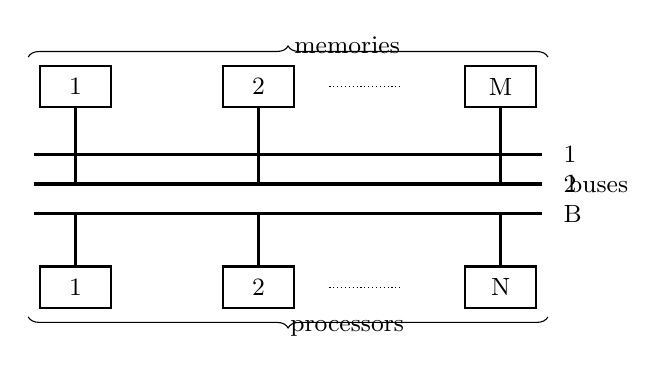
\begin{tikzpicture}[x=0.75cm,y=0.75cm]
  \draw[line width=0.9pt] (1,6.5) rectangle (2.2,7.2) node[midway]{\small 1};
  \draw[line width=0.9pt] (4.1,6.5) rectangle (5.3,7.2) node[midway]{\small 2};
  \draw[line width=0.9pt] (8.2,6.5) rectangle (9.4,7.2) node[midway]{\small M};
  \node at (6.2,7.55) {\small memories};
  \draw[decorate,decoration={brace,amplitude=4pt}] (0.8,7.35) -- (9.6,7.35);

  \draw[line width=1.1pt] (0.9,5.7) -- (9.5,5.7);
  \draw[line width=1.1pt] (0.9,5.2) -- (9.5,5.2);
  \draw[line width=1.1pt] (0.9,4.7) -- (9.5,4.7);
  \node[right] at (9.7,5.7) {\small 1};
  \node[right] at (9.7,5.2) {\small 2};
  \node[right] at (9.7,4.7) {\small B};
  \node at (10.45,5.2) {\small buses};

  \draw[line width=0.9pt] (1,3.1) rectangle (2.2,3.8) node[midway]{\small 1};
  \draw[line width=0.9pt] (4.1,3.1) rectangle (5.3,3.8) node[midway]{\small 2};
  \draw[line width=0.9pt] (8.2,3.1) rectangle (9.4,3.8) node[midway]{\small N};
  \node at (6.2,2.75) {\small processors};
  \draw[decorate,decoration={brace,mirror,amplitude=4pt}] (0.8,2.95) -- (9.6,2.95);

  \foreach \x in {1.6,4.7,8.8} {
    \draw[line width=0.9pt] (\x,6.5) -- (\x,5.2);
    \draw[line width=0.9pt] (\x,4.7) -- (\x,3.8);
  }
  \draw[densely dotted] (5.9,6.85) -- (7.1,6.85);
  \draw[densely dotted] (5.9,3.45) -- (7.1,3.45);
\end{tikzpicture}
\caption{Multiprocessor System Elements}
\end{figure}

\begin{enumerate}
\item A processor initiates a memory request at the start of a machine cycle
  and simultaneously suspends execution. Multiple requests for the same module
  are resolved by an arbitration mechanism. We'll assume that this mechanism
  tries to provide fair service via a cyclical scan of processors for requests,
  with the scan starting point being advanced on each new scan.
\item If a request is successful, the module is reserved for the processor;
  otherwise, the request is reissued at the start of the next cycle. From the
  set of up to $M$ successful requests, a second arbitration mechanism selects
  up to $B$ requests and reserves buses for these requests. We'll assume this is
  done in the same order in which modules were reserved. If a request is
  unsuccessful in obtaining a bus, the module is released and the request
  reissued at the start of the next cycle.
\item Next, for a successful request, the address and data (if the request is
  a store) are transmitted over the bus to memory; if the request is a fetch,
  data is returned over the bus at the end of the cycle.
\item When the bus cycle ends, processors whose requests were successfully
  completed are returned to execution, and the buses and modules reserved by
  these requests are released. Unsuccessful requests are reissued, together
  with new requests, at the start of the next cycle.
\end{enumerate}

Our objective is to determine how processor performance is affected by
contention for memory modules and buses.

This system, in various forms, has received a great deal of attention over
the years. When the number of buses is equal to the number of memories
($B = M$), the interconnection between processors and memories is equivalent to
a crossbar network, and performance is affected only by memory contention.
Most of the early analysis work focused on this problem; most recent work
encompasses systems with $B < M$ and considers both bus and memory contention.

\section{An Approximate Analytic Model}
\label{sec:mp-analytic-model}

The analytic model developed here is based on Mudge et al.\ [1984]; the
references in that paper provide a good starting point for surveying work in
this area. There are several measures of performance of interest; the one
considered first is system bandwidth, $BW$. This is the overall transfer rate
between processors and memory, in transfers per unit time. Since transfer time
is one cycle, overall bus utilization is (numerically, though not
dimensionally) equal to $BW$, and $BW$ is sometimes defined as the average
number of busy buses.

The miss ratio $p$ was defined as the probability that a processor issues a
(global) memory request in a given cycle. If we assume that the probability of
issuing a request in one cycle is the same as, and independent of, the
probability of issuing a request in any other cycle, then a processor's
execution interval corresponds to a sequence of Bernoulli trials. Execution
intervals therefore have a geometric distribution with mean
$x = (1-p)/p$ and variance $\sigma_x^2 = (1-p)/p^2$. We also assume that memory
requests are independently and uniformly distributed across memories.

Looking first at cycles with no reissued requests from the preceding cycle, the
probability that processor $i$ requests memory $j$ is $p/M$, and the
probability that none of the $N$ processors requests memory $j$ is
$(1 - p/M)^N$. Therefore the probability $q$ that there is at least one request
for memory $j$ is

\begin{equation}
q = 1 - (1 - p/M)^N
\label{eq:mp-q-p}
\end{equation}

Assuming request probabilities are identical and independent, the probability
$f_i$ that exactly $i$ of $M$ memories have requests is binomial:

\begin{equation}
f_i = \binom{M}{i} q^i (1-q)^{M-i}
\label{eq:mp-fi}
\end{equation}

The expected number of distinct memories requested in a cycle is $qM$. While up
to $qM$ requests may be presented to bus arbitration in a cycle, no more than
$B$ requests can be granted. The expected number of bus requests granted in a
cycle (equal numerically to bandwidth) is

\begin{equation}
BW = B\sum_{i=B}^{M} f_i + \sum_{i=1}^{B-1} i f_i
\label{eq:mp-bw}
\end{equation}

The bandwidth estimate from (\ref{eq:mp-q-p})--(\ref{eq:mp-bw}) applies only to
cycles in which no requests are reissued; in that case the average request rate
per processor is the miss rate $p$, and overall request rate is $Np$. In the
general case, considering all cycles, the per-processor request rate $r$ is
greater than $p$ (because it includes both initial and reissued requests). An
exact analysis is difficult; however, if we can estimate $r$, we can use it in
place of $p$ in (\ref{eq:mp-q-p}) to obtain an improved estimate of $BW$.

Now consider the processor inter-request interval between successful request
completions. Its mean overall length is $T$, and can be divided into three
parts: an execution interval of mean length $x = (1-p)/p$, a delay interval of
mean length $b$, and a one-cycle transfer time for the accepted request. The
single-processor request rate (counting blocked and accepted requests) is

\begin{figure}[ht]
\centering
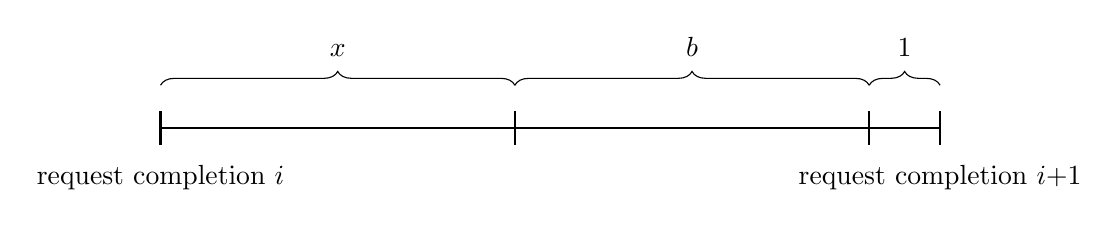
\begin{tikzpicture}[x=0.9cm,y=0.9cm]
  % Processor inter-request interval: execution x, blocked delay b, transfer 1.
  \draw[line width=0.9pt] (0,0) -- (11,0);
  \foreach \x in {0,5,10,11} {
    \draw[line width=0.9pt] (\x,0.24) -- (\x,-0.24);
  }
  \draw[decorate,decoration={brace,amplitude=5pt}] (0,0.6) -- (5,0.6)
    node[midway,above=7pt] {$x$};
  \draw[decorate,decoration={brace,amplitude=5pt}] (5,0.6) -- (10,0.6)
    node[midway,above=7pt] {$b$};
  \draw[decorate,decoration={brace,amplitude=5pt}] (10,0.6) -- (11,0.6)
    node[midway,above=7pt] {$1$};
  \node[below=10pt] at (0,0) {request completion $i$};
  \node[below=10pt] at (11,0) {request completion $i{+}1$};
\end{tikzpicture}
\caption{Processor Inter-Request Interval Timing}
\label{fig:ch5-inter-request-interval}
\end{figure}

\begin{equation}
r = (b+1)/T = (b+1)/(x+b+1)
\label{eq:mp-r}
\end{equation}

or

\begin{equation}
r = \left[1 + x/(b+1)\right]^{-1}
\label{eq:mp-r-alt}
\end{equation}

The per-processor request completion rate is $BW/N$, so $T = N/BW$, and
$b+1 = rT = Nr/BW$. Substituting in (\ref{eq:mp-r-alt}),

\begin{equation}
r = \left[1 + xBW/(Nr)\right]^{-1}
\label{eq:mp-r-fp}
\end{equation}

which defines $r$ as a fixed-point function of itself and can be solved
iteratively:

\begin{enumerate}
\item Use (\ref{eq:mp-q-p})--(\ref{eq:mp-bw}) to compute an initial bandwidth
  estimate $BW_1$. Define $r_1 = p$.
\item Compute an improved estimate of $r$ from
  \begin{equation}
  r_i = \left[1 + xBW_{i-1}/(Nr_{i-1})\right]^{-1}
  \label{eq:mp-ri}
  \end{equation}
\item Compute
  \begin{equation}
  q = 1 - (1-r_i/M)^N
  \label{eq:mp-q-r}
  \end{equation}
  and use (\ref{eq:mp-fi}) and (\ref{eq:mp-bw}) to compute a new estimate
  $BW_i$.
\item If $|BW_i - BW_{i-1}| < \epsilon$, where $\epsilon$ depends on desired
  accuracy, terminate; otherwise return to step 2.
\end{enumerate}

A C implementation with $\epsilon=0.005$ is shown in Figure~\ref{fig:ch5-bw-code}.

\begin{figure}[ht]
\centering
\begin{minipage}{0.86\textwidth}
\begin{verbatim}
real BW(real p, int B, int M, int N)
{
  real r = p, bw_prev = 0.0, bw = 0.0;
  while (1) {
    real q = 1.0 - pow(1.0 - r/M, N);
    bw = 0.0;
    for (int i = 1; i <= M; ++i) {
      real fi = comb(M,i) * pow(q,i) * pow(1-q, M-i);
      bw += (i < B) ? i*fi : B*fi;
    }
    if (fabs(bw - bw_prev) < 0.005) break;
    r = 1.0 / (1.0 + ((1-p)/p) * bw / (N*r));
    bw_prev = bw;
  }
  return bw;
}
\end{verbatim}
\end{minipage}
\caption{Bandwidth Computation Algorithm}
\label{fig:ch5-bw-code}
\end{figure}

Timing relationships and operational laws give other measures. Average
utilization of a single bus, memory module, and processor are respectively
$U_B = BW/B$, $U_M = BW/M$, and $U_P = xBW/N$. Average waiting time per request
is $b$, where from $T=N/BW$ and $x+1=1/p$:

\begin{equation}
b = (N/BW) - (1/p)
\label{eq:mp-b}
\end{equation}

Mean number of blocked requests per processor $L_b$ follows from Little's Law:

\begin{equation}
L_b = bBW/N
\label{eq:mp-lb}
\end{equation}

so

\begin{equation}
L_b = 1 - BW/(Np)
\label{eq:mp-lb-alt}
\end{equation}

For system throughput, if each task requires an average of $n$ execution
intervals, service time per task is $nx$. Throughput is $N[U_P/(nx)]$ tasks per
unit time. A normalized throughput $\eta$ with $nx=1$ is

\begin{equation}
\eta = N U_P = BW\left[(1/p)-1\right]
\label{eq:mp-eta}
\end{equation}

This bandwidth analysis is approximate, in part because
(\ref{eq:mp-q-p})--(\ref{eq:mp-fi}) assume independent memory request
probabilities. In the actual system, a blocked request for module $j$ is
reissued to $j$, so request probability for module $j$ in cycle $n$ is not
independent of cycle $n-1$. The next section develops a simulation model for
verification and evaluation of this assumption.

\section{Verifying the Analytic Model}
\label{sec:mp-verify}

The simulation model used for analytic verification depends on objective. Here
the objective is to verify that the analytic model adequately represents system
behavior, so the simulation model reflects system structure. A smpl model for
this purpose (called \texttt{bws1} in the book) is given in Figure 5.4.

\begin{figure}[ht]
\centering
\begin{minipage}{0.86\textwidth}
\begin{verbatim}
/* model bws1: synchronous multiprocessor */
init_model(p, N, M, B) {
  for (j=1; j<=M; j++) module[j] = facility("module", 1);
  bus = facility("bus", B);
  for (n=1; n<=N; n++) schedule(BEGIN_CYCLE, 0.0, n);
}

begin_cycle(n) {
  if (req[n] != 0) return;
  if (drand() < p) {
    req[n] = randint(1, M);
    schedule(REQ_MODULE, 0.0, n);
  } else {
    schedule(BEGIN_CYCLE, 1.0, n);
  }
}

req_module(n) {
  if (!busy(module[req[n]]) && !busy(bus)) {
    reserve(module[req[n]]); reserve(bus);
    schedule(END_CYCLE, 1.0, n);
  } else {
    schedule(REQ_MODULE, 1.0, n);   /* reissue */
  }
}

end_cycle(n) {
  release(module[req[n]]); release(bus);
  req[n] = 0; schedule(BEGIN_CYCLE, 0.0, n);
}
\end{verbatim}
\end{minipage}
\caption{Multiprocessor Simulation Model \texttt{bws1}}
\label{fig:ch5-bws1}
\end{figure}

In this model, memory modules and buses are smpl facilities, while processors
are represented as tokens. Global declarations define miss rate $p$, number of
processors $N$, memories $M$, and buses $B$ (named \texttt{nB} to avoid
conflict with \texttt{B()} in smpl), with facility descriptors
\texttt{module[]} and \texttt{bus}. \texttt{treg[n]} records next memory request
issue time for processor $n$, \texttt{req[n]} records requested module number,
and \texttt{tn} is the earliest request time. Initialization calls
\texttt{smpl()}, declares facilities, computes each initial access time, and
schedules the first event.

The continuation of the model appears in Figure~5.4 (continued): event 1
(\texttt{begin cycle()}) scans processors for requests at time \texttt{tn};
event 2 (\texttt{req module()}) requests memory and bus resources; and event 3
(\texttt{end cycle()}) releases resources and schedules follow-on work.

The geometric variate generation used in \texttt{next access()} is

\[
\left\lfloor \frac{\log(\texttt{ranf()})}{\log(1-p)} \right\rfloor
\]

which comes from the inverse distribution function of the geometric
distribution. Because of \texttt{floor()}, simulation times are integral cycle
counts.

This model is synchronous: the unit of time is the bus cycle, and events occur
at cycle boundaries. Since ``end of cycle $n$'' and ``beginning of cycle
$n+1$'' are the same simulation instant, event-list ordering alone is
insufficient; request starts and completions are batched explicitly.

At any simulation point, \texttt{treg[n]} is processor $n$'s next request issue
time, and \texttt{tn} is the earliest pending request time. \texttt{begin cycle}
schedules memory/bus request events for processors issuing at \texttt{tn},
advances the arbitration scan start point, and updates \texttt{tn} to the next
earliest issue time.

\texttt{req module()} checks whether both the target memory module and a bus are
free. If both are free, both are reserved and completion is scheduled one cycle
later. Otherwise, the request is blocked and reissued next cycle by incrementing
\texttt{treg[n]}. In this model, blocked requests are effectively reassigned
random destinations when reissued, matching the independence assumption of the
analytic model.

\texttt{end cycle()} releases reserved resources, computes the processor's next
access time, and when all completions in the current cycle are done, schedules
the next \texttt{begin cycle()} event. At run end, bus utilization is printed as
bandwidth; this numeric equivalence holds because bus service time is one cycle.

\paragraph{Output analysis.}
For verification runs, tighter confidence intervals are typically used than in
routine problem analysis so differences between analytic and simulation models
are less likely to be hidden by sampling variation. A sequential batch-means
procedure with continuous-time batches can be used here by sampling
\texttt{U(bus)} at fixed simulation intervals, resetting accumulators each
batch, and testing relative half-width against target accuracy.

\paragraph{Comparison strategy.}
Because this model has multiple parameters ($N$, $M$, $B$, and $p$), exhaustive
analytic-vs-simulation comparison is expensive. A practical approach is to
inspect response-shape plots (e.g., $BW$ vs.\ $B$ for fixed $N$, $M$, $p$) and
verify at:
\begin{itemize}
\item low-$B$ points (bus-limited region),
\item transition points where curvature changes,
\item high-$B$ points (memory-limited region).
\end{itemize}
If agreement is good at these structurally informative points, effort is then
shifted to other regions of parameter space.

\begin{figure}[ht]
\centering
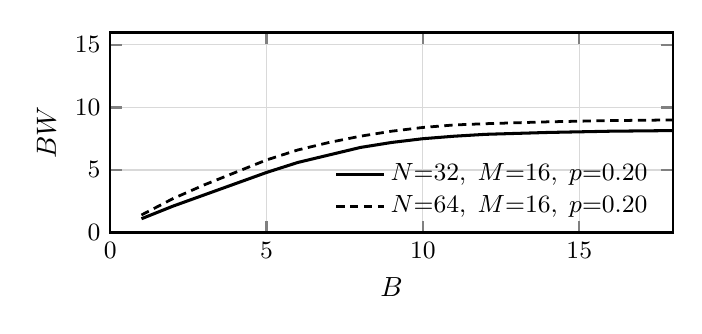
\begin{tikzpicture}
\begin{axis}[
  width=0.72\textwidth,
  height=0.34\textwidth,
  xmin=0,
  xmax=18,
  ymin=0,
  ymax=16,
  xlabel={$B$},
  ylabel={$BW$},
  axis line style={line width=0.9pt},
  tick style={line width=0.8pt},
  ticklabel style={font=\small},
  major grid style={draw=black!15},
  grid=major,
  legend style={font=\small,draw=none,fill=none,at={(0.98,0.02)},anchor=south east},
]
  % Response-shape sketch used to pick low/transition/high verification points.
  \addplot[line width=1.1pt] table[row sep=\\] {
    1 1.1\\
    2 2.1\\
    3 3.0\\
    4 3.9\\
    5 4.8\\
    6 5.6\\
    7 6.2\\
    8 6.8\\
    9 7.2\\
    10 7.5\\
    11 7.7\\
    12 7.85\\
    14 8.0\\
    16 8.1\\
    18 8.15\\
  };
  \addplot[densely dashed,line width=1.0pt] table[row sep=\\] {
    1 1.4\\
    2 2.7\\
    3 3.8\\
    4 4.8\\
    5 5.8\\
    6 6.6\\
    7 7.2\\
    8 7.7\\
    9 8.1\\
    10 8.4\\
    11 8.6\\
    12 8.7\\
    14 8.85\\
    16 8.95\\
    18 9.0\\
  };
  \addlegendentry{$N{=}32,\;M{=}16,\;p{=}0.20$}
  \addlegendentry{$N{=}64,\;M{=}16,\;p{=}0.20$}
\end{axis}
\end{tikzpicture}
\caption{Bandwidth Response Shape for Verification-Point Selection}
\label{fig:ch5-verification-shape}
\end{figure}

\section{A Synchronous Queueing Model}
\label{sec:mp-sync-queue}

The analytic model and \texttt{bws1} assume that a blocked request to module
$j$ may be reassigned randomly on reissue. To remove that assumption, a
queueing model is used in which module and bus requests are handled in
first-in, first-out order.

The queueing model structure (Figure~5.6) is still a closed queueing network.
Processors are represented by a delay server (no queueing at the processor
node). A request selects a memory module, queues for that module, then queues
for a bus, and transfer proceeds only when both resources are held. This
simultaneous resource possession is a common pattern in computer systems.

In this notation:
\begin{itemize}
\item memory modules are modeled as token-based resources (reserve/release),
\item buses are modeled as a multiserver queue.
\end{itemize}

\begin{figure}[ht]
\centering
\begin{tikzpicture}[node distance=1.2cm]
  \node[draw,circle,minimum size=0.9cm] (cpu1) {CPU};
  \node[draw,rectangle,minimum width=1.2cm,minimum height=0.8cm,right=2.2cm of cpu1] (mqueue) {M-queue};
  \node[draw,rectangle,minimum width=1.2cm,minimum height=0.8cm,right=1.8cm of mqueue] (mods) {M mods};
  \node[draw,rectangle,minimum width=1.2cm,minimum height=0.8cm,below=1.4cm of mods] (bqueue) {B-queue};
  \node[draw,rectangle,minimum width=1.2cm,minimum height=0.8cm,left=1.8cm of bqueue] (bus) {B buses};
  \node[draw,circle,minimum size=0.9cm,left=2.2cm of bus] (cpu2) {CPU};

  \draw[-{Stealth[length=3mm]},line width=0.9pt] (cpu1) -- node[above,sloped] {request} (mqueue);
  \draw[-{Stealth[length=3mm]},line width=0.9pt] (mqueue) -- (mods);
  \draw[-{Stealth[length=3mm]},line width=0.9pt] (mods) -- (bqueue);
  \draw[-{Stealth[length=3mm]},line width=0.9pt] (bqueue) -- (bus);
  \draw[-{Stealth[length=3mm]},line width=0.9pt] (bus) -- node[below,sloped] {completion} (cpu2);
  \draw[-{Stealth[length=3mm]},line width=0.9pt] (cpu2) to[bend left=20] node[left] {next cycle} (cpu1);
\end{tikzpicture}
\caption{Multiprocessor System Queueing Model Diagram}
\label{fig:ch5-queue-diagram}
\end{figure}

\paragraph{Simulation model \texttt{bws2}.}
A queueing-based model can be built by reusing parts of \texttt{bws1}
(declarations, initialization framework, and \texttt{begin cycle()}) and
replacing request/completion logic with separate module-queue and bus-queue
event routines (book Figure~5.7). In \texttt{main()}, switch dispatch is
adjusted accordingly, and \texttt{report()} can be used to obtain memory and bus
queue lengths in addition to utilizations.

Operationally, \texttt{bws2} remains synchronous. Processors with
\texttt{req[n] != 0} already have queued or active requests and are skipped in
\texttt{begin cycle()}. Module requests queue at module servers; admitted module
requests then queue at the bus server; transfer completion events mark requests
done and drive cycle-end release and scheduling logic.

\begin{figure}[ht]
\centering
\begin{minipage}{0.86\textwidth}
\begin{verbatim}
/* delta from bws1 to bws2 */
- req_module() reserves module and bus simultaneously
+ req_module() queues by module, then issues req_bus()

+ req_bus() {
+   if (busy(bus)) queue(bus); else reserve(bus);
+   schedule(END_CYCLE, 1.0, token);
+ }

- end_cycle() releases module/bus immediately
+ end_cycle() defers release until all cycle requests complete
+ and then triggers begin_cycle() for next machine cycle

+ report() now prints U(bus), U(module[j]), Q(module[j]), Q(bus)
\end{verbatim}
\end{minipage}
\caption{Changes to \texttt{bws1} for Memory and Bus Queueing}
\label{fig:ch5-bws2-delta}
\end{figure}

A key difference from \texttt{bws1} is that release operations are deferred
until all bus requests issued in the current cycle complete. Without this
deferral, resource release could trigger immediate dequeue/reschedule behavior
that invalidates cycle-level accounting.

\section{An Asynchronous Queueing Model}
\label{sec:mp-async-queue}

\texttt{bws1} and \texttt{bws2} are synchronous, fixed-cycle models. Queueing
network models are often used without strict synchronous constraints, so an
asynchronous variant is useful for comparison.

An asynchronous model (\texttt{bws3}) is obtained by simplifying \texttt{bws2}:
batching logic for cycle alignment is removed, event routines are compacted,
and processor execution intervals are generated from an exponential
distribution rather than geometric (since integer cycle counts are no longer
required).

\begin{figure}[ht]
\centering
\begin{minipage}{0.86\textwidth}
\begin{verbatim}
/* bws3 asynchronous model outline */
initialize modules[M], buses[B], processors[N]
for each processor n: schedule(ISSUE, expntl(1/p), n)

ISSUE(n):
  j = randint(1, M)
  if (module[j] and bus available) then
    reserve(module[j]); reserve(bus)
    schedule(COMPLETE, 1.0, n)
  else
    enqueue request (n,j)

COMPLETE(n):
  release resources for n
  schedule(ISSUE, expntl(1/p), n)
  dequeue waiting requests if resources become available
\end{verbatim}
\end{minipage}
\caption{Multiprocessor Simulation Model \texttt{bws3}}
\label{fig:ch5-bws3}
\end{figure}

\section{Model Results}
\label{sec:mp-results}

With the analytic model and simulation models (\texttt{bws1}, \texttt{bws2},
\texttt{bws3}), representative comparisons are shown in Table~\ref{tab:ch5-results}.

\begin{table}[ht]
\centering
\small
\begin{tabular}{rrrrrrrr}
\toprule
$N$ & $M$ & $B$ & $p$ & bwa & bws1 & bws2 & bws3 \\
\midrule
4 & 4 & 4 & 1.000 & 2.734 & 2.739 & 2.619 & 2.613 \\
4 & 4 & 2 & .500 & 1.583 & 1.668 & 1.664 & 1.665 \\
4 & 4 & 1 & .250 & .807 & .827 & .927 & .839 \\
4 & 2 & 1 & .125 & .481 & .487 & .737 & .484 \\
8 & 8 & 8 & 1.000 & 9.231 & 9.253 & 4.948 & 4.934 \\
8 & 8 & 4 & .500 & 3.273 & 3.379 & 3.334 & 3.352 \\
8 & 8 & 2 & .250 & 1.706 & 1.744 & 1.791 & 1.739 \\
8 & 4 & 2 & .250 & 1.690 & 1.711 & 1.718 & 1.709 \\
8 & 4 & 1 & .125 & .860 & .866 & .993 & .861 \\
16 & 16 & 16 & 1.000 & 10.303 & 10.305 & 9.614 & 9.586 \\
16 & 16 & 8 & .500 & 6.713 & 6.847 & 6.744 & 6.736 \\
16 & 16 & 4 & .250 & 3.553 & 3.598 & 3.601 & 3.596 \\
16 & 8 & 4 & .250 & 3.483 & 3.524 & 3.510 & 3.490 \\
16 & 8 & 2 & .125 & 1.794 & 1.794 & 1.810 & .877 \\
\bottomrule
\end{tabular}
\caption{Analytic and Simulation Model Results}
\label{tab:ch5-results}
\end{table}

In these comparisons, analytic and \texttt{bws1} bandwidths are generally close.
\texttt{bws2} and \texttt{bws3} are also close over most settings, with notable
differences for some single-bus configurations. The table supports two points:
(1) the analytic model is a useful approximation in much of the parameter
space, and (2) queueing semantics and synchrony assumptions can matter in edge
configurations.

\section{Extending the Multiprocessor System Model}
\label{sec:mp-extensions}

Natural extensions include:
\begin{itemize}
\item non-identical processors (different miss rates and execution
  distributions),
\item non-uniform/non-random memory addressing (including burst behavior),
\item variable transfer lengths (multi-cycle transfers),
\item different bus and memory service times.
\end{itemize}

All of these are straightforward to incorporate in the simulation framework
once processor/request state is explicitly represented.

\section{A CPU Modeling Project}
\label{sec:mp-cpu-project}

The chapter then introduces a project model of a pipelined CPU, intended as a
processor element that could sit inside the multiprocessor environment.
Principal elements are a four-stage instruction pipeline, a unified cache, an
instruction fetch buffer, and a data fetch buffer (Figure~5.9).

\begin{figure}[ht]
\centering
\begin{tikzpicture}[x=0.9cm,y=0.9cm]
  \node[draw,rectangle,minimum width=1.2cm,minimum height=0.8cm] (if) at (0,2.6) {Ifetch};
  \node[draw,rectangle,minimum width=1.2cm,minimum height=0.8cm] (pipeD) at (2.0,2.6) {D};
  \node[draw,rectangle,minimum width=1.2cm,minimum height=0.8cm] (pipeA) at (3.6,2.6) {A};
  \node[draw,rectangle,minimum width=1.2cm,minimum height=0.8cm] (pipeX) at (5.2,2.6) {X};
  \node[draw,rectangle,minimum width=1.2cm,minimum height=0.8cm] (pipeW) at (6.8,2.6) {W};
  \node[draw,rectangle,minimum width=2.0cm,minimum height=0.8cm] (cache) at (3.6,1.1) {Cache};
  \node[draw,rectangle,minimum width=1.2cm,minimum height=0.8cm] (df) at (6.8,1.1) {Dfetch};
  \draw[-{Stealth[length=3mm]},line width=0.9pt] (if) -- (pipeD);
  \draw[-{Stealth[length=3mm]},line width=0.9pt] (pipeD) -- (pipeA);
  \draw[-{Stealth[length=3mm]},line width=0.9pt] (pipeA) -- (pipeX);
  \draw[-{Stealth[length=3mm]},line width=0.9pt] (pipeX) -- (pipeW);
  \draw[-{Stealth[length=3mm]},line width=0.9pt] (pipeA) -- (cache);
  \draw[-{Stealth[length=3mm]},line width=0.9pt] (cache) -- (df);
  \draw[-{Stealth[length=3mm]},line width=0.9pt] (df) -- (pipeX);
\end{tikzpicture}
\caption{Major CPU Elements}
\label{fig:ch5-cpu-elements}
\end{figure}

Pipeline stages are fetch/decode (D), address generation (A), execute (X), and
write-back (W). At least one cycle is spent in each stage, so minimum
instruction latency is four cycles, while peak throughput is one instruction
per cycle due to overlap.

Branch and fetch/store behavior, cache arbitration, and multi-cycle execute
operations introduce holes and blocking effects in the completion stream, which
makes this a useful project for studying pipeline-control and memory-system
interaction under simulation.

Figure~5.10 in the original text illustrates representative pipeline sequences
and delay patterns for instruction classes:
\begin{itemize}
\item \textbf{FS}: load/store/non-taken branch instructions (issue cache request
  in first A cycle),
\item \textbf{BR}: taken branch instructions (issue target fetch in first A
  cycle),
\item \textbf{ALU}: arithmetic/logic instructions (may require multiple X
  cycles).
\end{itemize}

\begin{figure}[ht]
\centering
\begin{minipage}{0.86\textwidth}
\centering
\small
\begin{tabular}{l|cccccccc}
sequence & 1 & 2 & 3 & 4 & 5 & 6 & 7 & 8 \\ hline
(a) ALU  & D & A & X & W & D & A & X & W \\ 
(b) FS   & D & A & C & W & O & D & A & W \\ 
(c) BR   & D & A & B & O & O & D & A & W \\ 
(d) mix  & D & A & X & X & W & D & A & W \\ 
(e) mix  & D & A & B & O & D & A & X & W \\ 
\end{tabular}
\par\vspace{0.4em}
\footnotesize O = hole, C = cache arbitration delay, B = taken branch delay
\end{minipage}
\caption{Pipeline Sequence Examples}
\label{fig:ch5-pipeline-examples}
\end{figure}

In these sequences, \texttt{O} marks holes propagating through the pipeline and
\texttt{@} marks a delay cycle (a cycle in which no instruction completes).
Important effects shown in the examples:
\begin{itemize}
\item multi-X-cycle ALU instructions interlock following instructions;
\item FS requests can delay sequential instruction fetches and create holes;
\item taken branches can create multi-cycle holes due to target-fetch latency;
\item some holes are masked by other delays (e.g., long X-stage occupancy).
\end{itemize}

\paragraph{Workload description.}
Design evaluations for this project use the following instruction mix:

\begin{table}[ht]
\centering
\begin{tabular}{lr}
\toprule
Instruction type & Proportion \\
\midrule
BR  & 0.1437 \\
FS  & 0.4002 \\
ALU & 0.4561 \\
\midrule
Total & 1.0000 \\
\bottomrule
\end{tabular}
\caption{CPU Project Instruction Mix}
\label{tab:ch5-instr-mix}
\end{table}

FS instructions are approximately 49.5\% fetches, 17.5\% stores, and 33.0\%
non-taken branches. BR and FS instructions always have single-cycle X stages.
ALU instructions use a variable number of X cycles:

\begin{table}[ht]
\centering
\begin{tabular}{lr}
\toprule
ALU X cycles & Proportion of ALU instructions \\
\midrule
1  & 0.40 \\
2  & 0.40 \\
4  & 0.10 \\
8  & 0.07 \\
16 & 0.03 \\
\midrule
Total & 1.00 \\
\bottomrule
\end{tabular}
\caption{ALU Operation-Time Mix}
\label{tab:ch5-alu-mix}
\end{table}

Inter-branch headways (instructions between taken branches) are generated from
the distribution used earlier in Chapter 1. BR instructions terminate a
headway; other instructions in a headway are assigned independently as FS or
ALU according to the proportions above.

\paragraph{Building and validating the model.}
A compact smpl model is feasible (the original notes indicate under 100 lines
of C excluding debug instrumentation). A practical implementation strategy is to
compute stage transitions backward (W$\rightarrow$A) per cycle rather than
forward.

Validation in this project is primarily trace-based (in the absence of direct
analytic baselines for all behaviors). A useful cycle trace includes D/A/X/W
stage contents and key state such as Ifetch-buffer occupancy and sequential
fetch/branch flags.

\paragraph{Pipeline design analyses.}
Primary performance metric: mean instruction execution time per instruction,
$I$ cycles/instruction. If cycle time is $C$ microseconds, throughput in MIPS is
$(IC)^{-1}$. Also collect mean X-stage cycles per instruction, $E$; branch/Ifetch
delay contribution is then $D = I - E$.

The base case is Ifetch-buffer capacity of one instruction. Alternatives to
evaluate relative to this baseline:
\begin{enumerate}
\item increase Ifetch-buffer capacity to 2, 3, or 4 instructions;
\item widen cache$\rightarrow$Ifetch path so sequential/target fetch can return two
  instructions per cache access (with and without enforced branch-target
  alignment);
\item delayed-branch architecture variant where the sequential instruction
  following a branch always executes (assume useful work 70\%, NOP 30\%);
\item repeat evaluations assuming multi-cycle ALU execution times are reduced by
  50\% in a future implementation.
\end{enumerate}

% OCR draft from PDF pages 160-162 (book pages 182-184 in scan).
\chapter{An Ethernet Model}
\label{chap:ethernet-model}

\section{Introduction}
\label{sec:ether-introduction}

This chapter presents a macroscopic simulation model of an Ethernet local area
network. The model (called \texttt{ether}) is used to study how load
characteristics, such as message rates and message-length distributions, affect
performance, and to experiment with protocol and load-adaptive algorithms.

Analytic and measurement results from the literature are used to verify and
validate \texttt{ether}. The Ethernet model introduces new timing and
coordination issues relative to the synchronous multiprocessor model of the
preceding chapter. In particular, occurrence of an event may be recognized at
different instants at different stations because of propagation delay. Other
topics include efficient representation of many request sources and variate
generation from truncated distributions.

\section{The Ethernet Network}
\label{sec:ether-network}

The modeled network comprises $N$ stations connected by a coaxial channel.
Stations attach through cable taps and transceivers, with transceiver cables to
station controllers.

\begin{figure}[ht]
\centering
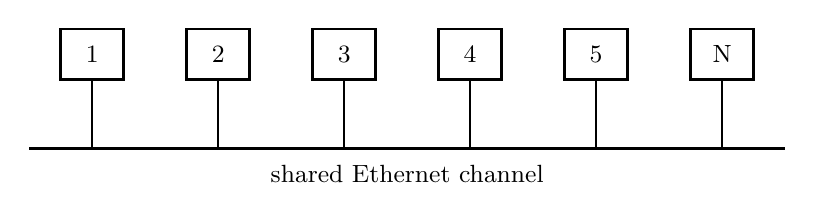
\begin{tikzpicture}[x=0.8cm,y=0.8cm]
  \draw[line width=1.1pt] (0,2.5) -- (12,2.5);
  \foreach \x/\n in {1/1,3/2,5/3,7/4,9/5,11/N} {
    \draw[line width=0.9pt] (\x,2.5) -- (\x,3.6);
    \draw[line width=0.9pt] (\x-0.5,3.6) rectangle (\x+0.5,4.4);
    \node at (\x,4.0) {\small \n};
  }
  \node at (6,2.1) {\small shared Ethernet channel};
\end{tikzpicture}
\caption{A Simple Ethernet Network}
\label{fig:ether-simple-network}
\end{figure}

Ethernet communication behavior is implemented by controller hardware (and
microcode) together with station software; exact partitioning depends on the
implementation. In general deployments, stations may be computers,
workstations, file servers, printers, and other devices. For this model,
stations are assumed identical.

Ethernet supports up to 1024 stations and a total cable length of 2.5 km in a
non-rooted tree interconnection, with repeaters for long segments. Data is
transmitted serially at 10 Mbps. Ethernet is specified in detail in
[DEC et al 1982], with a close ANSI/IEEE counterpart in 802.3.

\subsection*{Data format}

Data is transmitted in frames containing preamble, header, data, and CRC.

\begin{figure}[ht]
\centering
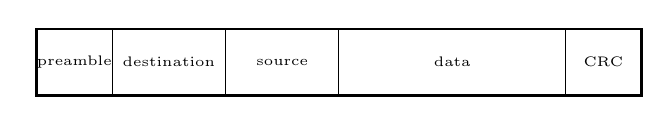
\begin{tikzpicture}[x=0.12cm,y=0.7cm]
  \draw[line width=1pt] (0,0) rectangle (64,1.2);
  \draw (8,0) -- (8,1.2); \draw (20,0) -- (20,1.2);
  \draw (32,0) -- (32,1.2); \draw (56,0) -- (56,1.2);
  \node at (4,0.6) {\tiny preamble};
  \node at (14,0.6) {\tiny destination};
  \node at (26,0.6) {\tiny source};
  \node at (44,0.6) {\tiny data};
  \node at (60,0.6) {\tiny CRC};
\end{tikzpicture}
\caption{Ethernet Frame Format}
\label{fig:ether-frame-format}
\end{figure}

The data field length is 46--1500 bytes. Shorter messages are padded to the
minimum. Header fields carry destination/source addresses and data length
(excluding padding). The CRC supports error checking at the receiver.

Before frame data, a station sends a 64-bit synchronization preamble. With
$L$ as data-field length in bytes, nominal frame transmission time is:

\begin{equation}
t_f = 20.8 + 0.8L \quad \text{microseconds}
\label{eq:ether-tf}
\end{equation}

Hence the minimum frame time (at $L=46$) is 57.6 microseconds.

\subsection*{Channel access protocol}

Ethernet uses Carrier Sense Multiple Access with Collision Detection
(CSMA/CD). A station with data to send senses the channel; if idle, it starts
transmission. There is an inter-frame gap between sensing idle and transmission
start to ensure receiving stations complete end-of-frame processing before a
new transmission begins.

During transmission, the sender continues sensing the channel. If another
station starts in the collision window, a collision occurs. A station that
detects collision aborts frame data transmission, sends a jam sequence so all
stations recognize the collision, and schedules a retransmission after a random
backoff delay.

\begin{figure}[ht]
\centering
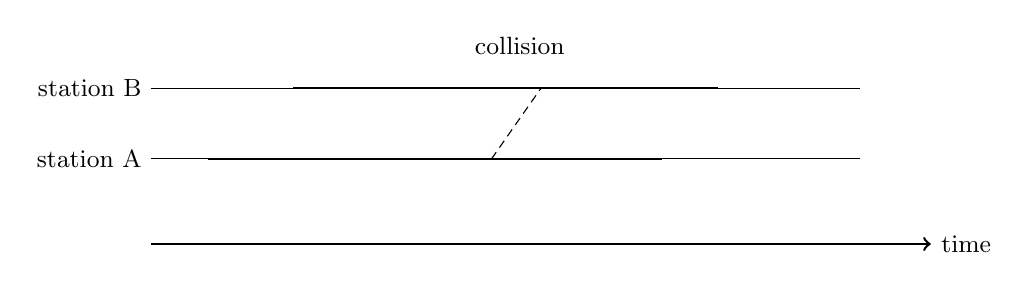
\begin{tikzpicture}[x=0.9cm,y=0.9cm]
  \draw[->,line width=0.9pt] (0,0) -- (11,0) node[right]{\small time};
  \draw (0,1.2) node[left]{\small station A} -- (10,1.2);
  \draw (0,2.2) node[left]{\small station B} -- (10,2.2);
  \draw[line width=1pt] (0.8,1.2) -- (4.8,1.2);
  \draw[line width=1pt] (2.0,2.2) -- (5.5,2.2);
  \draw[densely dashed] (4.8,1.2) -- (5.5,2.2);
  \node at (5.2,2.8) {\small collision};
  \draw[line width=0.9pt] (5.5,2.2) -- (8.0,2.2);
  \draw[line width=0.9pt] (4.8,1.2) -- (7.2,1.2);
\end{tikzpicture}
\caption{Colliding Transmissions in Ethernet}
\label{fig:ether-collision-timing}
\end{figure}

Let $\tau$ be end-to-end propagation delay and $T_{\text{jam}}$ jam time. In the
worst case, colliding stations each transmit for approximately
$2\tau + T_{\text{jam}}$ before backing off. A station that has transmitted for
$2\tau$ without collision has effectively acquired the channel for successful
completion.

With Ethernet's maximum round-trip propagation of 45 bit-times,
$\tau_{\max}=22.5\,\mu s$. With maximum jam length 48 bit-times,
$T_{\text{jam}}=4.8\,\mu s$. Thus a collision fragment can be up to 498 bit-times
($49.8\,\mu s$), which motivates the minimum valid frame size (excluding
preamble) of 64 bytes.

\paragraph{Slot time.}
The slot time $T_{\text{slot}}$ is specified as 512 bit-times ($51.2\,\mu s$).
It is the backoff rescheduling quantum. It must exceed both acquisition and
collision-fragment timing requirements while remaining small enough to avoid
unnecessary latency inflation.

\paragraph{Backoff algorithm.}
Ethernet uses truncated binary exponential backoff:
\begin{enumerate}
\item increment retransmission attempt count $n$;
\item if $n>16$, report transmission error;
\item set $k=\min(n,10)$;
\item draw random integer $r \in [0,2^k-1]$;
\item backoff delay is $r$ slot-times.
\end{enumerate}
So attempt 1 backs off 0--1 slots; attempt 2, 0--3; \ldots; attempts 10--16,
0--1023 slots.

\section{Performance Parameters and Measures}
\label{sec:ether-metrics}

The model focuses on throughput and mean frame delay as functions of offered
load, station count, inter-transmission intervals, and mean frame length.

Let $S$ denote network throughput in the common utilization-based form (fraction
of channel use carrying successful frame data). Let $T_d$ be mean frame delay
from first transmission attempt to successful completion, including queueing,
collision recovery, backoff, and transfer time.

With $T_f$ as mean no-contention frame transmission time, normalized delay is:

\begin{equation}
D = T_d / T_f
\label{eq:ether-D}
\end{equation}

For closed-system interpretation with $N$ identical stations and mean
inter-transmission interval $T_i$ (post-completion to next attempt):

\begin{equation}
G = \frac{N T_f}{T_i + T_f}
\label{eq:ether-G-closed}
\end{equation}

For open-system interpretation with external arrival rate $\lambda$:

\begin{equation}
G = \lambda T_f
\label{eq:ether-G-open}
\end{equation}

A key Ethernet parameter is

\begin{equation}
\alpha = \tau/T_f
\label{eq:ether-alpha}
\end{equation}

For fixed offered load, larger $\alpha$ (shorter frames relative to
propagation) implies more collision overhead and lower throughput.

\section{Lam's Model}
\label{sec:ether-lam}

Lam [1980] gives an analytic upper bound on CSMA/CD throughput:

\begin{equation}
S_{\max} = \left[1 + \alpha(1 + 2e)\right]^{-1}
\label{eq:ether-smax}
\end{equation}

\begin{figure}[ht]
\centering
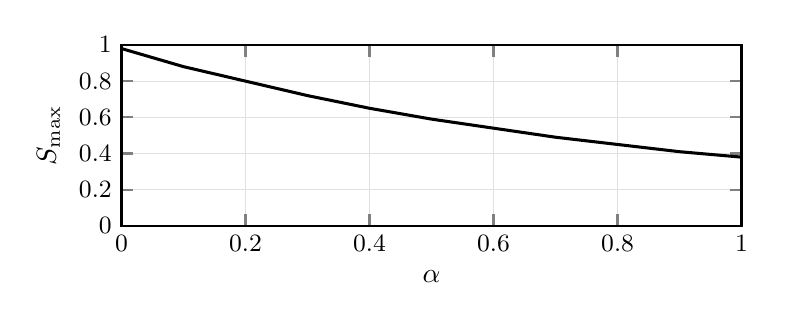
\begin{tikzpicture}
\begin{axis}[
  width=0.78\textwidth,height=0.32\textwidth,
  xmin=0,xmax=1,ymin=0,ymax=1,
  xlabel={$\alpha$},ylabel={$S_{\max}$},
  axis line style={line width=0.9pt},tick style={line width=0.8pt},
  ticklabel style={font=\small},grid=major,major grid style={draw=black!12}
]
\addplot[line width=1.1pt] table[row sep=\\]{
0.00 0.98\\ 0.05 0.93\\ 0.10 0.88\\ 0.20 0.80\\ 0.30 0.72\\
0.40 0.65\\ 0.50 0.59\\ 0.60 0.54\\ 0.70 0.49\\ 0.80 0.45\\ 0.90 0.41\\ 1.00 0.38\\
};
\end{axis}
\end{tikzpicture}
\caption{Maximum Network Throughput as a Function of $\alpha$}
\label{fig:ether-smax}
\end{figure}

Lam also provides a closed-form expression for $T_d$ in terms of
$\tau,\lambda,T_f$, moments of frame-time distribution, and Laplace transform
$B^*(\cdot)$. For constant frame lengths:
\begin{equation}
T_{f2}=T_f^2
\label{eq:ether-tf2-const}
\end{equation}
\begin{equation}
B^*(\lambda)=e^{-\lambda T_f}
\label{eq:ether-bstar-const}
\end{equation}
For exponentially distributed frame lengths:
\begin{equation}
T_{f2}=2T_f^2
\label{eq:ether-tf2-exp}
\end{equation}
\begin{equation}
B^*(\lambda)=\frac{1}{1+\lambda T_f}
\label{eq:ether-bstar-exp}
\end{equation}

The chapter includes C code for computing Lam delay (Figure 6.5).

\begin{figure}[ht]
\centering
\begin{minipage}{0.86\textwidth}
\begin{verbatim}
real lam_delay(real alpha, real rho)
{
  /* Lam approximation for non-persistent CSMA/CD */
  real a2 = alpha * alpha;
  real num = 1.0 + alpha * (1.0 + 4.5*alpha);
  real den = 2.0 * (1.0 - rho);
  real coll = rho * (1.0 + 2.0*alpha + a2) / (1.0 - rho);
  return num/den + coll;
}
\end{verbatim}
\end{minipage}
\caption{Function to Compute Lam's Mean Frame Delay}
\label{fig:ether-lam-c}
\end{figure}

\section{The \texttt{ether} Simulation Model}
\label{sec:ether-model}

In \texttt{ether}, the network is represented as a closed system with one shared
server (channel) and a station pool as request sources. Channel state is tracked
by simple variables; stations are modeled as tokens generating requests at
random (exponentially distributed inter-request intervals), contending for
channel access, and scheduling the next request after successful completion.

A central modeling issue is propagation delay. For a macroscopic model with
indistinguishable stations, timing is represented probabilistically rather than
by exact geometric station coordinates.

Assume $N$ stations equally spaced; let $d=|i-j|$ be unit distance between the
most recent channel owner $i$ and requesting station $j$. Then:

\begin{equation}
\Pr[x=d]=\frac{2(N-d)}{N(N-1)}, \quad 1\le d \le N-1
\label{eq:ether-dist-pmf}
\end{equation}

\begin{equation}
\Pr[x \le d]=\sum_{k=1}^{d}\frac{2(N-k)}{N(N-1)}
\label{eq:ether-dist-cdf-sum}
\end{equation}

\begin{equation}
\Pr[x \le d]=\frac{2Nd-d(d+1)}{N(N-1)}
\label{eq:ether-dist-cdf}
\end{equation}

For large $N$ this is approximated by:
\begin{equation}
\Pr[x \le d] \approx 1-\left(1-\frac{d}{N}\right)^2
\label{eq:ether-dist-cdf-approx}
\end{equation}

For convenience, the inter-station distance distribution is treated as
continuous, giving the random-distance generator

\begin{equation}
d = N\left[1-r^{1/2}\right]
\label{eq:ether-rand-distance}
\end{equation}

where $r$ is uniform on $[0,1]$. Since propagation delay per unit distance is
approximately $\tau/N$ for large $N$, a sample propagation delay between the
requesting station and the station last reserving/releasing the channel is

\begin{equation}
d_t = \tau\left[1-r^{1/2}\right]
\label{eq:ether-rand-delay}
\end{equation}

\subsection*{Modeling request arrivals}

With identical stations and exponential inactive intervals, request arrivals can
be modeled with a single next-arrival event instead of one outstanding event per
station.

At a given instant, let $n$ be the number of inactive stations and $T_i$ the
mean inactive interval per station. For one station, remaining inactive time
$y$ has

\begin{equation}
\Pr[y<t] = 1-e^{-t/T_i}
\label{eq:ether-y-cdf}
\end{equation}

If $x=\min(y_1,\ldots,y_n)$, then

\begin{equation}
\Pr[x<t] = 1-\{1-\Pr[y<t]\}^{n}
\label{eq:ether-min-cdf}
\end{equation}

which simplifies to

\begin{equation}
\Pr[x<t] = 1-e^{-nt/T_i}
\label{eq:ether-next-arrival-cdf}
\end{equation}

So the time to next request from the inactive pool is exponential with mean
$T_i/n$. This supports an efficient algorithm with exactly one queued
arrival event regardless of $N$.

\subsection*{Event routines}

The model uses six events (Figure~6.6): transmission arrival, deference check,
transmission start, transmission end, backoff initialization, and channel
deassert/release.

\begin{figure}[ht]
\centering
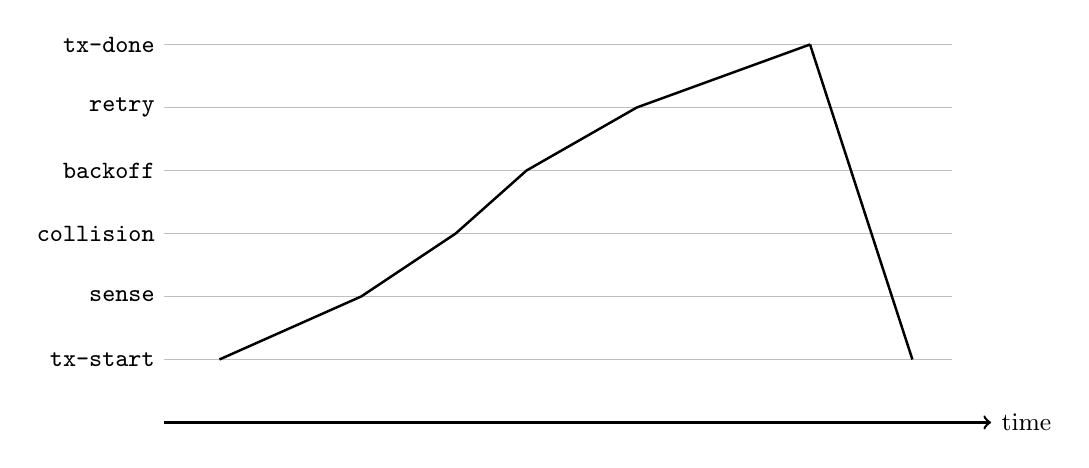
\begin{tikzpicture}[x=1cm,y=0.8cm]
  \draw[->,line width=0.9pt] (0,0) -- (10.5,0) node[right]{\small time};
  \node[left] at (0,1) {\small \texttt{tx-start}};
  \node[left] at (0,2) {\small \texttt{sense}};
  \node[left] at (0,3) {\small \texttt{collision}};
  \node[left] at (0,4) {\small \texttt{backoff}};
  \node[left] at (0,5) {\small \texttt{retry}};
  \node[left] at (0,6) {\small \texttt{tx-done}};
  \foreach \y in {1,2,3,4,5,6} {\draw[black!25] (0,\y) -- (10,\y);}
  \draw[line width=0.9pt] (0.7,1) -- (2.5,2) -- (3.7,3) -- (4.6,4) -- (6.0,5) -- (8.2,6);
  \draw[line width=0.9pt] (8.2,6) -- (9.5,1);
\end{tikzpicture}
\caption{\texttt{ether} Simulation Model Events}
\label{fig:ether-events}
\end{figure}

\textbf{TransmitFrame:} initializes attempt/backoff counters, records request
arrival time for delay measurement, schedules deference processing, decrements
inactive-station count, and schedules the next arrival using the single-event
arrival process.

\textbf{Defer:} evaluates whether a requester senses channel busy or idle,
accounting for propagation delay and inter-frame gap timing. Channel state is
tracked by status variable plus timestamps for last busy/idle transitions.

\begin{figure}[ht]
\centering
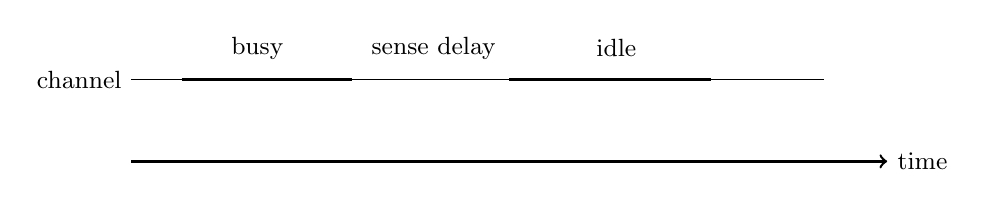
\begin{tikzpicture}[x=0.8cm,y=0.8cm]
  \draw[->,line width=0.9pt] (0,0) -- (12,0) node[right]{\small time};
  \draw (0,1.3) node[left]{\small channel} -- (11,1.3);
  \draw[line width=0.9pt] (0.8,1.3) -- (3.5,1.3);
  \draw[densely dotted] (3.5,1.3) -- (6.0,1.3);
  \draw[line width=0.9pt] (6.0,1.3) -- (9.2,1.3);
  \node at (2.0,1.8) {\small busy};
  \node at (4.8,1.8) {\small sense delay};
  \node at (7.7,1.8) {\small idle};
\end{tikzpicture}
\caption{Channel State Sensing Timing}
\label{fig:ether-sensing-timing}
\end{figure}

If busy is sensed, request is placed on defer-wait list. If idle is sensed,
remaining deference time is computed and StartTransmit is scheduled.

\begin{figure}[ht]
\centering
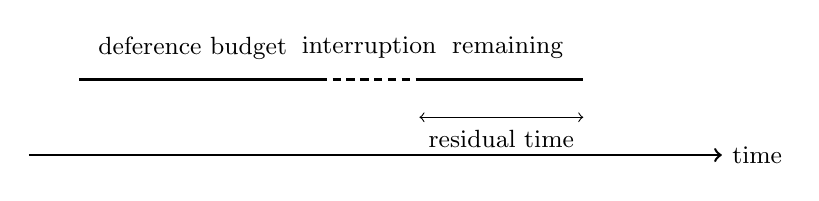
\begin{tikzpicture}[x=0.8cm,y=0.8cm]
  \draw[->,line width=0.9pt] (0,0) -- (11,0) node[right]{\small time};
  \draw[line width=0.9pt] (0.8,1.2) -- (4.6,1.2);
  \draw[densely dashed,line width=0.8pt] (4.6,1.2) -- (6.2,1.2);
  \draw[line width=0.9pt] (6.2,1.2) -- (8.8,1.2);
  \node at (2.6,1.7) {\small deference budget};
  \node at (5.4,1.7) {\small interruption};
  \node at (7.6,1.7) {\small remaining};
  \draw[<->] (6.2,0.6) -- (8.8,0.6);
  \node at (7.5,0.25) {\small residual time};
\end{tikzpicture}
\caption{Remaining Deference Time Computation}
\label{fig:ether-defer-time}
\end{figure}

\textbf{StartTransmit:} if channel is idle, reserves channel and schedules
successful completion candidate. If busy, collision is inferred: colliders are
scheduled into backoff processing and current successful-completion event may be
canceled for first detected collision in the window.

\textbf{EndTransmit:} accumulates delay statistics for successful frame,
schedules channel deassert/release, increments inactive count, and reschedules
single next-arrival event.

\textbf{InitBackoff:} applies truncated binary exponential backoff. Requests
with attempts $>16$ are dropped and source is returned to inactive pool;
otherwise requester either re-enters deference immediately (0 slots) or is
scheduled after nonzero backoff.

\textbf{Deassert:} transitions channel to idle and reactivates deferred
requests by scheduling StartTransmit after propagation plus inter-frame gap.

\section{The \texttt{ether} Simulation Program}
\label{sec:ether-program}

Figure~6.9 contains a smpl implementation of \texttt{ether}. Parameters are
defined via macros and globals (e.g., propagation delay, inter-frame gap, slot
time, jam time, station count, offered load, and $\alpha$), and event routines
directly implement the six-event logic above.

\begin{figure}[ht]
\centering
\begin{minipage}{0.86\textwidth}
\begin{verbatim}
/* ether: simplified event-driven CSMA/CD model */
main() {
  init_model();
  while (time() < TMAX) {
    cause(&ev, &src);
    switch(ev) {
      case GEN:   gen_frame(src); break;
      case SENSE: sense_channel(src); break;
      case START: start_tx(src); break;
      case COLL:  collision(src); break;
      case END:   end_tx(src); break;
      case RETRY: retry_tx(src); break;
    }
  }
  report_stats();
}
\end{verbatim}
\end{minipage}
\caption{The \texttt{ether} Simulation Program}
\label{fig:ether-program}
\end{figure}

The program estimates throughput $S$ and normalized delay $D$ as functions of
$\alpha$ and $G$. During initialization, mean frame transmission time $T_f$ and
mean inactive time $T_i$ are computed from
(\ref{eq:ether-G-closed}) and (\ref{eq:ether-alpha}). Requests are represented
with descriptor records linked through available/defer lists.

\section{\texttt{ether} Verification and Validation}
\label{sec:ether-verify-validate}

The model is checked by comparison to both Lam-model results and measured
Ethernet data.

\paragraph{Comparison with Lam-model results.}
Runs were made across $\alpha$ values (roughly 0.01--0.25) and offered loads
$G$ increasing toward saturation. For each fixed $\alpha$, throughput and delay
curves were generated and $S_{\max}$ estimated near the high-delay knee.

For smaller $\alpha$ values, simulated $S_{\max}$ tracks Lam's bound closely.
At larger $\alpha$, differences grow, largely due to model-assumption mismatch
(collision interval treatment and open-vs-closed modeling effects near
saturation).

\begin{figure}[ht]
\centering
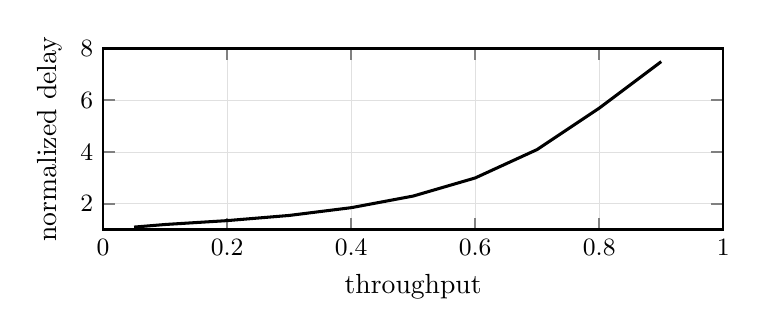
\begin{tikzpicture}
\begin{axis}[
  width=0.78\textwidth,height=0.32\textwidth,
  xmin=0,xmax=1,ymin=1,ymax=8,
  xlabel={throughput},ylabel={normalized delay},
  axis line style={line width=0.9pt},tick style={line width=0.8pt},
  ticklabel style={font=\small},grid=major,major grid style={draw=black!12}
]
\addplot[line width=1.1pt] table[row sep=\\]{
0.05 1.1\\ 0.10 1.2\\ 0.20 1.35\\ 0.30 1.55\\ 0.40 1.85\\
0.50 2.3\\ 0.60 3.0\\ 0.70 4.1\\ 0.80 5.7\\ 0.90 7.5\\
};
\end{axis}
\end{tikzpicture}
\caption{Normalized Delay versus Throughput at $\alpha=0.05$}
\label{fig:ether-delay-vs-throughput}
\end{figure}

\paragraph{Comparison with measurement data.}
To align with reported measurements (Gonsalves), simulation settings are
adjusted (notably smaller $N$, different $\tau$, constant frame lengths, and
uniform inactive intervals). Throughput definitions are also aligned: measured
throughput may be based on data bytes only, while simulation throughput is often
based on total frame time.

If $\alpha'$ is based on frame length excluding preamble and $\alpha$ includes
preamble, the relationship used is

\begin{equation}
\alpha = \alpha' \left(1 + \frac{8}{L'}\right)
\label{eq:ether-alpha-prime}
\end{equation}

Representative throughput comparison:

\begin{table}[ht]
\centering
\begin{tabular}{lccc}
\toprule
Frame bytes & $\alpha'$ & Gonsalves $S'$ & \texttt{ether} $S'$ \\
\midrule
64   & .280 & .26 & .28 \\
200  & .092 & .60 & .57 \\
512  & .026 & .72 & .72 \\
1500 & .012 & .85 & .83 \\
\bottomrule
\end{tabular}
\caption{Measurement and Simulation Throughput Results}
\label{tab:ether-measurement-compare}
\end{table}

\section{Applications and Extensions}
\label{sec:ether-extensions}

\texttt{ether} supports experimentation with protocol and collision-recovery
variants. Common extensions include:
\begin{itemize}
\item alternate backoff schemes,
\item load-adaptive access controls,
\item priority-aware or mixed-traffic policies,
\item variable frame-length distributions.
\end{itemize}

Variable frame lengths are important for realism (short control frames mixed
with long data frames). One practical variant is a truncated exponential frame
time model honoring Ethernet minimum/maximum frame constraints.

\subsection*{Generating variates from a truncated exponential}

For exponential variable $t$ with parameter $u$:

\begin{equation}
E[t] = \int_0^\infty t\,u e^{-ut}\,dt
\label{eq:ether-trunc-mean}
\end{equation}

Splitting at $t_{\min}$:

\begin{equation}
E[t] = \int_0^{t_{\min}} t\,u e^{-ut}\,dt + \int_{t_{\min}}^\infty t\,u e^{-ut}\,dt
\label{eq:ether-trunc-split}
\end{equation}

Replacing samples below $t_{\min}$ by $t_{\min}$ contributes

\begin{equation}
w = t_{\min}\Pr[t < t_{\min}] = t_{\min}\left(1-e^{-u t_{\min}}\right)
\label{eq:ether-trunc-w}
\end{equation}

and yields a target mean form

\begin{equation}
T_f = t_{\min}\left(1-e^{-u t_{\min}}\right) + \int_{t_{\min}}^\infty t\,u e^{-ut}\,dt
\label{eq:ether-trunc-tf}
\end{equation}

which simplifies to

\begin{equation}
T_f = t_{\min} + u^{-1}e^{-u t_{\min}}
\label{eq:ether-trunc-simplified}
\end{equation}

Since $u$ is implicit, Newton iteration is used in practice (book Eq.\ 6.25).

\section{Summary}
\label{sec:ether-summary}

This chapter develops a compact macroscopic Ethernet model using analytic
submodels to reduce detail while preserving key contention behavior. It is not
a full hybrid model in the strict sense, but it demonstrates how probabilistic
substructure can simplify event simulation and still support verification and
validation against analytic bounds and measured data.

\section{A Token Ring Modeling Project}
\label{sec:token-ring-project}

The project asks for a token-ring simulation model to study effects of ring
configuration and workload parameters.

\begin{figure}[ht]
\centering
\begin{tikzpicture}[x=1cm,y=1cm]
  \draw[line width=1pt] (0,0) circle (2.4);
  \foreach \a/\n in {90/1,18/2,-54/3,-126/4,162/N} {
    \node[draw,rectangle,minimum width=0.9cm,minimum height=0.6cm] at (\a:2.4) {\small \n};
  }
  \draw[-{Stealth[length=3mm]},line width=0.9pt] (30:2.4) arc[start angle=30,end angle=-20,radius=2.4];
  \node at (0,-3.0) {\small token circulates in ring direction};
\end{tikzpicture}
\caption{A Token Ring Network}
\label{fig:token-ring-network}
\end{figure}

Token and frame formats:

\begin{figure}[ht]
\centering
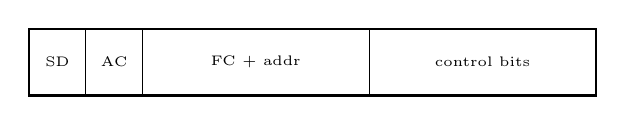
\begin{tikzpicture}[x=0.18cm,y=0.7cm]
  \draw[line width=1pt] (0,0) rectangle (40,1.2);
  \draw (4,0)--(4,1.2); \draw (8,0)--(8,1.2); \draw (24,0)--(24,1.2);
  \node at (2,0.6) {\tiny SD};
  \node at (6,0.6) {\tiny AC};
  \node at (16,0.6) {\tiny FC + addr};
  \node at (32,0.6) {\tiny control bits};
\end{tikzpicture}
\caption{Token Format}
\label{fig:token-format}
\end{figure}

\begin{figure}[ht]
\centering
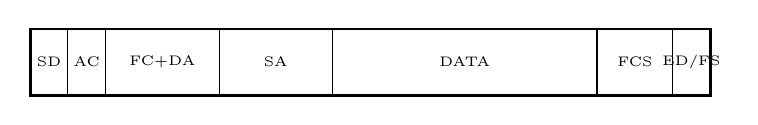
\begin{tikzpicture}[x=0.12cm,y=0.7cm]
  \draw[line width=1pt] (0,0) rectangle (72,1.2);
  \foreach \x in {4,8,20,32,60,68} {\draw (\x,0)--(\x,1.2);} 
  \node at (2,0.6) {\tiny SD};
  \node at (6,0.6) {\tiny AC};
  \node at (14,0.6) {\tiny FC+DA};
  \node at (26,0.6) {\tiny SA};
  \node at (46,0.6) {\tiny DATA};
  \node at (64,0.6) {\tiny FCS};
  \node at (70,0.6) {\tiny ED/FS};
\end{tikzpicture}
\caption{Token Ring Frame Format}
\label{fig:token-frame-format}
\end{figure}

Core network parameters:
\begin{equation}
\tau = 5K + \frac{BN}{R}
\label{eq:token-latency}
\end{equation}
\begin{equation}
T_f = \frac{L}{R}
\label{eq:token-tf}
\end{equation}
\begin{equation}
\alpha = \frac{\tau}{T_f}
\label{eq:token-alpha}
\end{equation}
\begin{equation}
S = N\lambda T_f
\label{eq:token-throughput}
\end{equation}

The chapter also provides a closed-form mean-delay expression (Eq.\ 6.31) for a
symmetric token-ring case under simplifying assumptions (Poisson arrivals,
constant frame length, uniform station spacing, and $\alpha<1$), and then asks
for simulation-based verification and exploration.

Project tasks include:
\begin{enumerate}
\item verify model behavior against Eq.\ 6.31 for baseline parameters;
\item study ring-latency impact by changing cable length and station overhead;
\item study asymmetric-arrival effects (small high-load subset of stations);
\item extend to a file-server ring workload and estimate read response-time
  components (network vs disk).
\end{enumerate}

% OCR draft from PDF pages 220-234 (book chapter 7).
\chapter{A Simulation Environment}
\label{chap:simulation-environment}

\section{Introduction}
\label{sec:simenv-intro}

This chapter presents a user-level view of the SMPL simulation environment.
SMPL includes:
\begin{itemize}
\item the \texttt{smpl} subsystem from Chapter 2,
\item debugging/analysis/reporting tools,
\item an interactive run-time interface called \texttt{mtr}.
\end{itemize}

In the implementation described (SMPL/PC), \texttt{mtr} acts as the interactive
front-end between user, simulation model, and support modules.

\begin{figure}[ht]
\centering
\fbox{\parbox[c][5cm][c]{0.86\textwidth}{\centering Figure 7.1 placeholder (SMPL simulation environment)}}
\caption{The SMPL Simulation Environment}
\label{fig:smpl-environment}
\end{figure}

Main optional modules:
\begin{itemize}
\item \textbf{dump}: event list, queue contents, facility users/status.
\item \textbf{table}: table definition, entry, reports, and plots.
\item \textbf{bma}: batch means analysis for run-length control.
\item \textbf{parms}: named parameter definition and access.
\item \textbf{dis}: graphics display (time series and parameter plots).
\end{itemize}

\section{The Run-Time Interface}
\label{sec:simenv-mtr}

The simulation program chooses whether \texttt{mtr} is active (via
\texttt{smpl()} options), so production runs can bypass interaction.

When enabled, \texttt{mtr} pauses:
\begin{enumerate}
\item after initial \texttt{smpl} initialization (for parameter/table setup),
\item after first event scheduling (when facilities exist; useful for display
  setup).
\end{enumerate}

During execution, \texttt{mtr} can pause on user input, display completion,
model breakpoints, or errors. While running, it monitors each event boundary:
breakpoint checks, active analysis/display updates, and function-key polling.

\begin{figure}[ht]
\centering
\fbox{\parbox[c][5cm][c]{0.86\textwidth}{\centering Figure 7.2 placeholder (SMPL/PC function keys)}}
\caption{SMPL/PC Function Keys}
\label{fig:smpl-function-keys}
\end{figure}

Representative controls include pause/continue, trace toggles, dump/report
display, table/bma/dis setup, parameter display/edit, breakpoint control, stream
selection, and optional user-defined display function invocation.

\section{Parameters}
\label{sec:simenv-parameters}

SMPL parameters are named real-valued variables registered by the model and
shared with \texttt{mtr} and modules via the \texttt{parms} registry.

Benefits:
\begin{itemize}
\item reduces custom input/report coding in models,
\item allows keyboard display/modification of selected model variables,
\item provides direct inputs for table/bma/dis,
\item supports parameter-based breakpoints.
\end{itemize}

\section{The \texttt{dump} Module}
\label{sec:simenv-dump}

\texttt{dump} displays the current simulator state:
\begin{itemize}
\item per-facility server state and reserving token/priority,
\item queue contents (event/token/priority/time-left),
\item queue activity timestamps,
\item event list entries and last-caused event.
\end{itemize}

It can be invoked by model call, function key, or automatically on simulator
error.

\begin{figure}[ht]
\centering
\fbox{\parbox[c][5cm][c]{0.86\textwidth}{\centering Figure 7.3 placeholder (dump output example)}}
\caption{\texttt{dump} Module Output Example}
\label{fig:smpl-dump-example}
\end{figure}

\section{The \texttt{table} Module}
\label{sec:simenv-table}

\texttt{table} provides histogram-like collection/reporting:
\begin{itemize}
\item define value range and interval count,
\item enter observations,
\item report mean/stddev and interval frequencies/cumulative frequencies,
\item optionally plot the table.
\end{itemize}

Tables can be model-defined (entries by function call) or \texttt{mtr}-defined
(entries by parameter/count observation). A single \texttt{mtr}-driven table is
supported to keep monitoring overhead low.

\section{The Batch Means Analysis Module}
\label{sec:simenv-bma}

\texttt{bma} estimates run length for a target relative confidence-interval
half-width on a discrete-time output variable.

Workflow:
\begin{enumerate}
\item discard initial observations (\emph{warm-up}),
\item collect initial batches and test lag autocorrelation,
\item if dependent, merge adjacent batches (doubling batch size),
\item when independence is acceptable, keep adding batches until target
  relative half-width is met,
\item optionally reduce final batch count (to improve coverage) while
  preserving target accuracy.
\end{enumerate}

Input setup (from \texttt{mtr} or model code) includes output/count parameters,
warm-up count, initial batch size/count, target relative half-width, confidence
level, lag-count, significance level, and max-observation limit.

\begin{figure}[ht]
\centering
\fbox{\parbox[c][5cm][c]{0.86\textwidth}{\centering Figure 7.4 placeholder (bma input/output displays)}}
\caption{\texttt{bma} Input and Output Displays}
\label{fig:smpl-bma}
\end{figure}

The chapter notes that batch-means methods are empirical tools and should be
used with care; it references broader output-analysis comparisons.

\section{The Graphics Display Module}
\label{sec:simenv-dis}

\texttt{dis} provides interactive plots, including:
\begin{itemize}
\item facility utilization vs.\ time,
\item average queue length vs.\ time,
\item current queue length vs.\ time,
\item parameter vs.\ time,
\item parameter vs.\ parameter/count.
\end{itemize}

Plots are configured from an input panel (option-specific parameters such as
facility/parameter IDs, axis ranges, time span, plotting mode). Data can also be
written to file for external plotting.

\begin{figure}[ht]
\centering
\fbox{\parbox[c][4.5cm][c]{0.86\textwidth}{\centering Figure 7.5 placeholder (\texttt{dis} step-mode queue plot)}}
\caption{\texttt{dis} ``step mode'' Plot}
\label{fig:smpl-dis-step}
\end{figure}

Typical uses: warm-up estimation, ad hoc run-length checks, dynamic behavior
inspection, and bug discovery via live trend observation.

\section{Summary}
\label{sec:simenv-summary}

The chapter's core point is productivity: parameterization plus interactive
control reduce code/compile/debug cycles and support rapid model experimentation.
With \texttt{mtr}, \texttt{parms}, and optional analysis/display modules, many
studies can be run with little or no model recoding. The implementation details
are system-dependent mostly in UI/display glue, making portability practical.

% OCR draft from PDF pages 235-258 (book chapter 8).
\chapter{Implementing \texttt{smpl}}
\label{chap:implementing-smpl}

\section{Introduction}
\label{sec:smpl-impl-intro}

This chapter walks through the design and C implementation of the core
\texttt{smpl} subsystem. The goal is practical understanding: enough detail to
debug, validate, and extend the simulator.

The source files discussed are:
\begin{itemize}
\item \texttt{smpl.c} (core simulation subsystem, excluding random variates),
\item \texttt{rand.c} (random variate generation),
\item \texttt{smpl.h} (external declarations and user directives),
\item \texttt{stat.c} (normal and $t$ quantile support used by batch means).
\end{itemize}

The implementation intentionally favors simple arrays and indexes over C
structs/pointers to keep correspondence with non-C implementations.

\section{The Element Pool and Namespace}
\label{sec:smpl-impl-pool}

\texttt{smpl.c} uses one basic 5-field element type for nearly all dynamic
structures (event-list entries, queue entries, descriptor pieces). A single
global pool is reused in two phases:
\begin{enumerate}
\item initialization phase: contiguous blocks are carved out for descriptors;
\item execution phase: remaining elements are linked as a free list for
  schedule/queue activity.
\end{enumerate}

\begin{figure}[ht]
\centering
\begin{tabular}{ll}
\toprule
Category & Representative functions in \texttt{smpl.c} \\
\midrule
Initialization & \texttt{smpl}, \texttt{reset}, \texttt{set\_model}, \texttt{save\_name} \\
Descriptors & \texttt{facility}, \texttt{get\_blk}, \texttt{get\_elm}, \texttt{put\_elm} \\
Event scheduling & \texttt{schedule}, \texttt{cause}, \texttt{cancel}, \texttt{suspend}, \texttt{enlist} \\
Facility control & \texttt{request}, \texttt{preempt}, \texttt{release}, \texttt{inq}, \texttt{status} \\
Statistics & \texttt{U}, \texttt{B}, \texttt{Lq}, \texttt{report}, \texttt{reportf} \\
Debug/UI hooks & \texttt{trace}, \texttt{msg}, \texttt{dump}, \texttt{error}, \texttt{sendto} \\
\bottomrule
\end{tabular}
\caption{\texttt{smpl.c} Function Names}
\label{fig:smpl-func-list}
\end{figure}

\begin{figure}[ht]
\centering
\begin{tikzpicture}[x=0.95cm,y=0.95cm,>=Latex]
  \draw[line width=1pt] (0,0) rectangle (12,1.2);
  \draw[line width=0.9pt] (3.8,0) -- (3.8,1.2);
  \draw[line width=0.9pt] (8.2,0) -- (8.2,1.2);
  \node at (1.9,0.6) {\small model/facility headers};
  \node at (6.0,0.6) {\small descriptor blocks};
  \node at (10.1,0.6) {\small free list};
  \draw[decorate,decoration={brace,amplitude=5pt}] (0,-0.25) -- (8.2,-0.25)
    node[midway,below=6pt]{\small initialization phase allocations};
  \draw[decorate,decoration={brace,amplitude=5pt}] (8.2,-0.25) -- (12,-0.25)
    node[midway,below=6pt]{\small execution-time dynamic elements};
\end{tikzpicture}
\caption{The \texttt{smpl} Element Pool}
\label{fig:smpl-element-pool}
\end{figure}

Namespace strings (model/facility names) are stored in a shared character
array; helper routines save and return pointers into this namespace.

\section{Initialization}
\label{sec:smpl-impl-init}

The subsystem initializes through \texttt{smpl(m,s)}:
\begin{itemize}
\item sets clocks and measurement interval start to zero,
\item initializes pool/namespace indexes,
\item stores model name,
\item selects random stream for the run,
\item initializes monitor hooks (if \texttt{mtr} is enabled).
\end{itemize}

\texttt{reset()} reinitializes measurement accumulators without rebuilding model
structures. It calls \texttt{resetf()} to clear facility/queue statistics and resets
the interval start time to current simulation time.

\section{Facility Definition}
\label{sec:smpl-impl-facility-def}

\texttt{facility(name,nservers)} allocates a descriptor of size $(n+2)$ elements:
a 2-element header plus one element per server.

Descriptors are obtained from contiguous pool blocks via \texttt{get\_blk()} and
linked into a facility chain used later by reset/report processing.

\begin{figure}[ht]
\centering
\begin{tikzpicture}[>=Latex]
  \draw[line width=1pt] (0,0) rectangle (5.8,3.8);
  \draw[line width=0.8pt] (0,3.0) -- (5.8,3.0);
  \draw[line width=0.8pt] (0,2.2) -- (5.8,2.2);
  \draw[line width=0.8pt] (0,1.4) -- (5.8,1.4);
  \draw[line width=0.8pt] (3.0,0) -- (3.0,3.8);
  \node[font=\small] at (1.5,3.4) {name ptr};
  \node[font=\small] at (4.4,3.4) {queue head};
  \node[font=\small] at (1.5,2.6) {nservers};
  \node[font=\small] at (4.4,2.6) {busy count};
  \node[font=\small] at (1.5,1.8) {area stats};
  \node[font=\small] at (4.4,1.8) {time marks};
  \node[font=\small] at (1.5,1.0) {server[1]};
  \node[font=\small] at (4.4,1.0) {token, pri};
  \node[font=\small] at (1.5,0.4) {server[n]};
  \node[font=\small] at (4.4,0.4) {token, pri};

  \draw[line width=1pt] (7.2,0.3) rectangle (12.5,3.2);
  \draw[line width=0.8pt] (7.2,2.5) -- (12.5,2.5);
  \draw[line width=0.8pt] (7.2,1.8) -- (12.5,1.8);
  \draw[line width=0.8pt] (7.2,1.1) -- (12.5,1.1);
  \draw[line width=0.8pt] (9.7,0.3) -- (9.7,3.2);
  \node[font=\small] at (8.45,2.85) {event};
  \node[font=\small] at (11.1,2.85) {token};
  \node[font=\small] at (8.45,2.15) {priority};
  \node[font=\small] at (11.1,2.15) {time left};
  \node[font=\small] at (8.45,1.45) {next};
  \node[font=\small] at (11.1,1.45) {prev};
  \node[font=\small] at (9.85,0.75) {queue element};
  \draw[->,line width=0.9pt] (5.9,2.8) -- (7.1,2.8);
\end{tikzpicture}
\caption{\texttt{smpl} Facility Descriptor and Queue Structure}
\label{fig:smpl-facility-structure}
\end{figure}

\section{Event Scheduling}
\label{sec:smpl-impl-events}

The simulation program schedules events through:
\begin{itemize}
\item \texttt{schedule(ev,te,tkn)}: allocate element, set event/time/token, insert
  in event list.
\item \texttt{cause(\&ev,\&tkn)}: pop earliest event, advance clock, return event and
  token to model, recycle element.
\item \texttt{cancel(ev)}: search and remove event by number.
\item \texttt{suspend(tkn)}: remove scheduled event for token (used by preemption).
\end{itemize}

Event-list and queue insertion use \texttt{enlist()}, a generic sorted linked-list
insert routine:
\begin{itemize}
\item event list sorted by ascending occurrence time,
\item facility queues sorted by descending priority.
\end{itemize}

\begin{figure}[ht]
\centering
\begin{tikzpicture}[>=Latex]
  \foreach \x/\lab in {
    0.8/{head},
    3.2/{(t=12.1,e=3,tk=7)},
    7.2/{(t=12.8,e=1,tk=2)},
    11.2/{(t=13.5,e=4,tk=9)},
    15.2/{tail}
  } {
    \draw[line width=0.95pt] (\x,0) rectangle ++(2.7,1.1);
    \node[font=\small] at (\x+1.35,0.55) {\lab};
  }
  \draw[->,line width=0.9pt] (3.5,0.55) -- (7.1,0.55);
  \draw[->,line width=0.9pt] (7.5,0.55) -- (11.1,0.55);
  \draw[->,line width=0.9pt] (11.5,0.55) -- (15.1,0.55);
  \node[font=\small] at (9.0,-0.5) {event list sorted by ascending event time};
\end{tikzpicture}
\caption{\texttt{smpl} Event List Structure}
\label{fig:smpl-event-list}
\end{figure}

When present, \texttt{mtr} interaction is triggered primarily from
\texttt{cause()} at event boundaries.

\section{Facility Reservation and Release}
\label{sec:smpl-impl-reserve-release}

Non-preemptive requests use \texttt{request(f,tkn,pri)}:
\begin{itemize}
\item if a server is free, reserve immediately;
\item otherwise create queue entry (token, priority, current event, remaining time)
  and insert into priority queue.
\end{itemize}

Preemptive requests use \texttt{preempt(f,tkn,pri)}:
\begin{itemize}
\item if free server exists, reserve;
\item else compare against lowest-priority busy server;
\item if not higher priority, queue as blocked request;
\item if higher priority, suspend interrupted token's completion event, queue it as
  preempted work, account preemption statistics, and reserve server for requestor.
\end{itemize}

\texttt{release(f,tkn)} frees one server reserved by token \texttt{tkn}, updates
busy-period and release counters, and if queue is non-empty:
\begin{itemize}
\item dequeues highest-priority waiting entry,
\item either reschedules blocked request's event routine (remaining time $=0$),
\item or resumes preempted request with saved remaining time ($>0$).
\end{itemize}

The chapter notes one edge case: if preemption occurs exactly at planned
completion, a tiny nonzero residual is used to distinguish preempted work from
blocked work.

\section{Facility Query Functions}
\label{sec:smpl-impl-query}

Single-argument facility query calls provide instantaneous or average measures:
\begin{itemize}
\item \texttt{status()}, \texttt{inq()} (instantaneous busy/queue state),
\item \texttt{U()}, \texttt{B()}, \texttt{Lq()} (utilization, mean busy period, mean queue length).
\end{itemize}

These functions are used in built-in reporting and in model-specific output.

\section{Debugging and Reporting Functions}
\label{sec:smpl-impl-debug-report}

\texttt{smpl} routes output through the current file pointer (\texttt{opf}) and
tracks page/screen line counts. The model may change destination via
\texttt{sendto()}.

Trace control:
\begin{itemize}
\item \texttt{trace(0)} off,
\item \texttt{trace(1..3)} on (with different pause/page behavior),
\item \texttt{trace(4)} account program-generated trace line.
\end{itemize}

\texttt{msg()} formats trace records (time stamp, token, phrase, qualifier), while
\texttt{end\_line()}, \texttt{newpage()}, and \texttt{endpage()} manage pagination or
screen pausing.

\begin{figure}[ht]
\centering
\begin{tabular}{lll}
\toprule
Trace field & Meaning & Example \\
\midrule
time & current simulation clock & 15200.217 \\
token & active entity identifier & 17 \\
event phrase & action mnemonic & ARRIVE / REQUEST / RELEASE \\
qualifier & facility/event identifier & cpu\#2 / e=4 \\
queue state & optional occupancy info & qlen=3 \\
note & optional model text & warmup complete \\
\bottomrule
\end{tabular}
\caption{Trace Message Parameters and Phrases}
\label{fig:smpl-trace-messages}
\end{figure}

\texttt{error()} prints diagnostics, optionally emits report output, and terminates.
\texttt{report()} delegates to facility report generation (\texttt{reportf()},
\texttt{rept\_page()}).

\section{Random Variate Generation}
\label{sec:smpl-impl-rand}

Random support lives in \texttt{rand.c}:
\texttt{ranf}, \texttt{stream}, \texttt{seed}, \texttt{random}, \texttt{expntl},
\texttt{erlang}, \texttt{hyperx}, and \texttt{normal}.

\begin{figure}[ht]
\centering
\begin{tabular}{ll}
\toprule
Group & \texttt{rand.c} functions \\
\midrule
Core RNG & \texttt{ranf}, \texttt{random}, \texttt{stream}, \texttt{seed} \\
Exponential family & \texttt{expntl}, \texttt{erlang}, \texttt{hyperx} \\
Normal family & \texttt{normal} (Marsaglia-Bray polar method) \\
Support & stream seed table \texttt{In[]}, helper constants \\
\bottomrule
\end{tabular}
\caption{\texttt{rand.c} Functions}
\label{fig:smpl-rand-functions}
\end{figure}

The base generator is multiplicative congruential:
\begin{equation}
I_{n+1} = a I_n \bmod M
\label{eq:smpl-rng-main}
\end{equation}
with $a=16807$ and $M=2^{31}-1$.

To avoid slow/awkward direct modulo arithmetic, the implementation computes:
\begin{equation}
Z = 16807I_n \bmod 2^{31}
\label{eq:smpl-rng-z}
\end{equation}
\begin{equation}
K = \left\lfloor \frac{16807I_n}{2^{31}} \right\rfloor
\label{eq:smpl-rng-k}
\end{equation}
then combines them as:
\begin{equation}
I_{n+1} =
\begin{cases}
Z + K, & Z+K < M \\
Z + K - M, & Z+K \ge M
\end{cases}
\label{eq:smpl-rng-combine}
\end{equation}

On 32-bit-long / 16-bit-short targets, a simulated double-precision multiply
forms the 46-bit product.

\begin{figure}[ht]
\centering
\begin{tikzpicture}[>=Latex]
  \draw[line width=0.95pt] (0,1.8) rectangle (2.5,2.8);
  \draw[line width=0.95pt] (2.5,1.8) rectangle (5.0,2.8);
  \node at (1.25,2.3) {$a_h$};
  \node at (3.75,2.3) {$a_l$};

  \draw[line width=0.95pt] (0,0.2) rectangle (2.5,1.2);
  \draw[line width=0.95pt] (2.5,0.2) rectangle (5.0,1.2);
  \node at (1.25,0.7) {$b_h$};
  \node at (3.75,0.7) {$b_l$};

  \draw[->,line width=0.9pt] (5.2,2.3) -- (7.2,2.3) node[midway,above,font=\small] {$a_h b_h$};
  \draw[->,line width=0.9pt] (5.2,1.9) -- (7.2,1.3) node[midway,right,font=\small] {$a_h b_l$};
  \draw[->,line width=0.9pt] (5.2,1.1) -- (7.2,1.7) node[midway,right,font=\small] {$a_l b_h$};
  \draw[->,line width=0.9pt] (5.2,0.7) -- (7.2,0.7) node[midway,below,font=\small] {$a_l b_l$};

  \draw[line width=0.95pt] (7.4,0.2) rectangle (11.8,2.8);
  \node[font=\small] at (9.6,2.45) {carry combine};
  \node[font=\small] at (9.6,1.75) {high word};
  \node[font=\small] at (9.6,1.05) {low word};
  \node[font=\small] at (9.6,0.4) {mod $2^{31}$ adjustment};
\end{tikzpicture}
\caption{Simulated Double Precision Multiply Operands and Operations}
\label{fig:smpl-sim-mul}
\end{figure}

Stream handling supports 15 seeds by default (\texttt{In[]} table), each stream
offset in sequence space. \texttt{seed()} allows state save/restore.

Distribution generators:
\begin{itemize}
\item \texttt{expntl(x)} for negative exponential mean $x$,
\item \texttt{erlang(x,s)} via product/sum transform for stage count
  $k \approx (x/s)^2$,
\item \texttt{hyperx(x,s)} for a two-stage hyperexponential family,
\item \texttt{normal(x,s)} using the Marsaglia-Bray polar method.
\end{itemize}

For Erlang generation:
\begin{equation}
V = -\frac{x}{k}\ln\left(\prod_{i=1}^{k} r_i\right)
\label{eq:smpl-erlang}
\end{equation}
where $r_i$ are i.i.d.\ uniform variates from \texttt{ranf()}.

\section{The \texttt{smpl.h} File}
\label{sec:smpl-impl-header}

\texttt{smpl.h} is intended for inclusion by all simulation programs. It provides:
\begin{itemize}
\item required includes (\texttt{stdio.h}, \texttt{math.h}),
\item \texttt{typedef}/\texttt{\#define} conventions used by \texttt{smpl},
\item extern declarations for non-\texttt{int}-returning subsystem functions.
\end{itemize}

As new subsystem functions are added, corresponding declarations should be
kept in sync.

\section{Summary}
\label{sec:smpl-impl-summary}

The chapter's implementation-level message is:
\begin{enumerate}
\item start from a known-good baseline (\texttt{smpl.c}/\texttt{rand.c}),
\item change as little as possible initially (usually only \texttt{ranf()} porting),
\item validate with simple analytically-checkable models,
\item then extend/restructure with confidence.
\end{enumerate}

If results differ from the book's exact sample runs, determine whether the
difference is functional or statistical (especially when substituting a different
RNG). Trace analysis on small test models is the recommended first debug tool.

% OCR draft from PDF pages 259-279 (book chapter 9).
\chapter{Extending \texttt{smpl}}
\label{chap:extending-smpl}

\section{Introduction}
\label{sec:ext-smpl-intro}

This chapter outlines practical extensions to the base \texttt{smpl}
implementation from Chapter 8:
\begin{itemize}
\item queue-management variants and extra queue operations,
\item alternative event-scheduling data structures,
\item new constructs: storages, tables, and distributions,
\item a run-time interface architecture (\texttt{mtr}) plus parameter handling.
\end{itemize}

The focus is design guidance rather than drop-in source code.

\section{Queueing}
\label{sec:ext-smpl-queueing}

\texttt{smpl} uses implicit queueing for facility requests. That is compact and
effective for many models, but several cases require explicit model-side
control:
\begin{enumerate}
\item \textbf{simultaneous reservation} of multiple resources,
\item \textbf{exit-time disciplines} (e.g., SSTF-like behavior),
\item \textbf{unqueueing} arbitrary entries (not just head-of-queue).
\end{enumerate}

The chapter illustrates this with a multi-path disk string where a transfer can
start only when both control-unit and channel resources are available.

\begin{figure}[ht]
\centering
\begin{tikzpicture}[>=Latex]
  \node[draw,minimum width=2.6cm,minimum height=0.9cm] (cpu) at (0,2.4) {CPU complex};
  \node[draw,minimum width=2.0cm,minimum height=0.8cm] (ch1) at (-2.8,0.9) {Channel 1};
  \node[draw,minimum width=2.0cm,minimum height=0.8cm] (ch2) at (0,0.9) {Channel 2};
  \node[draw,minimum width=2.0cm,minimum height=0.8cm] (ch3) at (2.8,0.9) {Channel 3};
  \node[draw,minimum width=2.2cm,minimum height=0.8cm] (cu1) at (-2.8,-0.8) {Control unit 1};
  \node[draw,minimum width=2.2cm,minimum height=0.8cm] (cu2) at (2.8,-0.8) {Control unit 2};
  \node[draw,minimum width=1.7cm,minimum height=0.8cm] (d1) at (-4.1,-2.4) {Disk A};
  \node[draw,minimum width=1.7cm,minimum height=0.8cm] (d2) at (-1.5,-2.4) {Disk B};
  \node[draw,minimum width=1.7cm,minimum height=0.8cm] (d3) at (1.5,-2.4) {Disk C};
  \node[draw,minimum width=1.7cm,minimum height=0.8cm] (d4) at (4.1,-2.4) {Disk D};

  \draw[line width=0.9pt] (cpu) -- (ch1);
  \draw[line width=0.9pt] (cpu) -- (ch2);
  \draw[line width=0.9pt] (cpu) -- (ch3);
  \draw[line width=0.9pt] (ch1) -- (cu1);
  \draw[line width=0.9pt] (ch2) -- (cu1);
  \draw[line width=0.9pt] (ch2) -- (cu2);
  \draw[line width=0.9pt] (ch3) -- (cu2);
  \draw[line width=0.9pt] (cu1) -- (d1);
  \draw[line width=0.9pt] (cu1) -- (d2);
  \draw[line width=0.9pt] (cu2) -- (d3);
  \draw[line width=0.9pt] (cu2) -- (d4);
\end{tikzpicture}
\caption{Multi-Path Disk String}
\label{fig:ext-smpl-disk-string}
\end{figure}

In this style, model code can:
\begin{itemize}
\item perform all-or-nothing reservation logic (\texttt{connect()}),
\item maintain explicit queue descriptors in model arrays,
\item dequeue/reschedule on release (\texttt{disconnect()}),
\item implement custom retry behavior (e.g., rotational retry).
\end{itemize}

For repeated use, the chapter recommends adding explicit subsystem queues:
\begin{itemize}
\item \texttt{q = queue(name)},
\item \texttt{enq(q,tkn,pri)},
\item \texttt{tkn = deq(q)}.
\end{itemize}

Two additional helper operations are suggested:
\begin{itemize}
\item \texttt{unqueue(f,tkn,\&te)}: remove arbitrary token and return remaining
  event time,
\item \texttt{gentry(f,n)}: return token at queue position $n$.
\end{itemize}

For FIFO-heavy environments, queue-tail pointers and queue-type flags can
eliminate per-entry search overhead.

\section{Event Scheduling}
\label{sec:ext-smpl-events}

The baseline \texttt{smpl} event list is a time-ordered linked list with average
insert/remove cost proportional to $n$ (mean future-event count). Heap-like
structures reduce that to $\log n$ asymptotically.

\begin{figure}[ht]
\centering
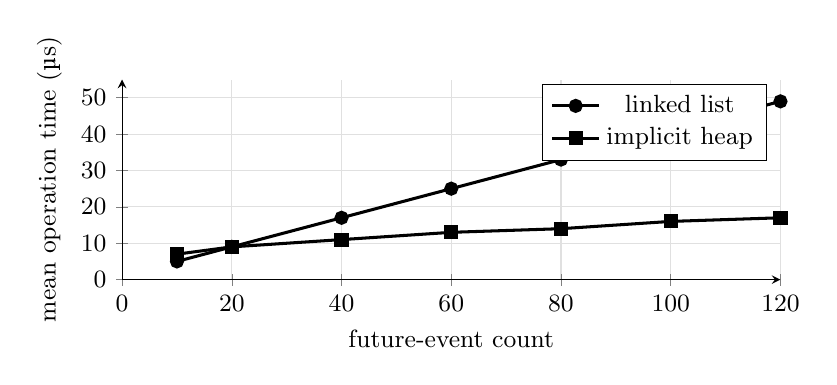
\begin{tikzpicture}
\begin{axis}[
  width=0.82\textwidth,height=0.34\textwidth,
  xmin=0,xmax=120,ymin=0,ymax=55,
  axis lines=left,
  xlabel={future-event count},
  ylabel={mean operation time (\textmu s)},
  xtick={0,20,40,60,80,100,120},
  ytick={0,10,20,30,40,50},
  ticklabel style={font=\small},
  label style={font=\small},
  legend style={font=\small,at={(0.98,0.98)},anchor=north east},
  grid=major,
  major grid style={draw=black!12}
]
\addplot[line width=1.1pt,mark=*] coordinates {
  (10,5) (20,9) (40,17) (60,25) (80,33) (100,41) (120,49)
};
\addlegendentry{linked list}
\addplot[line width=1.1pt,mark=square*] coordinates {
  (10,7) (20,9) (40,11) (60,13) (80,14) (100,16) (120,17)
};
\addlegendentry{implicit heap}
\end{axis}
\end{tikzpicture}
\caption{Mean Insert/Remove Times for Linked Lists and Implicit Heaps}
\label{fig:ext-smpl-event-performance}
\end{figure}

However, replacing the list is not always a net win:
\begin{itemize}
\item same-time FIFO ordering may need secondary keys,
\item event cancellation by event/token is naturally easy on lists,
\item if future-event count is small, list overhead is often acceptable.
\end{itemize}

The chapter recommends measuring typical list size and considering model
reformulation before changing core data structures.

\section{Storages}
\label{sec:ext-smpl-storages}

Storages model finite pools (memory, buffers, etc.) and are conceptually similar
to facilities but capacity-based.

Suggested API:
\begin{itemize}
\item \texttt{s = storage(name, n)},
\item \texttt{r = alloc(s, tkn, m)} (allocate $m$ units; queue if unavailable),
\item \texttt{dealloc(s, k)} (free $k$ units),
\item \texttt{m = avail(s)} (current free units).
\end{itemize}

\begin{figure}[ht]
\centering
\begin{tikzpicture}[>=Latex]
  \draw[line width=1pt] (0,0) rectangle (6.0,3.7);
  \draw[line width=0.8pt] (0,3.0) -- (6.0,3.0);
  \draw[line width=0.8pt] (0,2.3) -- (6.0,2.3);
  \draw[line width=0.8pt] (0,1.6) -- (6.0,1.6);
  \draw[line width=0.8pt] (3.2,0) -- (3.2,3.7);
  \node[font=\small] at (1.6,3.35) {name ptr};
  \node[font=\small] at (4.6,3.35) {queue head};
  \node[font=\small] at (1.6,2.65) {capacity};
  \node[font=\small] at (4.6,2.65) {available};
  \node[font=\small] at (1.6,1.95) {area stats};
  \node[font=\small] at (4.6,1.95) {time mark};
  \node[font=\small] at (1.6,1.25) {alloc count};
  \node[font=\small] at (4.6,1.25) {wait count};
  \node[font=\small] at (3.0,0.45) {storage descriptor};

  \draw[line width=1pt] (7.2,0.6) rectangle (12.4,3.1);
  \draw[line width=0.8pt] (7.2,2.4) -- (12.4,2.4);
  \draw[line width=0.8pt] (7.2,1.7) -- (12.4,1.7);
  \draw[line width=0.8pt] (9.8,0.6) -- (9.8,3.1);
  \node[font=\small] at (8.5,2.75) {token};
  \node[font=\small] at (11.1,2.75) {request $m$};
  \node[font=\small] at (8.5,2.05) {priority};
  \node[font=\small] at (11.1,2.05) {next/prev};
  \node[font=\small] at (9.8,1.15) {wait queue entry};
  \draw[->,line width=0.9pt] (6.1,2.8) -- (7.1,2.8);
\end{tikzpicture}
\caption{Storage Descriptor and Queue Structure}
\label{fig:ext-smpl-storage-structure}
\end{figure}

Key implementation points:
\begin{itemize}
\item descriptor can be built as a facility-structure variant,
\item queue-length and storage-utilization accumulators mirror facility logic,
\item deallocation may admit multiple waiting requests (discipline-dependent).
\end{itemize}

The text discusses FIFO, priority, and best-fit queue variants and the need to
extend reset/trace/report code paths accordingly.

\section{Tables}
\label{sec:ext-smpl-tables}

Tables collect empirical distributions of output variables (response time,
queueing delay, etc.).

\begin{figure}[ht]
\centering
\fbox{%
\begin{minipage}{0.9\textwidth}
\small\verbatimfont
TABLE: response\_time \quad range [0, 40], bins=10\\
count=5000 \quad mean=12.83 \quad stddev=4.27\\
------------------------------------------------------------\\
bin \quad from \quad to \quad freq \quad cum\_freq \quad prob\\
 1 \quad 0.0 \quad 4.0 \quad 112 \quad 112 \quad 0.022\\
 2 \quad 4.0 \quad 8.0 \quad 741 \quad 853 \quad 0.148\\
 3 \quad 8.0 \quad 12.0 \quad 1415 \quad 2268 \quad 0.283\\
 4 \quad 12.0 \quad 16.0 \quad 1328 \quad 3596 \quad 0.266\\
 5 \quad 16.0 \quad 20.0 \quad 804 \quad 4400 \quad 0.161\\
 6 \quad 20.0 \quad 24.0 \quad 363 \quad 4763 \quad 0.073\\
 7 \quad 24.0 \quad 28.0 \quad 148 \quad 4911 \quad 0.030\\
 8 \quad 28.0 \quad 32.0 \quad 66 \quad 4977 \quad 0.013\\
 9 \quad 32.0 \quad 36.0 \quad 18 \quad 4995 \quad 0.004\\
10 \quad 36.0 \quad 40.0 \quad 5 \quad 5000 \quad 0.001\\
\end{minipage}}
\caption{\texttt{smpl} Table Report}
\label{fig:ext-smpl-table-report}
\end{figure}

Definition and entry interface:
\begin{itemize}
\item \texttt{t = table(from, to, n, opt, name)},
\item \texttt{enter(v, t)}.
\end{itemize}

Descriptor fields include lower bound, interval width, option flags, number of
cells, entry count, sums for mean/variance, and underflow/overflow counters.

\begin{figure}[ht]
\centering
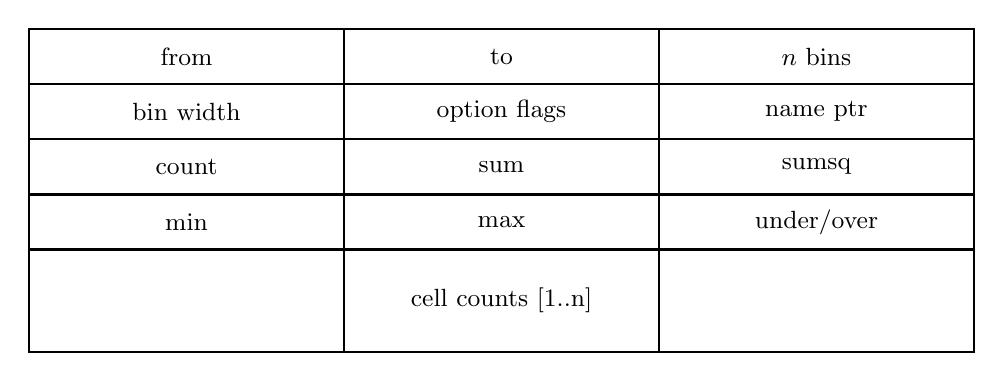
\begin{tikzpicture}
  \draw[line width=1pt] (0,0) rectangle (12,4.1);
  \draw[line width=0.8pt] (0,3.4) -- (12,3.4);
  \draw[line width=0.8pt] (0,2.7) -- (12,2.7);
  \draw[line width=0.8pt] (0,2.0) -- (12,2.0);
  \draw[line width=0.8pt] (0,1.3) -- (12,1.3);
  \draw[line width=0.8pt] (4.0,0) -- (4.0,4.1);
  \draw[line width=0.8pt] (8.0,0) -- (8.0,4.1);
  \node[font=\small] at (2.0,3.75) {from};
  \node[font=\small] at (6.0,3.75) {to};
  \node[font=\small] at (10.0,3.75) {$n$ bins};
  \node[font=\small] at (2.0,3.05) {bin width};
  \node[font=\small] at (6.0,3.05) {option flags};
  \node[font=\small] at (10.0,3.05) {name ptr};
  \node[font=\small] at (2.0,2.35) {count};
  \node[font=\small] at (6.0,2.35) {sum};
  \node[font=\small] at (10.0,2.35) {sumsq};
  \node[font=\small] at (2.0,1.65) {min};
  \node[font=\small] at (6.0,1.65) {max};
  \node[font=\small] at (10.0,1.65) {under/over};
  \node[font=\small] at (6.0,0.65) {cell counts [1..n]};
\end{tikzpicture}
\caption{Table Descriptor}
\label{fig:ext-smpl-table-descriptor}
\end{figure}

On each \texttt{enter()}, the code updates:
\begin{itemize}
\item count, sum, sum-of-squares,
\item min/max,
\item underflow/overflow or selected cell count.
\end{itemize}

The chapter notes that fixed ranges can be inconvenient when location/shape are
unknown; adaptive histogram methods are possible alternatives.

\section{Distributions}
\label{sec:ext-smpl-distributions}

Distribution definition is separated from sampling:
\begin{itemize}
\item \texttt{d = distr(type, p1, p2)},
\item \texttt{v = sample(d)}.
\end{itemize}

This decoupling improves parameterized model setup, debugging, and supports
variance-reduction patterns.

\begin{figure}[ht]
\centering
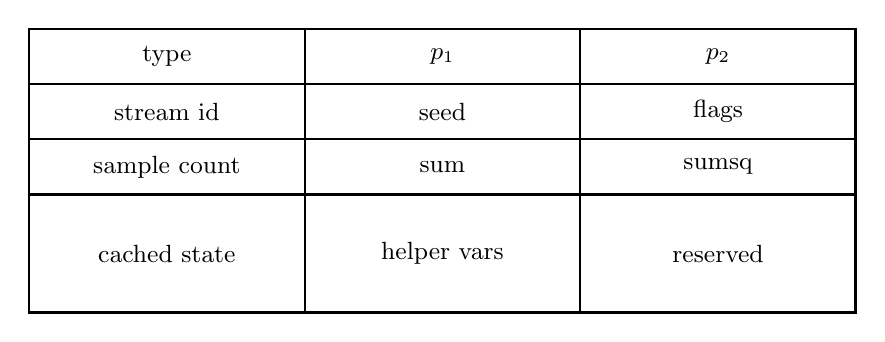
\begin{tikzpicture}
  \draw[line width=1pt] (0,0) rectangle (10.5,3.6);
  \draw[line width=0.8pt] (0,2.9) -- (10.5,2.9);
  \draw[line width=0.8pt] (0,2.2) -- (10.5,2.2);
  \draw[line width=0.8pt] (0,1.5) -- (10.5,1.5);
  \draw[line width=0.8pt] (3.5,0) -- (3.5,3.6);
  \draw[line width=0.8pt] (7.0,0) -- (7.0,3.6);
  \node[font=\small] at (1.75,3.25) {type};
  \node[font=\small] at (5.25,3.25) {$p_1$};
  \node[font=\small] at (8.75,3.25) {$p_2$};
  \node[font=\small] at (1.75,2.55) {stream id};
  \node[font=\small] at (5.25,2.55) {seed};
  \node[font=\small] at (8.75,2.55) {flags};
  \node[font=\small] at (1.75,1.85) {sample count};
  \node[font=\small] at (5.25,1.85) {sum};
  \node[font=\small] at (8.75,1.85) {sumsq};
  \node[font=\small] at (1.75,0.75) {cached state};
  \node[font=\small] at (5.25,0.75) {helper vars};
  \node[font=\small] at (8.75,0.75) {reserved};
\end{tikzpicture}
\caption{Distribution Descriptor}
\label{fig:ext-smpl-distribution-descriptor}
\end{figure}

Each distribution can maintain its own stream seed. That enables:
\begin{itemize}
\item common random numbers across alternatives,
\item antithetic variants (via complemented seed handling).
\end{itemize}

An example type set is proposed:
\texttt{constant}, \texttt{uniform}, \texttt{normal}, \texttt{expntl}
(with Erlang/expntl/hyperexponential selection from mean/stddev relation).

\section{A Run-Time Interface}
\label{sec:ext-smpl-runtime}

The chapter emphasizes that a run-time interface is usually the highest-leverage
extension. In SMPL/PC this role is handled by \texttt{mtr}.

\begin{figure}[ht]
\centering
\begin{tikzpicture}[>=Latex,node distance=1.0cm and 1.5cm]
  \node[draw,rounded corners,minimum width=3.6cm,minimum height=0.9cm] (start) {\texttt{smpl()} startup};
  \node[draw,minimum width=3.8cm,minimum height=0.9cm,below=of start] (i1) {\texttt{init\_mtr()} phase 1};
  \node[draw,minimum width=4.4cm,minimum height=0.9cm,below=of i1] (model) {model defines facilities/parameters};
  \node[draw,minimum width=3.8cm,minimum height=0.9cm,below=of model] (i2) {\texttt{init\_mtr()} phase 2};
  \node[draw,minimum width=3.4cm,minimum height=0.9cm,below=of i2] (loop) {\texttt{cause()} event loop};
  \node[draw,diamond,aspect=1.7,below=of loop] (check) {pause/break/error?};
  \node[draw,minimum width=3.2cm,minimum height=0.9cm,left=2.8cm of check] (mtr) {\texttt{mtr()} command handler};
  \node[draw,minimum width=3.2cm,minimum height=0.9cm,below=of check] (run) {continue execution};

  \draw[->,line width=0.9pt] (start) -- (i1);
  \draw[->,line width=0.9pt] (i1) -- (model);
  \draw[->,line width=0.9pt] (model) -- (i2);
  \draw[->,line width=0.9pt] (i2) -- (loop);
  \draw[->,line width=0.9pt] (loop) -- (check);
  \draw[->,line width=0.9pt] (check) -- node[above,font=\small] {yes} (mtr);
  \draw[->,line width=0.9pt] (mtr) |- (loop);
  \draw[->,line width=0.9pt] (check) -- node[right,font=\small] {no} (run);
  \draw[->,line width=0.9pt] (run) |- (loop);
\end{tikzpicture}
\caption{\texttt{mtr} Initialization and Control Functions}
\label{fig:ext-smpl-mtr-flow}
\end{figure}

Integration points:
\begin{itemize}
\item \texttt{init\_mtr()} called twice from \texttt{smpl} init path
  (before and after facility definition),
\item \texttt{mtr()} called during execution (typically from \texttt{cause()}),
\item optional pause/error hooks.
\end{itemize}

Suggested first features:
\begin{itemize}
\item trace control,
\item report display/reset,
\item parameter display and editing.
\end{itemize}

Parameter support (\texttt{parms} module) uses calls like:
\begin{itemize}
\item \texttt{pdef(num, ptr, name)},
\item lookup helpers by number/pointer.
\end{itemize}

These parameters are then reused by breakpoints, table setup, analysis displays,
and run-time experimentation.

\section{In Conclusion}
\label{sec:ext-smpl-conclusion}

The chapter closes with two practical recommendations:
\begin{enumerate}
\item build a usable run-time interface early, then grow extensions around it;
\item use \texttt{smpl} for small-to-medium models and as a compact simulation
  kernel for specialized tooling.
\end{enumerate}

For large, highly detailed models, process-oriented languages are generally more
natural. Regardless of language, begin with small/high-leverage models early in
design and scale detail incrementally.

\appendix
% OCR draft from PDF pages 280-298 (Appendix source listings).
\chapter{Appendix}
\label{chap:appendix-source}

The following pages in the original book provide C source listings for four
files:
\begin{itemize}
\item \texttt{smpl.c}: the SMPL simulation subsystem (excluding random variates),
\item \texttt{rand.c}: random variate generation functions,
\item \texttt{smpl.h}: external declarations and user-level directives,
\item \texttt{stat.c}: normal and $t$-distribution quantile support.
\end{itemize}

An executable model is formed by compiling \texttt{smpl.c} and \texttt{rand.c}
(or packaging them in a library), and compiling/linking the simulation model
source that includes \texttt{smpl.h}.

\section{Listing Overview}
\label{sec:appendix-listing-overview}

\begin{itemize}
\item \textbf{\texttt{smpl.c}} (pp.~281--293 in the scan): initialization, element
  pool management, event scheduling, queue/list processing, facility
  operations, tracing, and report output.
\item \textbf{\texttt{rand.c}} (pp.~294--297): stream/seed handling and variate
  generators (\texttt{ranf}, \texttt{random}, \texttt{expntl}, \texttt{erlang},
  \texttt{hyperx}, \texttt{normal}).
\item \textbf{\texttt{stat.c}} (p.~298 onward): quantile routines used by analysis
  modules.
\end{itemize}

\section{Implementation Notes}
\label{sec:appendix-notes}

The scanned appendix is code-heavy and OCR introduces substantial formatting
noise (spacing, punctuation, and token corruption in identifiers/operators).
For this draft, code is represented as structural overview text. A later pass can
replace this with validated verbatim listings (or with cleaned source imported
from trusted machine-readable files).


\backmatter
% OCR draft from PDF pages 299-306.
\chapter{References}
\label{chap:references}

The source scan includes an extensive bibliography (pp.~299--306), covering
simulation methodology, queueing analysis, random variate generation,
validation, and computer/network performance modeling.

Key recurring authors/themes in this bibliography include:
\begin{itemize}
\item simulation output analysis and confidence intervals,
\item queueing theory and operational analysis,
\item random number generation and variance-reduction methods,
\item local-area network and Ethernet performance studies,
\item multiprocessor and cache/coherency performance models.
\end{itemize}

Representative entries visible in OCR include works by Allen, Banks, Bratley,
Fishman, Kobayashi, Law and Kelton, Lavenberg, MacNair and Sauer, Schrage,
and Sargent, among others.

% NOTE: Full per-entry transcription is pending a dedicated bibliography pass.

% OCR draft from PDF pages 307-314.
\chapter{Indexes}
\label{chap:indexes}

\section*{Author Index}

The scan includes a detailed author index (pp.~307--308). It maps cited authors
to discussion pages across topics such as queueing analysis, simulation
validation, random variate generation, and performance modeling.

\section*{Subject Index}

The subject index (pp.~309--314) covers operational terms and model concepts,
including:
\begin{itemize}
\item confidence interval estimation (fixed-sample and batch-means),
\item verification and validation workflows,
\item queueing/facility operations in \texttt{smpl},
\item event scheduling and trace/report functions,
\item token ring, Ethernet, and multiprocessor model topics.
\end{itemize}

% NOTE: Full index-entry transcription is pending a dedicated indexing pass.

\end{document}
